% Options for packages loaded elsewhere
% Options for packages loaded elsewhere
\PassOptionsToPackage{unicode}{hyperref}
\PassOptionsToPackage{hyphens}{url}
\PassOptionsToPackage{dvipsnames,svgnames,x11names}{xcolor}
%
\documentclass[
  spanish,
  a4paper,
]{scrreprt}
\usepackage{xcolor}
\usepackage{amsmath,amssymb}
\setcounter{secnumdepth}{5}
\usepackage{iftex}
\ifPDFTeX
  \usepackage[T1]{fontenc}
  \usepackage[utf8]{inputenc}
  \usepackage{textcomp} % provide euro and other symbols
\else % if luatex or xetex
  \usepackage{unicode-math} % this also loads fontspec
  \defaultfontfeatures{Scale=MatchLowercase}
  \defaultfontfeatures[\rmfamily]{Ligatures=TeX,Scale=1}
\fi
\usepackage{lmodern}
\ifPDFTeX\else
  % xetex/luatex font selection
\fi
% Use upquote if available, for straight quotes in verbatim environments
\IfFileExists{upquote.sty}{\usepackage{upquote}}{}
\IfFileExists{microtype.sty}{% use microtype if available
  \usepackage[]{microtype}
  \UseMicrotypeSet[protrusion]{basicmath} % disable protrusion for tt fonts
}{}
% Make \paragraph and \subparagraph free-standing
\makeatletter
\ifx\paragraph\undefined\else
  \let\oldparagraph\paragraph
  \renewcommand{\paragraph}{
    \@ifstar
      \xxxParagraphStar
      \xxxParagraphNoStar
  }
  \newcommand{\xxxParagraphStar}[1]{\oldparagraph*{#1}\mbox{}}
  \newcommand{\xxxParagraphNoStar}[1]{\oldparagraph{#1}\mbox{}}
\fi
\ifx\subparagraph\undefined\else
  \let\oldsubparagraph\subparagraph
  \renewcommand{\subparagraph}{
    \@ifstar
      \xxxSubParagraphStar
      \xxxSubParagraphNoStar
  }
  \newcommand{\xxxSubParagraphStar}[1]{\oldsubparagraph*{#1}\mbox{}}
  \newcommand{\xxxSubParagraphNoStar}[1]{\oldsubparagraph{#1}\mbox{}}
\fi
\makeatother


\usepackage{longtable,booktabs,array}
\newcounter{none} % for unnumbered tables
\usepackage{calc} % for calculating minipage widths
% Correct order of tables after \paragraph or \subparagraph
\usepackage{etoolbox}
\makeatletter
\patchcmd\longtable{\par}{\if@noskipsec\mbox{}\fi\par}{}{}
\makeatother
% Allow footnotes in longtable head/foot
\IfFileExists{footnotehyper.sty}{\usepackage{footnotehyper}}{\usepackage{footnote}}
\makesavenoteenv{longtable}
\usepackage{graphicx}
\makeatletter
\newsavebox\pandoc@box
\newcommand*\pandocbounded[1]{% scales image to fit in text height/width
  \sbox\pandoc@box{#1}%
  \Gscale@div\@tempa{\textheight}{\dimexpr\ht\pandoc@box+\dp\pandoc@box\relax}%
  \Gscale@div\@tempb{\linewidth}{\wd\pandoc@box}%
  \ifdim\@tempb\p@<\@tempa\p@\let\@tempa\@tempb\fi% select the smaller of both
  \ifdim\@tempa\p@<\p@\scalebox{\@tempa}{\usebox\pandoc@box}%
  \else\usebox{\pandoc@box}%
  \fi%
}
% Set default figure placement to htbp
\def\fps@figure{htbp}
\makeatother


% definitions for citeproc citations
\NewDocumentCommand\citeproctext{}{}
\NewDocumentCommand\citeproc{mm}{%
  \begingroup\def\citeproctext{#2}\cite{#1}\endgroup}
\makeatletter
 % allow citations to break across lines
 \let\@cite@ofmt\@firstofone
 % avoid brackets around text for \cite:
 \def\@biblabel#1{}
 \def\@cite#1#2{{#1\if@tempswa , #2\fi}}
\makeatother
\newlength{\cslhangindent}
\setlength{\cslhangindent}{1.5em}
\newlength{\csllabelwidth}
\setlength{\csllabelwidth}{3em}
\newenvironment{CSLReferences}[2] % #1 hanging-indent, #2 entry-spacing
 {\begin{list}{}{%
  \setlength{\itemindent}{0pt}
  \setlength{\leftmargin}{0pt}
  \setlength{\parsep}{0pt}
  % turn on hanging indent if param 1 is 1
  \ifodd #1
   \setlength{\leftmargin}{\cslhangindent}
   \setlength{\itemindent}{-1\cslhangindent}
  \fi
  % set entry spacing
  \setlength{\itemsep}{#2\baselineskip}}}
 {\end{list}}
\usepackage{calc}
\newcommand{\CSLBlock}[1]{\hfill\break\parbox[t]{\linewidth}{\strut\ignorespaces#1\strut}}
\newcommand{\CSLLeftMargin}[1]{\parbox[t]{\csllabelwidth}{\strut#1\strut}}
\newcommand{\CSLRightInline}[1]{\parbox[t]{\linewidth - \csllabelwidth}{\strut#1\strut}}
\newcommand{\CSLIndent}[1]{\hspace{\cslhangindent}#1}

\ifLuaTeX
\usepackage[bidi=basic,shorthands=off]{babel}
\else
\usepackage[bidi=default,shorthands=off]{babel}
\fi
\ifLuaTeX
  \usepackage{selnolig} % disable illegal ligatures
\fi


\setlength{\emergencystretch}{3em} % prevent overfull lines

\providecommand{\tightlist}{%
  \setlength{\itemsep}{0pt}\setlength{\parskip}{0pt}}



 


\makeatletter
  \renewenvironment{quote}
     {\list{}{\listparindent 1.5em%
              \itemindent \listparindent
              \rightmargin \leftmargin
              \parsep \z@ \@plus \p@}%
            \item\noindent\relax}
      {\endlist}
  \makeatother
\usepackage{booktabs}
\usepackage{caption}
\usepackage{longtable}
\usepackage{colortbl}
\usepackage{array}
\usepackage{anyfontsize}
\usepackage{multirow}
\makeatletter
\@ifpackageloaded{tcolorbox}{}{\usepackage[skins,breakable]{tcolorbox}}
\@ifpackageloaded{fontawesome5}{}{\usepackage{fontawesome5}}
\definecolor{quarto-callout-color}{HTML}{909090}
\definecolor{quarto-callout-note-color}{HTML}{0758E5}
\definecolor{quarto-callout-important-color}{HTML}{CC1914}
\definecolor{quarto-callout-warning-color}{HTML}{EB9113}
\definecolor{quarto-callout-tip-color}{HTML}{00A047}
\definecolor{quarto-callout-caution-color}{HTML}{FC5300}
\definecolor{quarto-callout-color-frame}{HTML}{acacac}
\definecolor{quarto-callout-note-color-frame}{HTML}{4582ec}
\definecolor{quarto-callout-important-color-frame}{HTML}{d9534f}
\definecolor{quarto-callout-warning-color-frame}{HTML}{f0ad4e}
\definecolor{quarto-callout-tip-color-frame}{HTML}{02b875}
\definecolor{quarto-callout-caution-color-frame}{HTML}{fd7e14}
\makeatother
\makeatletter
\@ifpackageloaded{bookmark}{}{\usepackage{bookmark}}
\makeatother
\makeatletter
\@ifpackageloaded{caption}{}{\usepackage{caption}}
\AtBeginDocument{%
\ifdefined\contentsname
  \renewcommand*\contentsname{Tabla de contenidos}
\else
  \newcommand\contentsname{Tabla de contenidos}
\fi
\ifdefined\listfigurename
  \renewcommand*\listfigurename{Listado de Figuras}
\else
  \newcommand\listfigurename{Listado de Figuras}
\fi
\ifdefined\listtablename
  \renewcommand*\listtablename{Listado de Tablas}
\else
  \newcommand\listtablename{Listado de Tablas}
\fi
\ifdefined\figurename
  \renewcommand*\figurename{Figura}
\else
  \newcommand\figurename{Figura}
\fi
\ifdefined\tablename
  \renewcommand*\tablename{Tabla}
\else
  \newcommand\tablename{Tabla}
\fi
}
\@ifpackageloaded{float}{}{\usepackage{float}}
\floatstyle{ruled}
\@ifundefined{c@chapter}{\newfloat{codelisting}{h}{lop}}{\newfloat{codelisting}{h}{lop}[chapter]}
\floatname{codelisting}{Listado}
\newcommand*\listoflistings{\listof{codelisting}{Listado de Listados}}
\makeatother
\makeatletter
\makeatother
\makeatletter
\@ifpackageloaded{caption}{}{\usepackage{caption}}
\@ifpackageloaded{subcaption}{}{\usepackage{subcaption}}
\makeatother

\usepackage{bookmark}
\IfFileExists{xurl.sty}{\usepackage{xurl}}{} % add URL line breaks if available
\urlstyle{same}
\hypersetup{
  pdftitle={Taller Muestreo},
  pdfauthor={Recursos Didácticos y Tecnológicos para la Enseñanza},
  pdflang={es},
  colorlinks=true,
  linkcolor={blue},
  filecolor={Maroon},
  citecolor={Blue},
  urlcolor={Blue},
  pdfcreator={LaTeX via pandoc}}


\title{Taller Muestreo}
\author{Recursos Didácticos y Tecnológicos para la Enseñanza}
\date{13 de febrero de 2026}
\begin{document}
\cleardoublepage
\thispagestyle{empty}
{\centering
\hbox{}\vskip 0cm plus 1fill
{\Huge\bfseries Taller Muestreo \par}
\vspace{3ex}
{\bfseries\large Versión 1.0.1 \par}
\vspace{12ex}
{\Large\bfseries Recursos Didácticos y Tecnológicos para la
Enseñanza \par}
\vspace{3ex}
%
%
{\bfseries\large  \par}
\vspace{12ex}
%
%
{\bfseries\large Subsecretaria de Planeamiento Educativo - PBA \par}
\vspace{12ex}
%
%
{\bfseries\large  \par}
\vspace{12ex}
%
%
{\bfseries\large  \par}
\vspace{12ex}
%
\vspace{12ex}
{\bfseries\large 13 de febrero de 2026 \par}
\vspace{12ex}
{\small Versión PDF. Consultar versión online para una experiencia más interactiva en https://planificacion-muestreo.netlify.app/ \par}
}

\let\mainmatterreal\mainmatter
\let\mainmatter\relax
\renewcommand*\contentsname{Tabla de contenidos}
\hypersetup{linkcolor=}
\setcounter{tocdepth}{2}
\renewcommand*\listfigurename{List of figures}
\renewcommand*\listtablename{List of tables}
\noindent 

\bookmarksetup{startatroot}

\chapter{Introducción}\label{sec-introduccion}

En este curso/taller vamos a ir interactuando entre algo de teoría, algo
de datos y algo de código. Generalmente, vamos a trabajar con un solo
insumo empírico que es una base de datos de establecimientos educativos
de nivel primario de gestión estatal de la provincia de Buenos Aires.
Con este insumo en una primera instancia nos vamos a focalizar en una
serie de \emph{diseños} clásicos de muestreo y en la construcción de
ponderadores. En una segunda instancia vamos a ver diseños que implican:

a) Alguna combinación en más de un paso de estos diseños clásicos
(muestras complejas) o

b) diseños de un solo paso cuyos supuestos o modo de proceder son algo
diferentes al de los clásicos (p.e. diseños balanceados y bien
distribuidos).

Finalmente, se verán algunas estrategias de calibración que, en
principio, al ser instancias post-diseños, pueden ser
aplicadas/combinadas con cualquiera de los anteriores diseños.

El código con que vamos a procesar los datos a lo largo del taller va a
ser en lenguaje R. R es un lenguaje de programación que parece una
opción razonable tanto para el diseño de la muestra como su posterior
calibración y análisis de los datos. Si bien diseños de métodos de
muestreo relativamente simples son posibles de realizarse en varios
otros lenguajes la situación se complica un poco a medida que se quieren
utilizar, y luego analizar, diseños más complejos. En esta última
situación, ya no es posible conseguir librerías especializadas en muchos
lenguajes aparte de R, Python, Julia y SAS.

Dentro del ecosistema de R, ejemplos de librerías para analizar datos
producidos con diseños muestrales pueden considerarse
\href{https://r-survey.r-forge.r-project.org/survey/}{survey},
\href{https://bschneidr.github.io/svrep/}{svrep} y su correspondiente
versión tidy \href{http://gdfe.co/srvyr/}{srvyr}. Estas librerías
generalmente agregan meta-información al dataframe original que hace
referencia al modo o diseño en que fue realizada la muestra. Esta
información luego es utilizada para realizar estimaciones puntuales con
sus respectivos errores estandard, intervalos de confianza o
coeficientes de variación. La librería survey es una librería madura
mantenida principalmente por
\href{https://en.wikipedia.org/wiki/Thomas_Lumley_(statistician)}{Thomas
Lumley} (un personaje conocido dentro de la comunidad estadística en
general y en la en R en particular). La librería srvyr puede
considerarse como su sucesora más moderna, aunque como lo destacan sus
propios autores, se trata de una librería más amigable para el usuario
en donde la mayoría del trabajo sucio lo sigue haciendo por detrás la
librería survey. Algo similar resulta entre la relación entre survey y
svrep ya que esta última se puede considerar una extensión de la primera
para el cálculo de ponderadores replicados (\emph{replicate weights}).
Algo importante a destacar es la compatibilidad entre las 3 librerías y
que, a pesar de la diferencia generacional (Lumley es el mayor) existe
una relación afectuosa entre los diferentes autores. En efecto,
\href{https://github.com/bschneidr}{Ben Schneider}, el creador de la
librería svrep, es un asiduo contribuidor de los 3 paquetes antes
nombrados.\footnote{Existen más librerías que pueden considerarse como
  extensiones de survey.
  \href{https://cran.r-project.org/web/packages/robsurvey/index.html}{robsurvey},
  para la realización de estimaciones robustas, es otro ejemplo.}

Ejemplos de librerías que sirven para el diseño de las muestras y su
posterior ajuste son
\href{https://cran.r-project.org/web/packages/sampling/index.html}{sampling},
\href{https://envisim.se/balancedsampling}{balanced sampling} y
\href{https://cran.r-project.org/web/packages/Spbsampling/index.html}{spbsampling}.
Al igual que con las librerías anteriores, aquí también existe relación
entre los diferentes autores. La librería sampling es una librería
madura creada bajo la tutela de Yver Tillé, que es otro personaje
bastante conocido tanto en el mundo de la estadística académica como
dentro de los organismos oficiales de estadística de diferentes países.
La librería balanced sampling hace mucho de las funciones que la
librería sampling, pero es más moderna (corre en C\textsuperscript{++})
y es mantenida por
\href{https://scholar.google.com/citations?user=JkMAOUEAAAAJ&hl=sv}{Anton
Grafstrom} que ha escrito con Tillé. Por otro lado, la librería
spbsampling se especializa en muestreos espaciales (balanced sampling
también tiene funciones para eso), se ejecuta en C\textsuperscript{++} y
es mantenida por
\href{https://scholar.google.com/citations?user=h_Rnt4kAAAAJ&hl=it}{Roberto
Benedetti}. Tanto Benedetti como Grafstrom se reconocen entre ellos y
algo interesante es que si, bien ambos han trabajado con institutos
oficiales de estadística, ambos se especializan en organismos de
agricultura. De ahí que ambos muestren interés en la dimensión espacial
de los diseños muestrales porque esta es útil a la hora de, por ejemplo,
diseñar una buena muestra de la vegetación de un bosque.\footnote{Para
  aquel que le interesa agregar explícitamente la dimensión espacial en
  los diseños muestrales puede consultar la obra de Dick Brus
  ``\href{https://dickbrus.github.io/SpatialSamplingwithR/}{Spatial
  sampling with R}''. Brus, un geólogo ahora ya retirado, es una
  eminencia mundial en la temática de los muestreos de suelo (\emph{soil
  sampling}) y más en general, de los muestreos espaciales.}

Por último, para el cálculo de los tamaños muestrales con diferentes
diseños (y otras yerbas) puede consultarse la librería
\href{https://cran.r-project.org/web/packages/PracTools/index.html}{PracTools}.
No se trata de una libraría muy sofisticada como algunas de las
anteriores pero se trata de una librería útil y relativamente bien
documentada. Un dato no menor es que uno de sus autores es
\href{https://scholar.google.com/citations?user=6Q5RKeAAAAAJ&hl=en}{Richard
Valliant} que, a su turno, es uno de los mayores exponentes de un
enfoque importante dentro del mundo del muestreo como es el
``\emph{Model Assisted Sampling}''. \footnote{Otras librerías que
  existen dentro del ecosistema de R pero que no veremos aquí son
  \href{https://barcaroli.github.io/SamplingStrata/}{SamplingStrata} y
  \href{https://csblatvia.github.io/surveyplanning/}{surveyplanning}.}

\section{Librerías utilizadas}\label{libreruxedas-utilizadas}

Abajo hay un código para instalar y cargar las librerías que vamos a
utilizar. El código se encarga de cargar las librerías y de instalar las
mismas en el caso de que no se encuentren previamente instaladas.

\bookmarksetup{startatroot}

\chapter{Cuándo y por qué hacer
muestras}\label{cuuxe1ndo-y-por-quuxe9-hacer-muestras}

Una muestra es una parte de un todo. En los muestreos que aspiran a ser
(en algún grado) representativos lo que se intenta lograr es que esa
parte que se seleccione no sea muy diferente al todo o, como decían los
romanos, que sea legítimo tomar una parte como el todo (\emph{pars pro
toto}). En este sentido, lo que vamos a hablar aquí sobre muestreo tiene
mayor pertinencia cuando en la investigación se intenta maximizar la
\textbf{representatividad}, pero por alguna razón no es posible o
conveniente la realización de un censo de todas las partes que conforman
ese todo. Por otro lado, diseñar muestras también puede ser importante
cuando se necesitan construir grupos de tratamiento y control en diseños
experimentales, especialmente en los diseños experimentales aleatorios
(Kish 1987). En efecto, la vinculación entre la bibliografía de los
diseños muestrales y los diseños experimentales suele ser útil si se
aspira a entender las razones (y no solo saber ejecutarlas en la
práctica) de algunas recomendaciones metodológicas, ya que muchos de los
conceptos más abstractos son compartidos por ambas {[}Hedlin
(2015){]}(Fienberg y Tanur 1988).

\begin{tcolorbox}[enhanced jigsaw, leftrule=.75mm, title=\textcolor{quarto-callout-note-color}{\faInfo}\hspace{0.5em}{Nota}, colframe=quarto-callout-note-color-frame, coltitle=black, breakable, opacityback=0, bottomtitle=1mm, opacitybacktitle=0.6, rightrule=.15mm, titlerule=0mm, toprule=.15mm, colbacktitle=quarto-callout-note-color!10!white, left=2mm, toptitle=1mm, bottomrule=.15mm, arc=.35mm, colback=white]

Las muestras que aspiran a ser representativas intentan captar la
heterogeneidad de una determinada población para poder hablar
legítimamente del todo a través de solo una parte.

\end{tcolorbox}

En algunas situaciones, más usuales en las ciencias naturales, la
representatividad a veces se logra sin un mayor esfuerzo por parte del
investigador por lo que no suele ser explícitamente un objetivo de la
investigación sino un supuesto más o menos implícito a lo largo de ella.
En otras palabras, la hipótesis de la homogeneidad forma parte del
modelo mediante el cual se intenta aprendeder de la realidad. Entender
la razón de esto último puede ayudar a hacer más transparente alguna
especificidad de las ciencias sociales en este punto. En efecto, muchos
investigadores consideran que en los niveles más bajos de la realidad
(p.e. niveles estudiados por la física y la química) existe una mayor
homogeneidad de los referentes básicos que estudian esas disciplinas. En
cambio, en los niveles más superiores (p.e. niveles estudiados por
ejemplo por la psicología y las ciencias sociales) la variabilidad
inherentes de los referentes estudiados hace que sea necesario prestar
especial atención al problema de la representatividad, En este sentido,
el investigador suele realizar acciones específicas para poder captar la
heterogeneidad que surge a nivel poblacional debido a la variabilidad
individual de los referentes estudiados y, en ese camino, suele venir en
ayuda el diseño muestral.

De manera derivada, lo anterior es una de las razones por lo cual el
método experimental ha sido bastante exitoso en la historia de las
ciencias naturales, ya que con unos pocos experimentos sus resultados se
pueden inferir a su respectiva \textbf{población} empírica actual. No
solo eso. Muchas veces también se puede inferir a lo que a veces se
denomina su \textbf{universo} que estaría compuesto no solo por la
población actual sino también por la clase de esas poblaciones pasadas y
futuras. Este tipo de problemáticas son conocidas por diferentes
disciplinas. Desde la epistemología a veces se los relaciona con el
problema de los universales (Klima 2022) y desde la metodología se lo
relaciona con el problema de la \textbf{validez externa} de las
investigaciones (Campbell y Stanley 1963).\\
\strut \\
A modo de ejemplo, un físico que investiga el impacto del calor en el
átomo de carbono puede tener una razonable confianza que el átomo de
carbono que está hoy estudiando no solo es muy similar a los otros
átomos de carbono actuales en la Tierra (población) sino que también es
similar a los pasados y los futuros átomos de carbono (universo).
También puede tener confianza que los átomos de carbono encontrados en
la Tierra son similares a los existentes en el resto del universo. En el
otro extremo, este tipo de suposiciones en general son difíciles de
mantener en el nivel social.

Estas diferencias en cuanto a la validez externa no son tan marcadas
cuanto se analiza la dimensión de la \textbf{validez interna} de las
investigaciones. En la jerga de la bibliografía de los diseños de
investigación se suele afirmar que en todas las investigaciones que se
quiera realizar inferencias causales, independientemente si se trata de
investigaciones físicas o sociales, el investigador se debe asegurar, en
la fase de diseño de la investigación, de controlar o aleatorizar el
conjunto de factores extraños que le sugiera/n la o las teorías
utilizadas. Esto es lo que precisamente le asegurará que aquellos
factores extraños no sigan existiendo como factores perturbadores que
puedan invalidar las inferencias internas o locales en el momento de las
conclusiones (Kish 1987). En el último tiempo la visión anterior se ha
expandido aún más permitiendo mayor seguridad en diseños observacionales
en situaciones en donde no es posible un diseño experimental aleatorio
lo que es sumamente importante en el dominio de las ciencias sociales
(Pearl 2018; Morgan y Winship 2015).

Dada la introducción anterior, ahora estamos en condiciones de expresar
lo mismo pero en términos más simples:

\begin{tcolorbox}[enhanced jigsaw, leftrule=.75mm, title=\textcolor{quarto-callout-note-color}{\faInfo}\hspace{0.5em}{Nota}, colframe=quarto-callout-note-color-frame, coltitle=black, breakable, opacityback=0, bottomtitle=1mm, opacitybacktitle=0.6, rightrule=.15mm, titlerule=0mm, toprule=.15mm, colbacktitle=quarto-callout-note-color!10!white, left=2mm, toptitle=1mm, bottomrule=.15mm, arc=.35mm, colback=white]

Donde no hay heterogeneidad con seguridad no hay problemas de
representatividad. Si hay heterogeneidad, y el investigador no realiza
acciones en su diseño para incluir esa heterogeneidad en su
investigación, la misma sufrirá de un problema de representatividad que
derivará en un problema de \textbf{validez externa}.

\end{tcolorbox}

\section{¿Muestras de qué?}\label{muestras-de-quuxe9}

\hfill\break
Un primer paso importante cuando uno se preocupa por la
representatividad es entender sobre qué población de referentes y de
unidades de observación/experimentación uno va a querer predicar sus
inferencias. Para eso hay que analizar:~\\
\strut \\
a) La clase de referencia de los conceptos utilizados que nos dirá
el/los tipo/s de referente/s a investigar (individuos, organizaciones,
etc.). Esto a veces se suele denominar \textbf{universo} o dominio de la
teoría (Bunge 1974).

b) Los objetivos de la investigación que nos indicaran, entre otras
cuestiones, el alcance (usualmente especificando tiempo y espacio) de
los referentes anteriores junto con otras características pertinentes de
cada unidad de observación/experimentación. Usualmente los objetivos
remiten a una población empírica que podrá grande o pequeña, homogénea o
heterogénea, dispersa o aglomerada, etc.~\\
\strut \\
Dentro del muestreo al conjunto formado por todos los objetos reales que
cumplan las condiciones de los puntos ``a'' y ``b'' se lo denomina
\textbf{población}\footnote{Expresado en términos de propiedades
  generales y específicas podría afirmarse que las~\textbf{propiedades
  generales}, como su nombre lo indica, sirven para construir
  \textbf{géneros} y todos los objetos reales que pertenecen a ese
  género tienen el mismo valor en todas sus propiedades generales.
  Ejemplo: Todo objeto real que se clasifique como ``persona'' deberá
  cumplir una serie de propiedades generales que hacen a la esencia de
  ``persona'' y se incluyen en su definición. Ser estudiante o residir
  en la provincia de Buenos Aires no pertenece a un valor de una
  propiedad general de las personas. En cambio, mamífero descendiente
  del mono, sí. Las propiedades generales son necesarias para
  identificar la clase de referencia, pero no suficientes para construir
  la población sobre la cual se realizará la muestra.~

  Las~\textbf{propiedades específicas,} también como su nombre lo
  sugiere\textbf{,}~sirven para construir \textbf{especies de los
  géneros} en función de los diferentes valores en las propiedades
  específicas. Tiempo y espacio son típicas propiedades específicas que
  ayudan recortar al universo anterior delimitando una población
  empírica. Luego pueden existir otras propiedades específicas (como las
  anteriores de ser estudiante o vivir en Buenos Aires) que sirven para
  seguir delimitando aún más nuestra población.}.~En nuestra vida
cotidiana, aunque sea solo por vivir en un tiempo y espacio determinado
(y aun si somos investigadores de profesión) usualmente solo tenemos
posibilidad de acceso empírico a un subconjunto de aquella población.
Para empeorar las cosas, en las ciencias sociales muchas poblaciones son
muy numerosas, heterogéneas y/u otras se encuentran muy separadas
espacialmente lo que dificulta y hace costoso llegar a cada una de las
partes de aquellas. En el extremo, a veces el investigador tiene el
problema adicional de trabajar con poblaciones ``invisibles'' de las que
se sabe o se presupone que existen, pero no se tienen datos agregados de
ella y/o es sumamente difícil identificar/contactar a miembros de
ella.~Ante esta situación el investigador tiene 2 grandes opciones:

a) Se ajustan los objetivos de la investigación, especialmente en lo
tocante al grado de alcance o generalidad de la investigación, hasta un
punto que efectivamente la definición de la unidad de análisis construya
una población en la que se pueda abordable empíricamente a cada una de
las unidades que la componen y/o

b) Se realiza una~\textbf{muestra}~de aquella población.

En este sentido, en este taller se le prestará atención a las
estrategias tipo `b' como un modo de conocer el todo a través de solo
una parte de aquel. Más adelante también veremos que hay estrategias más
eficientes que otras para con `poco' inferir `bastante', aun cuando, en
muchos casos, no se sepa a ciencia cierta si ese `bastante' es
`suficiente'. En otras palabras, se verán las distintas características
de diferentes diseños muestrales que aspiran a algún grado de
representatividad con el objetivo de comprender cuál de ellos puede ser
más idóneo en función de los objetivos, el presupuesto y los datos
disponibles en cada caso.~\\
\strut \\
Existen varios criterios para clasificar a las muestras. Siguiendo una
clasificación clásica (Neyman 1934), todos los que se basan en algún
modo en la aleatoriedad (\emph{random}), ponen el acento en el
\textbf{proceso} de la muestra y se las puede clasificar como
\textbf{muestras probabilísticas}. Otros, como todos los que se basan en
cuotas ponen más acento en las acciones y chequeos basados en las
intenciones (\emph{purposive}) del~\textbf{resultado o producto final.}
Aquí, más que usar el término de muestras intencionales de Neyman vamos
a preferir el más amplio de muestras no probabilísticas, ya que también
engloba a otros diseños que tienen la similitud, al menos a primera
vista, de no ser probabilísticos (Baker et~al. 2013). Ejemplos pueden
considerarse las muestras basadas en el criterio de saturación y la
heterogeneidad observada, los muestreos por conveniencia, los muestreos
por matcheo (en donde las cuotas de Neyman serían un ejemplo), los
muestreos basados en redes, usuales para el estudio de poblaciones
invisibles (en donde el bola de nieve o snowball sería un ejemplo).

Finalmente en el último tiempo, y en parte por el avance de una mayor
disponibilidad de información secundaria, cada vez existen más métodos
que permiten incorporar esa mayor información secundaria como
información auxiliar (\emph{auxiliary information}) tanto en el diseño
de la muestra como en el posterior ajuste de los estimadores de la
misma. Este último proceso en particular se suele denominar calibración.
Ambos usos de la información secundaria (tanto si se usan para el diseño
\emph{ex-ante} o para el ajuste de los estimadores \emph{ex-post}) son
ejemplos de diseños muestrales asistidos por modelos que derivan de
información secundaria (\emph{model assisted}).

En el útimo párrafo, casi al pasar, se ha comentado que ``en el último
tiempo'' ha habido cambios en el mundo del muestreo. Más allá que se
pueda afirmar que en algunos momentos haya habido más cambios que otros,
la historia de la incorporación de las diferentes teorías de muestreo en
la estadística como disciplina (antes dominada por aplicaciones sobre
poblaciones enteras o censos) o en el diseño de investigaciones (antes
dominada por diseños experimentales) es sumamente interesante y
recomendable (Hacking {[}1990{]} 2004, 2006; Gigerenzer et~al. 1997).

\bookmarksetup{startatroot}

\chapter{La domesticación del azar como medio para lograr muestras
(aproximadamente)
representativas}\label{la-domesticaciuxf3n-del-azar-como-medio-para-lograr-muestras-aproximadamente-representativas}

Si ser muy profundos en cuanto a la teoría del muestreo o en cuanto a su
justificación más académica en lo que sigue se intenta recordar que
sucede si se realizan muestras aleatorias dentro de una población. Este
enfoque tiene mucho que ver con lo que se suele denominar ``\emph{Design
Based Sample''} en la literatura sobre muestreo\emph{.} Básicamente, en
línea con la clasificación de Neyman anteriormente utilizada, son
muestras que ponen énfasis en el proceso aleatorio de la selección de
los casos. Es una escuela clásica dentro del muestreo y tiene muchas
subvariantes. Algunas de ellas las veremos más adelante pero ahora nos
concentraremos en la parte que tienen en común toda ellas. Para eso
vamos a simular que hacemos muchas muestras aleatorias simples sobre una
población imaginaria no muy grande (\textless2000). Primero haremos, o
más bien repetiremos, muestras relativamente pequeñas y luego haremos
muestras algo más grandes.

Para tener una mejor experiencia de este simulador es aconsejable su
ejecución a través de este
\href{https://planificacion-muestreo.netlify.app/simulador_teorema_limite_central.html}{link}.

Con este programa podemos jugar de varias formas. Aquí nos interesa las
siguientes.

\begin{enumerate}
\def\labelenumi{\arabic{enumi}.}
\item
  En primer lugar ver que pasa, en los términos de la figura ``datos
  acumulativos de las muestras'' cuando realizamos muchas muestras sobre
  una misma población (p.e. Población = ``Opción 3''). Como veremos,
  estas distribuciones, en especial si la muestra contiene más de 30
  casos, converge hacia un patrón de distribución ``normal''. Lo
  interesante es que esta distribución emerge, con mayor o menor
  rapidez, de manera independiente de la forma de la población (Ver
  punto 2). También se puede probar escogiendo diferentes tamaños de las
  muestras (p.e. Tamaño de la muestra = 30 y 200).
\item
  Por otro lado se puede probar que sucede si, se hace el ejercicio
  anterior en diferentes poblaciones (p.e. con Población = ``Opción
  6''). Como se observará siempre se obtiene una distribución ``normal''
  aunque en mayor tiempo y con una mayor varianza.
\end{enumerate}

\section{Población}\label{poblaciuxf3n}

Como se anticipó en la introducción, nuestra \textbf{población} será una
población de establecimientos educativos de gestión estatal de nivel
primario. Cada uno de los integrantes de esta población se pueden
considerar como \textbf{unidades de selección}, el subconjunto
finalmente seleccionado será la \textbf{muestra} y la cantidad de los
miembros seleccionados será el \textbf{tamaño de la muestra}. En este
caso, como se observa en Tabla~\ref{tbl-escuelas}, se tiene información
variada sobre cada una de las escuelas. Como veremos más adelante, tener
más información sobre las unidades de selección puede ayudar para la
efectiva realización de diferentes diseños muestrales. Algunos de esos
diseños servirán cuando el objetivo sea tener una muestra de escuelas
(muestreos de una sola etapa) y otros, generalmente más complejos,
podrán servir como un primer paso para luego realizar una muestra a
estudiantes, directivos, etc. (muestreos polietápicos).

\begin{table}

\caption{\label{tbl-escuelas}Información de la base de escuelas}

\centering{

\fontsize{12.0pt}{14.4pt}\selectfont
\begin{tabular*}{\linewidth}{@{\extracolsep{\fill}}lcllcrrrrlrrrrrrrrrrrrrrrrrrrrrrrrrrrrrrrrrrrrrrrrrrr}
\toprule
clave & region & nombre\_distrito & localidad & ambito & cueanexo & matricula & secciones & matri\_seccion & jornada & porc\_auh\_2023 & indice\_de\_vulnerabilidad & prueba2\_23\_pd\_l\_a3\_irdg & prueba2\_23\_pd\_l\_a4\_irdg & prueba2\_23\_pd\_l\_a6\_irdg & prueba2\_23\_mat\_a3\_irdg & prueba2\_23\_mat\_a4\_irdg & prueba2\_23\_mat\_a6\_irdg & prueba1\_23\_pd\_l\_a3\_irdg & prueba1\_23\_pd\_l\_a6\_irdg & prueba1\_23\_mat\_a3\_irdg & prueba1\_23\_mat\_a6\_irdg & sondeo\_primero & sondeo\_segundo & indice\_presencialidad\_total & indice\_presencialidad\_marzo & indice\_presencialidad\_abril & indice\_presencialidad\_mayo & indice\_presencialidad\_junio & indice\_presencialidad\_julio & indice\_presencialidad\_agosto & direct\_con\_0\_y\_1\_anos & direct\_con\_2\_y\_3\_anos & direct\_con\_4\_a\_6\_anos & direct\_con\_7\_a\_9\_anos & direct\_con\_10\_y\_11\_anos & direct\_con\_12\_a\_14\_anos & direct\_con\_15\_y\_16\_anos & direct\_con\_17\_a\_19\_anos & direct\_con\_20\_y\_21\_anos & direct\_con\_22\_y\_23\_anos & direct\_con\_24\_anos\_o\_mas & mg\_con\_0\_y\_1\_anos & mg\_con\_2\_y\_3\_anos & mg\_con\_4\_a\_6\_anos & mg\_con\_7\_a\_9\_anos & mg\_con\_10\_y\_11\_anos & mg\_con\_12\_a\_14\_anos & mg\_con\_15\_y\_16\_anos & mg\_con\_17\_a\_19\_anos & mg\_con\_20\_y\_21\_anos & mg\_con\_22\_y\_23\_anos & mg\_con\_24\_anos\_o\_mas \\ 
\midrule\addlinespace[2.5pt]
0001PP0001 & 01 & La Plata & LA PLATA & Urbano & 060882200 & 678 & 24 & 28.25000 & JS & 43.72414 & 0.1294078 & 69.44444 & 79.11504 & 75.70146 & 63.16872 & 62.00935 & 78.61635 & 68.79167 & 52.70270 & 55.16055 & 81.460177 & 60.74747 & 76.80882 & 0.9366830 & 0.9057018 & 0.9166667 & 0.9090909 & 0.941176470588235 & 1 & 1 & 0 & 0 & 0 & 0 & 0 & 0 & 100 & 0 & 0 & 0 & 0 & 11.111111 & 7.407407 & 14.81481 & 14.814815 & 14.814815 & 7.407407 & 3.703704 & 3.703704 & 7.407407 & 7.407407 & 7.407407 \\ 
0001PP0002 & 01 & La Plata & LA PLATA & Urbano & 060881800 & 424 & 14 & 30.28571 & JC & 44.71744 & 0.0677139 & 62.32439 & 64.45312 & 60.83333 & 74.54780 & 50.07813 & 63.79630 & 62.61364 & 62.50000 & 58.045977 & 76.0769229999999 & 51.00000 & 66.45370 & 0.8851541 & 0.7481203 & 0.8857143 & 0.9188312 & 0.88235294117647 & 1 & 0.928571428571428 & 0 & 0 & 0 & 0 & 0 & 0 & 0 & 0 & 0 & 0 & 100 & 5.882353 & 0.000000 & 11.76471 & 17.647059 & 5.882353 & 0.000000 & 5.882353 & 11.764706 & 0.000000 & 0.000000 & 41.176471 \\ 
0001PP0003 & 01 & La Plata & ANGEL ETCHEVERRY & Urbano & 060886200 & 464 & 20 & 23.20000 & JS & 67.61711 & 0.7271001 & 54.22980 & 61.34615 & 81.15942 & 64.39394 & 53.61842 & 77.69841 & 57.72152 & 79.44444 & 55.640244 & 88.4154929999999 & 58.39394 & 53.43284 & 1.0000000 & 1.0000000 & 1.0000000 & 1.0000000 & 1 & 1 & 1 & 0 & 0 & 0 & 0 & 0 & 0 & 0 & 0 & 0 & 0 & 100 & 0.000000 & 9.523810 & 14.28571 & 4.761905 & 9.523810 & 4.761905 & 14.285714 & 28.571429 & 0.000000 & 0.000000 & 14.285714 \\ 
\bottomrule
\end{tabular*}

}

\end{table}%

Como puede observarse se trata de una base de escuelas en el sentido que
en cada fila hay un establecimiento diferente que contiene una serie de
propiedades de los mismos en cada una de las columnas. Algunas de esas
propiedades se podrían considerar como intrínsecas de cada escuela
(clave, región, ámbito, etc.), otras pueden considerarse como
propiedades agregadas de los establecimientos en el sentido que devienen
de agregaciones de los estudiantes que son parte de cada escuela (p.e.
prueba\_x) o de los directivos de los mismos (p.e. direct\_x). Estas
distinciones son importantes cuando se quiere realizar una muestra
porque esto indica límites y posibilidades sobre a qué población se
puede realizar una ``buena'' muestra desde este archivo. En este
contexto, la información de este archivo es particularmente buena para
realizar una muestra de colegios pero quizá no tan apropiada para
realizar una muestra de estudiantes o directivos\ldots{} al menos si se
lo compara, respectivamente, con tener acceso a una lista de estudiantes
o una de directivos. Como veremos más adelante, si se tiene en mente
este último punto es posible minimizar algunos de esos problemas
aplicando algunas estrategias (p.e. seleccionar pocos estudiantes de
cada colegio seleccionado) o, de forma más explícita, hacer una muestra
proporcional al tamaño de la matrícula de cada
establecimiento.\footnote{Si el conjunto de los estudiantes (así como
  los maestros y los directivos) de la provincia hubiera sido sorteado
  para ingresar a cualquier colegio de la provincia y si todos los
  colegios tendrían la misma matrícula (así como maestros y directivos),
  realizar una muestra aleatoria de colegios con el objetivo de realizar
  una muestra aleatoria de estudiantes (o de maestros y directivos) no
  sería un mayor problema. El primer criterio tiene que ver con las
  diferencias de cada colegio y el segundo con el modo de agregar esas
  diferencias en una muestra cuyo primer paso es la selección de
  unidades agregadas (colegios) para estimar valores de unidades de
  selección menores (estudiantes, maestras y directivos).}

Por ahora trabajaremos con este archivo para realizar diferentes tipos
de muestras de establecimientos educativos. Un plus pedagógico de esta
estrategia es que vamos a tener a mano los valores de las estimaciones
de las diferentes muestras que se vayan realizando y los respectivos
valores de los parámetros poblaciones para comparar resultados. Algunos
de esos valores poblacionales se podrán considerar como información
secundaria en el sentido que el interés de la muestra no es estimar esos
parámetros. Otros de esos valores se los podrá considerar como los
parámetros a estimar en la muestra. Esta última situación no es la usual
porque si ya se tiene el parámetro poblacional no es necesario la
realización de una muestra para su estimación.

Dentro de los parámetros poblacionales vamos a calcular los siguientes:

\begin{itemize}
\item
  Matrícula
\item
  Secciones
\item
  Sondeo primero
\item
  Sondeo segundo
\item
  Región
\item
  Ámbito
\end{itemize}

\noindent Algunas de las variables anteriores son categóricas (región,
ámbito) y otras no. Vamos a ver que esto importa porque no es lo mismo
estimar un parámetro continuo que uno categórico. Dentro de estos
últimos tampoco es lo mismo estimar una variable con 25 categorías (p.e.
región) que una variable categórica de 3 categorías (p.e. ámbito).

En la Tabla~\ref{tbl-parametros_base} puede observarse algunos de los
valores de estos parámetros. Para el caso de las variables continuas
(Matrícula, Secciones, sondeo primero, sondeo segundo) se ha calculado
la media junto con los valores del primer y tercer cuartil. En el caso
de las variables categóricas (región, ámbito) se han calculado los
respectivos porcentajes de cada categoría. Esta distinción es importante
porque mientras algunas muestras se esfuerzan por estimar medidas de
tendencia central, otras se esfuerzan por estimar medidas de dispersión
central y otras intentan hacer ambos tipos de estimaciones. Otra
distinción importante es la anteriormente mencionada sobre la población
que se quiera muestrear. Por ejemplo, el valor de la media del primer
sondeo puede ser útil para estimar si la media de la \textbf{población
de colegios} arroja un valor similar que la media de la/s muestra/s
realizada/s de esos colegios. Sin embargo, no hay que olvidar que esos
datos, sí con ellos se quiere referir a la \textbf{población de
estudiantes}, habría que ponderarlos por la matrícula de cada colegio,
esto es, habría que calcular su media ponderada.

\begin{table}

\caption{\label{tbl-parametros_base}Valores poblacionales de las
escuelas}

\centering{

\fontsize{12.0pt}{14.4pt}\selectfont
\begin{tabular*}{\linewidth}{@{\extracolsep{\fill}}lc}
\toprule
\textbf{Característica} & \textbf{N = 4.168}\textsuperscript{\textit{1}} \\ 
\midrule\addlinespace[2.5pt]
matricula & 267,9 \\ 
    Desconocido & 9 \\ 
secciones & 11,2 \\ 
    Desconocido & 9 \\ 
sondeo\_primero & 57,3 \\ 
    Desconocido & 560 \\ 
sondeo\_segundo & 69,5 \\ 
    Desconocido & 570 \\ 
region &  \\ 
    01 & 4,5\% (189) \\ 
    02 & 5,4\% (223) \\ 
    03 & 5,0\% (210) \\ 
    04 & 5,1\% (213) \\ 
    05 & 4,7\% (194) \\ 
    06 & 3,6\% (148) \\ 
    07 & 3,3\% (138) \\ 
    08 & 3,6\% (149) \\ 
    09 & 4,9\% (205) \\ 
    10 & 5,4\% (224) \\ 
    11 & 4,0\% (166) \\ 
    12 & 3,7\% (155) \\ 
    13 & 3,1\% (131) \\ 
    14 & 4,1\% (169) \\ 
    15 & 4,2\% (174) \\ 
    16 & 3,0\% (125) \\ 
    17 & 3,2\% (133) \\ 
    18 & 3,8\% (160) \\ 
    19 & 2,8\% (118) \\ 
    20 & 3,8\% (159) \\ 
    21 & 2,8\% (117) \\ 
    22 & 3,7\% (153) \\ 
    23 & 3,7\% (153) \\ 
    24 & 4,7\% (196) \\ 
    25 & 4,0\% (166) \\ 
ambito &  \\ 
    Urbano & 65,4\% (2.727) \\ 
    Rural Disperso & 25,7\% (1.073) \\ 
    Rural Agrupado & 8,8\% (368) \\ 
\bottomrule
\end{tabular*}
\begin{minipage}{\linewidth}
\textsuperscript{\textit{1}}Media; \% (n)\\
\end{minipage}

}

\end{table}%

Estos parámetros ``conocidos'' van a tener 2 funciones en este taller.
Por un lado, nos van a servir para cotejar, \emph{ex-ante,} la media de
las medias muestrales realizadas con azar simple y, por otro lado, nos
pueden servir, \emph{ex-post}, para mejorar las muestras concretas
efectivamente obtenidas. Esto último, más allá de las técnicas
específicas que se utilicen, es importante por lo siguiente:

Las muestras que se hacen en la realidad son ``únicas'' o
``individuales'' en el sentido que no se repiten. En cambio, una buena
parte de la teoría del muestreo supone una distribución de muestras
(como las simulaciones anteriores en donde se realizaban varias muestras
de una misma población). La mayoría de las veces el investigador que
sale a campo dispone de solo una muestra y el objetivo es que ``esa''
muestra (y no cualquier otra posible) sea de las mejores y no de las
peores. En este sentido, es útil tener herramientas que permitan saber
si la muestra es de las buenas o de las malas y, si se trata de este
último caso, como mejorarlas.

\section{Muestreo por azar simple}\label{sec-azar_simple}

Dentro de los métodos aleatorios el método del azar simple (\emph{random
sampling}) es un método tradicional y particularmente útil desde un
punto de vista pedagógico para comenzar ya que muchos otros métodos son
variaciones (usualmente más complejas) de este. El método del azar
simple es el que intuitivamente se ha utilizado en la simulación
anterior.

Desde una perspectiva amplia, en la actualidad se podría afirmar que
este método de muestreo se encuentra en el medio de un continuo de
situaciones en cuando al grado de información exigida para su
realización. Lo ``único'' que pide es una lista de ``contactos'' de la
población que se quiere analizar. La razón por la que ``único'' se
encuentra entre comillas es la siguiente: La necesidad de la una lista
puede ser algo exigente en algunas investigaciones (p.e. poblaciones
invisibles) aunque algo insuficiente para otras (p.e. diseños con
muestras estratificadas). La idea de ``contacto'' es algo polisémica,
pero aquí apunta a que el caso seleccionado se pueda contactar de alguna
forma (p.e. dirección de domicilio, mail, celular, etc.) para realizarle
las observaciones/mediciones correspondientes.

A continuación vamos a realizar unas 1000 muestras de 300 casos cada una
sobre el total de las 4168 escuelas. Esto es una relación entre el
tamaño de la población y la muestra de casi el 14\%. Hacemos esta
cantidad de muestras para observar la distribución de los valores de las
medias de cada muestra y ver si sucede algo similar a lo encontrado en
el simulador anterior. Para facilitar la comparación lo haremos solo con
las variables numéricas y dejaremos de lado las categóricas como Ámbito
y Región. El resultado de estas simulaciones se puede observar en la
Tabla~\ref{tbl-medias_muestrales_azar_simple}.

\begin{table}

\caption{\label{tbl-medias_muestrales_azar_simple}Medias de las medias
muestrales}

\centering{

\fontsize{12.0pt}{14.4pt}\selectfont
\begin{tabular*}{\linewidth}{@{\extracolsep{\fill}}lc}
\toprule
\textbf{Característica} & \textbf{N = 1.000}\textsuperscript{\textit{1}} \\ 
\midrule\addlinespace[2.5pt]
matricula & 269 (15) \\ 
secciones & 11,18 (0,49) \\ 
sondeo\_primero & 57,27 (0,95) \\ 
sondeo\_segundo & 69,53 (0,91) \\ 
\bottomrule
\end{tabular*}
\begin{minipage}{\linewidth}
\textsuperscript{\textit{1}}Media (DE)\\
\end{minipage}

}

\end{table}%

Como se puede comparar entre Tabla~\ref{tbl-parametros_base} y
Tabla~\ref{tbl-medias_muestrales_azar_simple} los valores entre los
parámetros poblacionales y la media de las estimaciones muestrales
coincide. No solo eso. También podemos chequear que la distribución de
esas medias sigue una distribución aproximadamente normal. Esto es lo
que precisamente hacemos en la
Figura~\ref{fig-medias_muestrales_azar_simple}.

\begin{figure}

\caption{\label{fig-medias_muestrales_azar_simple}Distribución de las
medias muestrales}

\centering{

\pandocbounded{
\includegraphics[keepaspectratio]{azar_files/figure-pdf/fig-medias_muestrales_azar_simple-1.pdf}}

}

\end{figure}%

En la figura anterior se observa que la distribución de las 1000
muestras que tomamos, si bien se aproximan, no son idénticas a una
distribución normal. Seguramente, si haríamos más muestras nos
acercaríamos aún más a una distribución muestral pero quizá este ejemplo
baste para explicitar el siguiente punto: Si haríamos muchas muestras
vamos a saber con cierta seguridad que la media de las muestras será
aproximadamente similar al parámetro poblacional. Sin embargo, quedan
abiertas otras preguntas como ¿Qué sucede si solo tomamos una sola
muestra? ¿Cómo sabemos si nuestra (única) muestra es de las buenas o de
las malas? ¿Cómo sabemos que nuestra muestra no es alguna de las que
están en el extremo izquierdo o derecho de la
Figura~\ref{fig-medias_muestrales_azar_simple}?

Ahí es donde entra la ayuda de las librerías específicas. En la
introducción se había comentado sobre la existencia de librerías
específicas para el análisis de datos muestrales. Estas librerías le van
a prestar atención a varios detalles del proceso de selección y nos van
a pedir que los explicitemos. Por ejemplo, El tipo de muestras que nos
van a interesar generalmente son ``sin reemplazo'' en el sentido que no
queremos que, por ejemplo, un mismo colegio aparezca dos veces
seleccionado en una muestra de colegios. También, casi todas las
librerías de este estilo, nos van a pedir información de algunos totales
de la población para construir ponderadores y otras librerías nos a
pedir esos ponderadores utilizarlos en el análisis de los datos. En el
caso de una muestra aleatoria simple ese ponderador, al menos en la fase
de diseño, suele ser la probabilidad inversa de haber ingresado en la
muestra (\(N/n\), donde \(N\) es el tamaño de la población y \(n\) el
tamaño de la muestra). En este tipo de diseño el valor del ponderador es
el mismo para todas las unidades seleccionadas.

\begin{table}

\caption{\label{tbl-azar_simple}Estimaciones con azar simple}

\centering{

\fontsize{12.0pt}{14.4pt}\selectfont
\begin{tabular*}{\linewidth}{@{\extracolsep{\fill}}lccc}
\toprule
 & \multicolumn{2}{c}{\textbf{Azar simple}} & \textbf{Parámetro Pob.} \\ 
\cmidrule(lr){2-3} \cmidrule(lr){4-4}
\textbf{Característica} & \textbf{N = 4.168}\textsuperscript{\textit{1}} & \textbf{95\% CI} & \textbf{N = 4.168}\textsuperscript{\textit{2}} \\ 
\midrule\addlinespace[2.5pt]
matricula & 276,6 (2,9) & 271, 282 & 267,9 \\ 
secciones & 11,6 (0,1) & 11, 12 & 11,2 \\ 
sondeo\_primero & 56,2 (0,2) & 56, 57 & 57,3 \\ 
    Desconocido & 472 &  & 560 \\ 
sondeo\_segundo & 69,8 (0,2) & 69, 70 & 69,5 \\ 
    Desconocido & 556 &  & 570 \\ 
region &  &  &  \\ 
    01 & 2,3\% (n=7) & 2,0\%, 2,7\% & 4,5\% (189) \\ 
    02 & 6,3\% (n=19) & 5,8\%, 6,9\% & 5,4\% (223) \\ 
    03 & 5,3\% (n=16) & 4,9\%, 5,8\% & 5,0\% (210) \\ 
    04 & 7,0\% (n=21) & 6,5\%, 7,6\% & 5,1\% (213) \\ 
    05 & 2,7\% (n=8) & 2,3\%, 3,0\% & 4,7\% (194) \\ 
    06 & 3,7\% (n=11) & 3,3\%, 4,1\% & 3,6\% (148) \\ 
    07 & 3,7\% (n=11) & 3,3\%, 4,1\% & 3,3\% (138) \\ 
    08 & 5,3\% (n=16) & 4,9\%, 5,8\% & 3,6\% (149) \\ 
    09 & 6,7\% (n=20) & 6,1\%, 7,2\% & 4,9\% (205) \\ 
    10 & 6,7\% (n=20) & 6,1\%, 7,2\% & 5,4\% (224) \\ 
    11 & 4,3\% (n=13) & 3,9\%, 4,8\% & 4,0\% (166) \\ 
    12 & 2,3\% (n=7) & 2,0\%, 2,7\% & 3,7\% (155) \\ 
    13 & 2,7\% (n=8) & 2,3\%, 3,0\% & 3,1\% (131) \\ 
    14 & 4,0\% (n=12) & 3,6\%, 4,4\% & 4,1\% (169) \\ 
    15 & 3,3\% (n=10) & 3,0\%, 3,7\% & 4,2\% (174) \\ 
    16 & 2,0\% (n=6) & 1,7\%, 2,3\% & 3,0\% (125) \\ 
    17 & 3,3\% (n=10) & 3,0\%, 3,7\% & 3,2\% (133) \\ 
    18 & 3,0\% (n=9) & 2,7\%, 3,4\% & 3,8\% (160) \\ 
    19 & 2,7\% (n=8) & 2,3\%, 3,0\% & 2,8\% (118) \\ 
    20 & 3,7\% (n=11) & 3,3\%, 4,1\% & 3,8\% (159) \\ 
    21 & 2,0\% (n=6) & 1,7\%, 2,3\% & 2,8\% (117) \\ 
    22 & 4,0\% (n=12) & 3,6\%, 4,4\% & 3,7\% (153) \\ 
    23 & 4,7\% (n=14) & 4,2\%, 5,1\% & 3,7\% (153) \\ 
    24 & 3,0\% (n=9) & 2,7\%, 3,4\% & 4,7\% (196) \\ 
    25 & 5,3\% (n=16) & 4,9\%, 5,8\% & 4,0\% (166) \\ 
ambito &  &  &  \\ 
    Urbano & 67,0\% (n=201) & 66\%, 68\% & 65,4\% (2.727) \\ 
    Rural Disperso & 20,3\% (n=61) & 19\%, 21\% & 25,7\% (1.073) \\ 
    Rural Agrupado & 12,7\% (n=38) & 12\%, 13\% & 8,8\% (368) \\ 
    Desconocido &  &  & 9 \\ 
    Desconocido &  &  & 9 \\ 
\bottomrule
\end{tabular*}
\begin{minipage}{\linewidth}
\textsuperscript{\textit{1}}Media (SE); \% (n=n (unweighted))\\
\textsuperscript{\textit{2}}Media; \% (n)\\
Abreviacion: CI = Intervalo de confianza\\
\end{minipage}

}

\end{table}%

Ahora que estamos analizando solo una muestra podemos empezar a ver
algunas distancias entre los parámetros poblaciones y las estimaciones
que surgen de la muestra. Esto es especialmente más notorio en los casos
de las categorías menos difundidas de las variables categóricas como
puede ser algunas de las regiones.

\section{Muestreo Sistemático}\label{muestreo-sistemuxe1tico}

El muestreo sistemático no ofrece muchas diferencias apreciables de
cálculo con el azar simple aunque tiene una diferencia logística
importante. No es necesario tener en el momento del diseño una lista
centralizada de ``contactos'' a quien seleccionar. Esto hace que el
muestreo sistemático, especialmente en muestras polietápicas, sea un
buen candidato a aplicar en las últimas instancias de selección en donde
cada encuestador, evaluador o \emph{data entry}, de manera
descentralizada, sí tiene acceso, \emph{in situ}, a esa información. Es
importante, de todos modos, explictar el supuesto que la lista en
cuestión no esconda un sesgo particular en su orden o, ante esta
presuposición, poder reordenarla bajo algún criterio que fuerce el azar.
De todos modos, ante la existencia de algún patrón subyacente, el
muestreo sistemático, versus opciones como ``elegir a los x primeros (o
últimos)'' parece mejor equipado. Sin embargo, estas últimas opciones
tienen el beneficio de (usualmente) ser más simples de implementar para
el operador final.

Como ejemplo podemos analizar la siguiente situación. Se quiere realizar
una muestra de estudiantes y a) no se cuenta con información nominal en
el momento del diseño de la muestra aunque b) sí se cuenta con una buena
base de los colegios y c) se asume que dentro de cada colegio sí existe
acceso a una lista de contactos de los estudiantes. En este contexto, se
puede sortear una cantidad de colegios en una primera etapa (p.e.
mediante la técnica Sección~\ref{sec-pps}) y luego, en una segunda
etapa, se puede indicar al directivo, encuestador, etc. de cada escuela
seleccionada que, una vez con acceso a la lista de estudiantes,
seleccione una \(X\) cantidad de los mismos. Para realizar esa última
selección el proceso será sortear al primer estudiante, seleccionarlo y
luego, desde allí, saltar \(K\) estudiantes para seleccionar al segundo
estudiante y así sucesivamente. En general, \(K\) representa el cociente
entre el tamaño de la población a seleccionar \(N\) como el tamaño de la
lista de estudiantes del colegio seleccionado y el tamaño de la muestra
\(n\) como la cantidad de estudiantes que se quiere seleccionar de esa
lista.

\[K = \frac{N}{n}\]

Siguiendo este ejemplo, supongamos que el encuestador tenga que elegir 5
estudiantes de una lista de 50. En ese caso se podría aplicar el
siguiente código:

Cambiando lo que haya que cambiar, el código anterior también se podría
aplicar si se quiere utilizar para seleccionar los 300 establecimientos
que antes se habían seleccionado con el diseño del azar simple.

\section{Muestreo Estratificado}\label{sec-estratificado}

El muestreo estratificado es un tipo de muestreo que se realiza sobre la
base de estratos que, en principio, cumplen el criterio de que sean
parecidos en su interior y diferentes entre ellos. Otra característica
distintiva de los estratos es que estos son discretos, esto es, pueden
tener, a lo sumo, un orden entre ellos, pero los límites entre ellos son
puntuales más que continuos.

Si se recuerda los comentarios realizados en la introducción, cuanto
menos heterogeneidad exista entre las unidades a seleccionar menor es el
problema de la representatividad. Esto es precisamente lo que intenta
aprovechar la idea del muestreo estratificado. En el extremo, si todos
los miembros de cada estrato son iguales entre sí y los tamaños o
cantidad de casos de cada estrato también son iguales entre sí, solo
habría que seleccionar a un caso por estrato como razón suficiente para
obtener una muestra representativa de la población. Si los tamaños de
los estratos fueran diferentes también se podría seleccionar un caso por
estrato, pero la condición para que esta muestra sea representativa es
que luego se incluyan ponderadores diferentes para cada estrato de la
muestra en función de la inversa de la probabilidad de entrar en la
muestra. Esta diferencia, es la diferencia central entre el muestreo
estratificado proporcional y el no proporcional con asignación óptima
que veremos más adelante.

Para que el muestreo estratificado produzca ventajas (en comparación con
el azar simple) los estratos deben tener una heterogeneidad interna
menor a la heterogeneidad del conjunto de la población aunque aquella se
encuentre lejos del ejemplo extremo del párrafo anterior. Los estratos
conforman subpoblaciones mutuamente excluyentes y exhaustivas de toda
población aunque se pueden construir los mismos en función de datos
categóricos, agregaciones de datos continuos (p.e. agrupaciones de años
de antigüedad) o espaciales (p.e. Regiones). En una base de datos
educativa puede haber muchas variables que pueden ser considerados como
estratos. En este caso, a modo de ejemplo, nos quedaremos con ``Ámbito''
que posee 3 categorías que asumimos, como diría Platón en el Fedro, que
cortan la realidad por sus articulaciones naturales (Platón 2002
{[}370AVC{]}, pág. 55). Por otro lado, utilizar ``Ámbito'' como estrato
tiene otra virtud pedagógica que deviene de la diferente distribución
porcentual de cada categoría. Esto lo hace un buen candidato para
mostrar la utilidad del muestreo estratificado en su versión
proporcional y no proporcional, ya que la categoría ``Rural Agrupado''
posee un menor porcentaje de casos y, a igualdad de otras condiciones,
veremos como eso dificulta su posterior análisis. Veremos también que
para decidir entre estos tipos de diseño también será útil indagar en el
significado de un término clásico del muestreo como es el ``dominio'' de
estimación.

A veces los estratos se construyen con base en antecedentes teóricos,
pero nada impide que estos sean constructos estadísticos con un
significado no muy claro como los que se pueden producir luego de un
análisis de clústers (Everitt et~al. 2011). Tampoco la técnica tiene una
limitación en cuanto a la cantidad de categorías. Cabe aclarar que
cualquier estrato debe ser capaz de construirse tanto a nivel
poblacional como posible de identificarse/seleccionarse a nivel
muestral. En este sentido, más allá si tiene un origen más teórico o
estadístico es claro que esta técnica exige tener acceso empírico a una
mayor cantidad de variables en comparación con, por ejemplo, el azar
simple.

\subsection{Estratos con asignación
proporcional}\label{sec-estrato_proporcional}

En este subtipo de muestreo estratificado utilizaremos la variable
``Ámbito'' como estrato y respetaremos, aproximadamente, la distribución
que ese estrato posee en la población. Decimos ``aproximadamente''
porque aquí siempre existe un factor de redondeo que deviene de la
necesidad de realizar la muestra sobre una cantidad de casos discretos.
Esta última necesidad hace que, al igual que cuando se intenta respetar
las proporciones de los votos de una elección para la renovación de
bancas de la Cámara de Diputados, casi siempre existan pequeñas
diferencias entre las proporciones poblacionales y las muestrales.

Seleccionada la muestra ahora le especifico los detalles del diseño
mediante la librería survey o srvyr.

Y luego realizo la Tabla~\ref{tbl-estratificado_teo_prop} con la
información de algunas variables y esa misma tabla lo comparo con los
valores de la Tabla~\ref{tbl-azar_simple} que refería al diseño con azar
simple.

\begin{table}

\caption{\label{tbl-estratificado_teo_prop}Tablas comparativas entre
resultados azar simple y estratificado}

\centering{

\fontsize{12.0pt}{14.4pt}\selectfont
\begin{tabular*}{\linewidth}{@{\extracolsep{\fill}}lcccc}
\toprule
 & \multicolumn{2}{c}{\textbf{Estratificado P.}} & \multicolumn{2}{c}{\textbf{Azar simple}} \\ 
\cmidrule(lr){2-3} \cmidrule(lr){4-5}
\textbf{Característica} & \textbf{N = 4.168}\textsuperscript{\textit{1}} & \textbf{95\% CI} & \textbf{N = 4.168}\textsuperscript{\textit{1}} & \textbf{95\% CI} \\ 
\midrule\addlinespace[2.5pt]
matricula & 262,3 (1,9) & 258, 266 & 276,6 (2,9) & 271, 282 \\ 
    Desconocido & 28 &  &  &  \\ 
secciones & 10,9 (0,1) & 11, 11 & 11,6 (0,1) & 11, 12 \\ 
    Desconocido & 28 &  &  &  \\ 
sondeo\_primero & 57,9 (0,2) & 58, 58 & 56,2 (0,2) & 56, 57 \\ 
    Desconocido & 712 &  & 472 &  \\ 
sondeo\_segundo & 69,8 (0,2) & 69, 70 & 69,8 (0,2) & 69, 70 \\ 
    Desconocido & 572 &  & 556 &  \\ 
region &  &  &  &  \\ 
    01 & 2,7\% (n=8) & 2,3\%, 3,0\% & 2,3\% (n=7) & 2,0\%, 2,7\% \\ 
    02 & 6,3\% (n=19) & 5,8\%, 6,9\% & 6,3\% (n=19) & 5,8\%, 6,9\% \\ 
    03 & 6,3\% (n=19) & 5,8\%, 6,9\% & 5,3\% (n=16) & 4,9\%, 5,8\% \\ 
    04 & 6,3\% (n=19) & 5,8\%, 6,9\% & 7,0\% (n=21) & 6,5\%, 7,6\% \\ 
    05 & 4,6\% (n=14) & 4,2\%, 5,1\% & 2,7\% (n=8) & 2,3\%, 3,0\% \\ 
    06 & 4,0\% (n=12) & 3,6\%, 4,4\% & 3,7\% (n=11) & 3,3\%, 4,1\% \\ 
    07 & 4,3\% (n=13) & 3,9\%, 4,8\% & 3,7\% (n=11) & 3,3\%, 4,1\% \\ 
    08 & 3,3\% (n=10) & 3,0\%, 3,7\% & 5,3\% (n=16) & 4,9\%, 5,8\% \\ 
    09 & 4,0\% (n=12) & 3,6\%, 4,4\% & 6,7\% (n=20) & 6,1\%, 7,2\% \\ 
    10 & 4,0\% (n=12) & 3,6\%, 4,5\% & 6,7\% (n=20) & 6,1\%, 7,2\% \\ 
    11 & 2,7\% (n=8) & 2,3\%, 3,0\% & 4,3\% (n=13) & 3,9\%, 4,8\% \\ 
    12 & 3,0\% (n=9) & 2,7\%, 3,4\% & 2,3\% (n=7) & 2,0\%, 2,7\% \\ 
    13 & 3,7\% (n=11) & 3,3\%, 4,1\% & 2,7\% (n=8) & 2,3\%, 3,0\% \\ 
    14 & 5,0\% (n=15) & 4,6\%, 5,5\% & 4,0\% (n=12) & 3,6\%, 4,4\% \\ 
    15 & 4,4\% (n=13) & 3,9\%, 4,8\% & 3,3\% (n=10) & 3,0\%, 3,7\% \\ 
    16 & 2,3\% (n=7) & 2,0\%, 2,7\% & 2,0\% (n=6) & 1,7\%, 2,3\% \\ 
    17 & 5,0\% (n=15) & 4,6\%, 5,5\% & 3,3\% (n=10) & 3,0\%, 3,7\% \\ 
    18 & 5,0\% (n=15) & 4,6\%, 5,5\% & 3,0\% (n=9) & 2,7\%, 3,4\% \\ 
    19 & 2,3\% (n=7) & 2,0\%, 2,7\% & 2,7\% (n=8) & 2,3\%, 3,0\% \\ 
    20 & 4,0\% (n=12) & 3,6\%, 4,5\% & 3,7\% (n=11) & 3,3\%, 4,1\% \\ 
    21 & 1,3\% (n=4) & 1,1\%, 1,6\% & 2,0\% (n=6) & 1,7\%, 2,3\% \\ 
    22 & 4,7\% (n=14) & 4,3\%, 5,2\% & 4,0\% (n=12) & 3,6\%, 4,4\% \\ 
    23 & 5,0\% (n=15) & 4,6\%, 5,5\% & 4,7\% (n=14) & 4,2\%, 5,1\% \\ 
    24 & 2,7\% (n=8) & 2,3\%, 3,0\% & 3,0\% (n=9) & 2,7\%, 3,4\% \\ 
    25 & 3,0\% (n=9) & 2,7\%, 3,4\% & 5,3\% (n=16) & 4,9\%, 5,8\% \\ 
ambito &  &  &  &  \\ 
    Urbano & 65,4\% (n=197) & 65\%, 65\% & 67,0\% (n=201) & 66\%, 68\% \\ 
    Rural Disperso & 25,7\% (n=77) & 26\%, 26\% & 20,3\% (n=61) & 19\%, 21\% \\ 
    Rural Agrupado & 8,8\% (n=26) & 8,8\%, 8,8\% & 12,7\% (n=38) & 12\%, 13\% \\ 
\bottomrule
\end{tabular*}
\begin{minipage}{\linewidth}
\textsuperscript{\textit{1}}Media (DE); \% (n sin ponderar)\\
Abreviacion: CI = Intervalo de confianza\\
\end{minipage}

}

\end{table}%

Una característica importante de este tipo de muestreo es que sus
factores de expansión o expansores, al menos en la fase de diseño, son
iguales para todos los estratos. Esto suele ser una pequeña ventaja para
el momento del análisis ya que requiere mano de obra algo menos
especializada.

\subsection{Estratos con asignación no
proporcional}\label{sec-estrato_no_proporcional}

En el tipo de diseño anterior hubo una variable (Ámbito) que se usó para
estratificar la muestra. En ese caso, salvo variaciones menores debido a
los factores de redondeo antes comentados, las proporciones de la
muestra respetan las proporciones poblacionales. Eso es lo que
precisamente se intenta modificar con el muestreo con una asignación no
proporcional. Usualmente, la idea que está detrás de esta estrategia es
poder reducir el desvío estándar de aquellos estratos que más suman al
desvío estándar de toda la muestra. El desvío estándar de cada estrato
es una función entre la heterogeneidad propia de cada estrato (p.e. que
tán iguales son entre sí los establecimientos ``Rural Agrupado'') con la
cantidad de casos de ese estrato (a mayor cantidad de casos menor
desviación estándar). Si en la muestra se respeta la proporción original
de la población (aun en el caso de que los establecimientos de ámbitos
urbanos tengan una misma heterogeneidad que el resto) es claro que los
estratos rurales poseen una distribución muy baja y, por lo tanto, nos
vamos a quedar con pocos casos en la muestra y, de manera derivada, con
un alto error estándar en esos análisis. La propuesta original de Neyman
(Neyman 1934) justamente trata de como asignar de manera eficiente
(desde el punto de vista estadístico) la cantidad de casos a cada
estrato, haciendo que, para nuestro ejemplo, los estratos rurales se
encuentren sobrerrepresentados y los urbanos subrepresentados. Esta
estrategia permite que, para una igual cantidad de casos que un muestreo
estratificado proporcional, se puedan hacer inferencias (bastante) más
confiables para dominios de estimación más pequeños a cambio de perder
(un poco) de confiabilidad en los dominios de estimación más
grandes\footnote{Un dominio o subclase de estimación es una partición de
  la población o de la muestra sobre la cual se espera realizar
  inferencias. A veces se usa la denominación que los dominios denotan
  subpoblaciones (de la población) y las subclases reflejan esas
  divisiones en la muestra (Kish 1980, 209). En cualquier caso es
  conveniente introducir estos dominios en el diseño de la muestra para
  poder controlar su tamaño poblacional (Brus 2022, cap. 14). En el
  ejemplo del cuerpo del texto se asume que esos dominios de estimación
  coinciden con los estratos aunque esto no tiene nada de necesario.}.

La contraparte de esta ventaja es que ahora es necesario construir
expansores diferentes para cada estrato para que se le devuelva la
probabilidad que se encontraba en la población. En este sentido, el
factor de expansión del estrato urbano será mayor al de los estratos
rurales.

Aquí, para extremar esta lógica, vamos a realizar una muestra como si la
distribución de la variable Ámbito fuera igual para sus 3 categorías.

\begin{table}

\caption{\label{tbl-estratificado_teo_no_prop}Tablas comparativas entre
muestra estraificada proporcional y no propocional}

\centering{

\fontsize{12.0pt}{14.4pt}\selectfont
\begin{tabular*}{\linewidth}{@{\extracolsep{\fill}}lcccc}
\toprule
 & \multicolumn{2}{c}{\textbf{Estratificado P}} & \multicolumn{2}{c}{\textbf{Estratificado no P}} \\ 
\cmidrule(lr){2-3} \cmidrule(lr){4-5}
\textbf{Característica} & \textbf{N = 4.168}\textsuperscript{\textit{1}} & \textbf{95\% CI} & \textbf{N = 4.168}\textsuperscript{\textit{1}} & \textbf{95\% CI} \\ 
\midrule\addlinespace[2.5pt]
matricula & 262,3 (1,9) & 258, 266 & 271 (2) & 267, 275 \\ 
    Desconocido & 28 &  & 38 &  \\ 
secciones & 10,9 (0,1) & 11, 11 & 11 (0) & 11, 11 \\ 
    Desconocido & 28 &  & 38 &  \\ 
sondeo\_primero & 57,9 (0,2) & 58, 58 & 57 (0) & 57, 58 \\ 
    Desconocido & 712 &  & 577 &  \\ 
sondeo\_segundo & 69,8 (0,2) & 69, 70 & 70 (0) & 69, 70 \\ 
    Desconocido & 572 &  & 533 &  \\ 
region &  &  &  &  \\ 
    01 & 2,7\% (n=8) & 2,3\%, 3,0\% & 4,2\% (n=14) & 3,8\%, 4,6\% \\ 
    02 & 6,3\% (n=19) & 5,8\%, 6,9\% & 3,9\% (n=6) & 3,5\%, 4,4\% \\ 
    03 & 6,3\% (n=19) & 5,8\%, 6,9\% & 4,6\% (n=7) & 4,2\%, 5,0\% \\ 
    04 & 6,3\% (n=19) & 5,8\%, 6,9\% & 8,5\% (n=13) & 7,9\%, 9,1\% \\ 
    05 & 4,6\% (n=14) & 4,2\%, 5,1\% & 6,6\% (n=11) & 6,1\%, 7,2\% \\ 
    06 & 4,0\% (n=12) & 3,6\%, 4,4\% & 6,4\% (n=11) & 5,9\%, 6,9\% \\ 
    07 & 4,3\% (n=13) & 3,9\%, 4,8\% & 3,3\% (n=5) & 2,9\%, 3,7\% \\ 
    08 & 3,3\% (n=10) & 3,0\%, 3,7\% & 2,0\% (n=3) & 1,7\%, 2,3\% \\ 
    09 & 4,0\% (n=12) & 3,6\%, 4,4\% & 3,9\% (n=6) & 3,5\%, 4,4\% \\ 
    10 & 4,0\% (n=12) & 3,6\%, 4,5\% & 5,6\% (n=20) & 5,1\%, 6,1\% \\ 
    11 & 2,7\% (n=8) & 2,3\%, 3,0\% & 4,0\% (n=7) & 3,6\%, 4,5\% \\ 
    12 & 3,0\% (n=9) & 2,7\%, 3,4\% & 1,5\% (n=7) & 1,2\%, 1,7\% \\ 
    13 & 3,7\% (n=11) & 3,3\%, 4,1\% & 3,5\% (n=15) & 3,1\%, 4,0\% \\ 
    14 & 5,0\% (n=15) & 4,6\%, 5,5\% & 4,0\% (n=19) & 3,6\%, 4,4\% \\ 
    15 & 4,4\% (n=13) & 3,9\%, 4,8\% & 4,3\% (n=24) & 3,9\%, 4,7\% \\ 
    16 & 2,3\% (n=7) & 2,0\%, 2,7\% & 2,7\% (n=12) & 2,4\%, 3,1\% \\ 
    17 & 5,0\% (n=15) & 4,6\%, 5,5\% & 4,4\% (n=15) & 4,0\%, 4,8\% \\ 
    18 & 5,0\% (n=15) & 4,6\%, 5,5\% & 3,5\% (n=12) & 3,2\%, 4,0\% \\ 
    19 & 2,3\% (n=7) & 2,0\%, 2,7\% & 2,6\% (n=6) & 2,2\%, 2,9\% \\ 
    20 & 4,0\% (n=12) & 3,6\%, 4,5\% & 3,0\% (n=9) & 2,7\%, 3,4\% \\ 
    21 & 1,3\% (n=4) & 1,1\%, 1,6\% & 2,1\% (n=7) & 1,8\%, 2,4\% \\ 
    22 & 4,7\% (n=14) & 4,3\%, 5,2\% & 3,1\% (n=13) & 2,8\%, 3,5\% \\ 
    23 & 5,0\% (n=15) & 4,6\%, 5,5\% & 4,6\% (n=26) & 4,1\%, 5,0\% \\ 
    24 & 2,7\% (n=8) & 2,3\%, 3,0\% & 5,8\% (n=22) & 5,3\%, 6,3\% \\ 
    25 & 3,0\% (n=9) & 2,7\%, 3,4\% & 2,1\% (n=10) & 1,8\%, 2,4\% \\ 
ambito &  &  &  &  \\ 
    Urbano & 65,4\% (n=197) & 65\%, 65\% & 65\% (n=100) & 65\%, 65\% \\ 
    Rural Disperso & 25,7\% (n=77) & 26\%, 26\% & 26\% (n=100) & 26\%, 26\% \\ 
    Rural Agrupado & 8,8\% (n=26) & 8,8\%, 8,8\% & 8,8\% (n=100) & 8,8\%, 8,8\% \\ 
\bottomrule
\end{tabular*}
\begin{minipage}{\linewidth}
\textsuperscript{\textit{1}}Media (DE); \% (n sin ponderar)\\
Abreviacion: CI = Intervalo de confianza\\
\end{minipage}

}

\end{table}%

\section{Muestreo por Clústers}\label{sec-clusters}

El muestreo por clúster es otra manera de aplicar el azar para diseñar
muestras. A diferencia del muestreo estratificado en el muestreo por
clúster el investigador considera a estos como ``racimos'' de casos que,
usualmente, se encuentran cercanos geográficamente pero no
necesariamente socialmente o, más en general, no son homogéneos en las
variables de estudio. En efecto, la ventaja de este tipo de muestreo es
que abarata costos en la ejecución de muestras espacialmente extensas y
especialmente si en ese espacio extenso hay numerosos racimos de casos
como, por ejemplo, una multitud de pequeños poblados urbanos de 50.000
personas. El precio que usualmente se paga (a igual cantidad de casos)
es un aumento en el error standard pero, justamente, el quid de la
cuestión es que dado la baja del costo unitario de cada caso ahora es
posible, con igual presupuesto, agregar más casos a la muestra para
bajar la precisión hasta el valor deseado.

\section{Muestreo Proporcional al Tamaño (PPS)}\label{sec-pps}

Muchas veces, especialmente en diseños polietápicos, se desea que en la
primera etapa las unidades de selección (llamadas justamente unidades de
selección primarias) sean escogidas en función de alguna variable que
sirva como indicador de su tamaño. Esta técnica se suele denominar
muestreo proporcional al tamaño (PPS)\footnote{La sigla PPS viene de la
  expresión ``\textbf{P}robability \textbf{P}roportional to
  \textbf{S}ize'' que es como se lo conoce en la bibliografía de
  muestreo.} y puede considerarse como un caso especial del muestreo por
clústers (Lumley 2010, pág. 46). En el caso de unidades geográficas esa
variable podrá ser el tamaño espacial o área (p.e.
km\textsuperscript{2}) y en variables no espaciales podrá ser la
cantidad de personas (p.e. votantes en distritos). En el caso de una
muestra de colegios, variables como el tamaño de la matrícula pueden ser
buenas candidatas a utilizar en este tipo de muestras.

Un PPS, por diseño, va a otorgar una mayor probabilidad de salir en la
muestra a los colegios con mayor matrícula y estos pueden poseer
características particulares como, por ejemplo, encontrarse
abrumadoramente en ámbitos urbanos. De este modo ya podemos intuir que,
con respecto a la población de establecimientos, una muestra PPS (sin
ponderar) obtendrá como resultado una sobrerrepresentación de los
\textbf{establecimientos} de ámbito urbano y, estarán
sobrerrepresentados aquellos establecimeintos con mayor matrícula.
Aunque parezca algo paradójico esto es justamente para darles a todos
los \textbf{estudiantes} (y no solo los del ámbito urbano) una misma
chance de salir en la muestra. Esto último depende, especialmente en un
diseño polietápico, que se haga efectivamente después de haber realizado
la selección primaria, esto es, que se haga después de la primera etapa.

A pesar de cierta idea intuitiva acerca del objetivo del muestreo PPS,
su efectiva aplicación (especialmente en muestreos sin reemplazo) tiene
sus complejidades a nivel de los algoritmos a utilizar. Esto en parte es
algo compartido por todos los muestreos sin reemplazo (versus los con
reemplazos) pero aquí está presente la dificultad adicional de que las
probabilidades de inclusión son diferentes. En efecto, el muestreo PPS
puede ser considerado como un tipo de muestreo con probabilidades de
inclusión diferentes (\emph{unequal probabilities}) pero con la
particularidad que esas probabilidades diferentes se calculan en función
del tamaño de las unidades a seleccionar en primera instancia. A
continuación vamos a utilizar un algoritmo que tiene que ver con la idea
de ``\emph{local pivotal}'' que vamos a ver con mayor profundidad cuando
veamos las muestras bien dispersas
(Sección~\ref{sec-bien_distribuido})\footnote{Existen otros algoritmos
  para realizar un muestreo PPS. Muchos de ellos son algoritmos
  especializados en probabilidades desiguales (en donde la desigualdad
  por tamaño sería un caso especial) por lo que muchos de sus nombres
  suelen empezar con UP (\emph{unequal probabilities}). Algunos son los
  siguientes: UPtille, UPpivotal, UPpoisson (Tillé y Matei 2023).}.

Para visualizar esto vamos primero vamos a construir a realizar 2
ejemplos. Uno en donde se realiza un PPS en donde luego solo se expande
por un ponderador que simula que todos los establecimientos tenían las
mismas chances de haber entrado (o, expresado de otro modo, que expande
pero no pondera) y otro en donde, a esa misma muestra, se la pondera por
la probabilidad inversa de haber ingresado en la muestra, esto es, un
ponderador que haga pesar menos a aquellos establecimientos con mayor
tamaño. Siguiendo con el ejemplo de los colegios, si el proceso es
seleccionar los colegios por tamaño y luego realizar un censo (esto es,
ninguna muestra) de estudiantes dentro de cada uno de los colegios
seleccionados, tanto los colegios como los estudiantes de ámbito urbano
se encontrarán sobrerrepresentados por lo que un ponderador que tenga en
cuenta las probabilidades inversas en función del tamaño puede ser útil.

\begin{table}

\caption{\label{tbl-pps_ponderadores}Tablas comparativas entre PPS con
ponderador y sin ponderador}

\centering{

\fontsize{12.0pt}{14.4pt}\selectfont
\begin{tabular*}{\linewidth}{@{\extracolsep{\fill}}lccc}
\toprule
 & \textbf{PPS expandida pero no ponderada} & \multicolumn{2}{c}{\textbf{PPS ponderada por PI en función del tamaño}} \\ 
\cmidrule(lr){2-2} \cmidrule(lr){3-4}
\textbf{Característica} & \textbf{N = 4.159}\textsuperscript{\textit{1}} & \textbf{N = 4.012}\textsuperscript{\textit{1}} & \textbf{95\% CI} \\ 
\midrule\addlinespace[2.5pt]
matricula & 529,5 (2,90) & 277,7 (9,08) & 260, 296 \\ 
secciones & 19,7 (0,08) & 11,6 (0,34) & 11, 12 \\ 
sondeo\_primero & 54,1 (0,13) & 58,6 (1,12) & 56, 61 \\ 
    Desconocido & 83 & 153 &  \\ 
sondeo\_segundo & 67,9 (0,12) & 74,2 (0,65) & 73, 75 \\ 
    Desconocido & 97 & 678 &  \\ 
region &  &  &  \\ 
    01 & 6,3\% (n=19) & 4,7\% (n=19) & 4,2\%, 5,3\% \\ 
    02 & 7,0\% (n=21) & 4,5\% (n=21) & 4,0\%, 5,0\% \\ 
    03 & 9,7\% (n=29) & 5,5\% (n=29) & 5,0\%, 6,1\% \\ 
    04 & 13,7\% (n=41) & 7,6\% (n=41) & 6,9\%, 8,3\% \\ 
    05 & 7,0\% (n=21) & 3,4\% (n=21) & 3,0\%, 3,7\% \\ 
    06 & 3,7\% (n=11) & 3,3\% (n=11) & 2,9\%, 3,8\% \\ 
    07 & 2,7\% (n=8) & 2,6\% (n=8) & 2,2\%, 3,0\% \\ 
    08 & 5,7\% (n=17) & 2,8\% (n=17) & 2,5\%, 3,2\% \\ 
    09 & 11,3\% (n=34) & 4,9\% (n=34) & 4,4\%, 5,4\% \\ 
    10 & 5,0\% (n=15) & 4,1\% (n=15) & 3,6\%, 4,7\% \\ 
    11 & 5,0\% (n=15) & 3,6\% (n=15) & 3,1\%, 4,1\% \\ 
    12 & 2,0\% (n=6) & 3,5\% (n=6) & 2,8\%, 4,3\% \\ 
    13 & 1,3\% (n=4) & 3,9\% (n=4) & 3,0\%, 5,0\% \\ 
    14 & 3,0\% (n=9) & 2,3\% (n=9) & 1,9\%, 2,6\% \\ 
    15 & 2,3\% (n=7) & 3,4\% (n=7) & 2,8\%, 4,1\% \\ 
    16 & 0,0\% (n=0) & 0,0\% (n=0) & 0,00\%, 0,00\% \\ 
    17 & 0,7\% (n=2) & 1,3\% (n=2) & 0,95\%, 1,7\% \\ 
    18 & 3,7\% (n=11) & 14,6\% (n=11) & 11\%, 18\% \\ 
    19 & 1,3\% (n=4) & 1,2\% (n=4) & 0,98\%, 1,5\% \\ 
    20 & 1,3\% (n=4) & 1,6\% (n=4) & 1,2\%, 2,0\% \\ 
    21 & 1,3\% (n=4) & 1,7\% (n=4) & 1,3\%, 2,1\% \\ 
    22 & 2,3\% (n=7) & 1,6\% (n=7) & 1,3\%, 1,8\% \\ 
    23 & 1,3\% (n=4) & 3,9\% (n=4) & 3,1\%, 5,0\% \\ 
    24 & 0,7\% (n=2) & 0,4\% (n=2) & 0,33\%, 0,58\% \\ 
    25 & 1,7\% (n=5) & 14,0\% (n=5) & 10\%, 19\% \\ 
ambito &  &  &  \\ 
    Urbano & 95,3\% (n=286) & 62,1\% (n=286) & 58\%, 66\% \\ 
    Rural Disperso & 1,7\% (n=5) & 25,2\% (n=5) & 21\%, 30\% \\ 
    Rural Agrupado & 3,0\% (n=9) & 12,7\% (n=9) & 11\%, 15\% \\ 
\bottomrule
\end{tabular*}
\begin{minipage}{\linewidth}
\textsuperscript{\textit{1}}Media (EST); \% (n sin ponderar)\\
Abreviacion: CI = Intervalo de confianza\\
\end{minipage}

}

\end{table}%

En efecto, en la Tabla~\ref{tbl-pps_ponderadores} puede observarse que
si trabajamos en una muestra PPS solo expandiendo pero sin ponderar
(primera tabla desde la izquierda) vemos como el valor promedio de la
matrícula es alto (529) y que la abrumadora mayoría de los
establecimientos seleccionados son del ámbito urbano (95\%). Si luego
analizamos la muestra ponderada por la probabilidad inversa en función
del tamaño vemos como la mayoría de los valores se acercan a los valores
conocidos de la población, especialmente aquellos que refieren a
propiedades intrínsecas de los establecimientos como la región y el
ámbito. Sin embargo, esta operación tiene sus riesgos porque hace
depender mucho al ponderador de la matrícula y esta puede ser sumamente
heterogénea. Por poner un ejemplo, en el muestreo PPS fueron
seleccionados 5 establecimientos de la región 25 que es una región que
se caracteriza por tener un porcentaje de establecimientos rurales mayor
a la media (alrededor del 40\% son urbanos). Pero dado que en el PPS los
establecimientos más grandes tienen más chances de entrar en la muestra
se seleccionaron 4 establecimientos urbanos (con matrícula típica de
ámbitos urbanos) y solo 1 de ámbito rural. En este contexto el
ponderador luego hace que esos 4 pesen menos y que ese único
establecimiento rural (que tiene una matrícula de 7 estudiantes) pese
mucho más que lo que descuentan los 4 urbanos. El resultado es que la
región 25, cuando se trabaja con el ponderador, salta desde un 1,7\% sin
ponderar hasta un 14\% ponderado. Algo similar sucede con la región 18.
Por esta razón, es interesante también observar que en muchos casos el
intervalo de confianza con la muestra ponderada se expande (p.e. región
18 y 25). Esto se debe a que el ponderador ahora hace pesar más en la
estimación a situaciones en donde se encuentran pocos casos y, por lo
tanto, al estar basadas en menos casos esas estimaciones poseen un
margen de error mayor.

Si en cambio, luego en una segunda etapa, se realiza un muestro de una
cantidad fija (p.e. 10 estudiantes por colegio seleccionado) la muestra
de colegios sin ponderar seguirá sobrerrepresentando a los
\textbf{establecimientos} del ámbito urbano pero tiene muchas chances de
representar aceptablemente a la población de \textbf{estudiantes}. Esto
último justamente una de las características más aprecidas del PPS en
diseños polietápicos. En efecto, aplicado al mundo educativo, puede ser
algo buscado explícitamente si se utiliza la selección de los colegios
como unidades de selección primarias y luego a los estudiantes como
unidades de selección secundaria o final. En otras palabras, se trata de
un efecto buscado por diseño, justamente porque ahora el objetivo está
puesto en lograr una muestra representativa de la población de
estudiantes a través de una población de establecimientos que contiene
variables agregadas de los estudiantes.

Para fijar las ideas, en el ejemplo anterior se seleccionarían en
primera instancia unos 300 establecimientos, luego se obtendría una
muestra final de 3000 estudiantes porque en la segunda instancia se
seleccionaron 10 estudiantes por establecimiento. Una virtud práctica de
este último ejemplo es que, aparte de reducir costos de logística en
comparación a un muestreo por azar simple de un solo paso (porque se van
a menos unidades de selección primarias), es que otorga un mismo
ponderador a cada caso seleccionado (se dice que la muestra es
autoponderada) lo que facilita muchos análisis posteriores. Esto es un
típico ejemplo de muestra compleja en donde la muestra se realiza en más
de una etapa y en cada una de ellas se utilizan técnicas diferentes.

En relación con lo anterior y de manera aparentemente paradójica, la
muestra PPS sin ponderar estima mejor las variables agregadas como el
valor del primer y segundo sondeo que un análisis censal de toda la
población de colegios (como se hizo en Tabla~\ref{tbl-parametros_base}).
Lo paradógico de esto es que una muestra, esto es, una parte de un todo,
logre un mejor acercamiento a un respectivo parámetro poblacional que un
censo, esto es, un registro de cada una de las partes del todo. La
solución a esta paradoja es entender que la
Tabla~\ref{tbl-parametros_base} hace referencia a la población de
colegios y, en ese sentido, sus valores son correctos. Ahora bien, si
con esos datos (censales, pero de la población de establecimientos) se
quiere hacer afirmaciones sobre la población de estudiantes la
información de la Tabla~\ref{tbl-parametros_base} no es la más idónea o,
al menos, hay que tratarla de manera diferente. En las variables que se
pueden considerar como variables agregadas de estudiantes (p.e.
sondeo\_primero, sondeo\_segundo) más que calcular la media habría que
haber calculado la media ponderada por matrícula y ese cálculo sería un
mejor estimador de la media de las notas de la población de estudiantes
En ese caso, el resultado de ese cálculo sí se podría considerar como un
parámetro de la población de estudiantes y contra esos valores se
debería comparar las estimaciones del diseño PPS sin ponderar. Esto
precisamente se puede observar en la
Tabla~\ref{tbl-media_ponderada_notas_estudiantes}.

\begin{table}

\caption{\label{tbl-media_ponderada_notas_estudiantes}Medias de las
notas según tipo de muestra y población}

\centering{

\fontsize{12.0pt}{14.4pt}\selectfont
\begin{tabular*}{\linewidth}{@{\extracolsep{\fill}}lccc}
\toprule
 & \textbf{PPS sin ponderar} & \textbf{Pob. media ponderada} & \textbf{Pob. media sin ponderar} \\ 
\cmidrule(lr){2-2} \cmidrule(lr){3-3} \cmidrule(lr){4-4}
\textbf{Característica} &  &  &  \\ 
\midrule\addlinespace[2.5pt]
sondeo\_primero & 54 & 54 & 57 \\ 
sondeo\_segundo & 68 & 68 & 70 \\ 
\bottomrule
\end{tabular*}

}

\end{table}%

\bookmarksetup{startatroot}

\chapter{Muestreos balanceados y bien
distribuidos}\label{muestreos-balanceados-y-bien-distribuidos}

\section{Muestras Balanceadas (por el método del cubo)}\label{sec-cubo}

Las muestras balanceadas son un método particular dentro del espectro de
las técnicas disponibles en la que felizmente se juntan las
potencialidades del enfoque del ``\emph{Design Based}'' y del
``\emph{Model Assisted}''. Este tipo de técnica permite diseñar muestras
balanceadas en el sentido que las medias muestrales de las covariables
sean (aproximadamente) iguales a las medias poblacionales de esas
covariables. Esto, como mínimo, es una estrategia efectiva para evitar
caer en el pequeño subconjunto de muestras aleatorias que son muy
sesgadas (Tillé 2011, pág. 221). En este sentido, se recuerda que cuando
realizamos diseños por azar tenemos chances (si bien bajas) de obtener
muestras muy sesgadas. El muestreo balanceado evita esta situación y, la
mayoría de las veces (siempre que las covariables disponibles estén
empíricamente relacionadas con las variables de estudio) suele ofrecer
muestras con las que luego es posible realizar una estimación con una
mayor precisión que las realizadas con el azar simple. Si se agregan más
covariables al diseño y, nuevamente, estas se encuentran linealmente
relacionadas con las variables de estudio, el estimador de la media
poblacional también mejorará aún más su precisión.\footnote{Más adelante
  veremos que indagar sobre la precisión de la estimación es posible
  pero difícil en las muestras realizadas con el método del cubo. Por
  esta razón, si bien es posible comparar la precisión de estas muestras
  contra, por ejemplo, el muestreo por azar simple, acá esto se tomará
  como un supuesto y se remite al lector a fuentes en donde se prueba lo
  anterior {[}Brus (2022), cap. 9{]}(Schneider 2024). El principal
  problema es que, por ahora, las librerías de análisis de datos de
  encuestas (p.e. \emph{survey}) todavía no tienen el instrumental
  adecuado para especificar este tipo de diseños y, por lo tanto, para
  calcular la precisión de sus estimaciones.}

Lo anterior puede considerarse un viejo \emph{desideratum} de los
diseños muestrales aunque antes no había disponible algún algoritmo de
cálculo aplicable de una manera generalizable y precisa que pudiera ser
ejecutado o calculado de manera viable (Deville y Tillé 2004). Eso es lo
que precisamente logra el método del cubo. De manera alternativa, las
muestras balanceadas pueden ser vistas como un tipo de calibración
(Capítulo~\ref{sec-calibracion}) que se encuentra integrada en el diseño
de la muestra, y por lo tanto se trata de un proceso \emph{ex-ante} la
ejecución de la misma, más que algo \emph{ex-post} a la misma como la
estimación de los estimadores (Tillé 2011, pág. 216).

Por lo tanto, el contexto actual de:

\begin{enumerate}
\def\labelenumi{\alph{enumi})}
\tightlist
\item
  un mayor acceso a fuentes secundarias de datos y
\item
  una mayor capacidad computacional,
\end{enumerate}

\noindent parece ser un contexto particularmente propicio para la
aplicación y difusión de este tipo de diseños porque, justamente, se
trata de un diseño demandante en cuanto a datos secundarios (en forma de
información auxiliar o covariables) y demandante con respecto a recursos
computacionales (para ejecutar el algoritmo del método del cubo).

Antes de pasar a la aplicación de este diseño con la base de
establecimientos de nivel primario vamos a considerar un ejemplo trivial
con variables espaciales en donde se puede simular fácilmente la
linealidad de la variable de estudio con respecto a otras covariables.
Esto también servirá como un anticipo para cuando intentaremos
incorporar explícitamente variables espaciales (a través de coordenadas)
en la muestra (Sección~\ref{sec-bien_distribuido}).\footnote{El ejemplo
  y el respectivo código fue adaptado del libro ``Spatial sampling with
  R'' (Brus 2022).}

Supongamos una población como un bosque en donde tenemos alguna variable
continua que nos interesa investigar. Supongamos además que, a efectos
pedagógicos, nosotros sabemos la distribución de esa variable y, para
forzar el pensamiento espacial, vamos a suponer que esa variable
continua es una representación de la densidad de la vegetación de cada
celda de una grilla de coordenadas. El valor de esa densidad lo vamos a
visualizar indicando un valor amarillo para sus valores más altos y azul
para sus valores más bajos. Con respecto a las grillas que representan
distintas partes del bosque se las puede ubicar con un valor en el eje
``Hacia el Norte'' y otro valor en el eje ``Hacia el Este''.

Este ejemplo espacial es útil porque permite construir y visualizar
fácilmente la linealidad de las covariables o variables auxiliares
(``Hacia el Norte'' y ``Hacia el Este'') con la variable de estudio
(``Densidad de la vegetación''). En el caso de la
Figura~\ref{fig-muestreo_cube_ejemplo} se observa como a medida que
vamos hacia el Norte la vegetación es algo más espesa. Lo mismo puede
decirse en cuanto si vamos hacia el Este. En este sentido, el valor más
alto de densidad se encuentra en la intersección de los valores más
altos de los ejes anteriores o, expresado de manera alternativa, en el
cuadrante superior derecho de la población. Esto quiere decir que estas
variables auxiliares se encuentran empíricamente relacionadas de
\textbf{\emph{forma lineal}} con el valor de la densidad de vegetación.

\begin{figure}

\caption{\label{fig-muestreo_cube_ejemplo}Muestra balanceada `Hacia el
Este' (E) y `Hacia el Este y el Norte' (E y N)}

\centering{

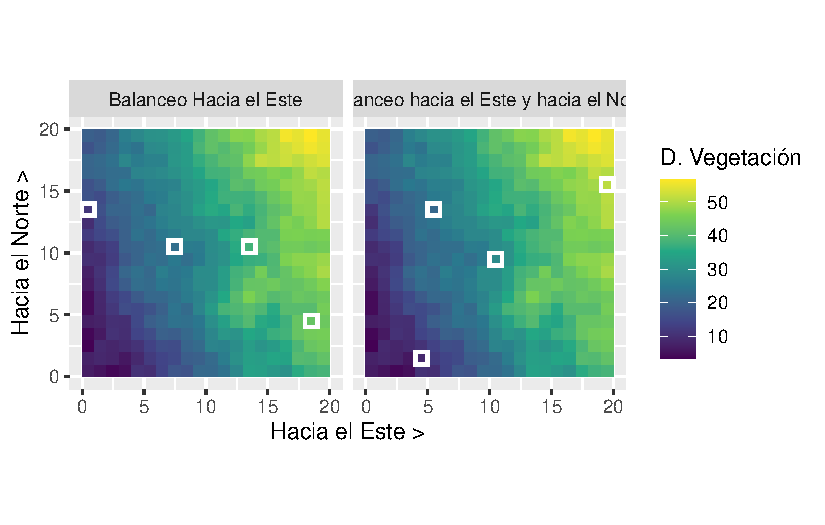
\includegraphics[width=1\linewidth,height=\textheight,keepaspectratio]{cubo_files/figure-pdf/fig-muestreo_cube_ejemplo-1.pdf}

}

\end{figure}%

Por otro lado, en la Figura~\ref{fig-muestreo_cube_ejemplo} también se
observan las 2 muestras balanceadas de la población descritas en el
párrafo anterior. Cada muestra posee 4 casos representados por los
cuadrados blancos. La de la izquierda se encuentra balanceada solamente
por el eje ``Hacia el Este'' y, acorde con esto, los casos seleccionados
se esparcen de Este al Oeste. La muestra de la derecha, en cambio, se
encuentra balanceada por ambos ejes por lo que la distribución de los
casos seleccionados no solo varían de Esta a Oeste, sino que también lo
hacen de Norte a Sur. En este sentido específico, se puede afirmar que
la segunda muestra es más balanceada que la primera y, de manera
intuitiva, se puede afirmar que aquella es más representativa que esta.

\section{Muestras Balanceadas sobre base de
establecimientos}\label{sec-cubo-establecimientos}

Ahora pasaremos a aplicar este diseño a la base de escuelas que venimos
trabajando. Esta vez vamos a incorporar una mayor cantidad de
información secundaria que se encuentra disponible en la base de
establecimientos. Como en muchas otras técnicas, la introducción de más
variables no es garantía de un mejor resultado, ya que en este caso la
agregación de más variables, especialmente si no están linealmente
relacionadas con las variables de estudio, puede ser contraproducente
(Tillé 2011, pág. 222). Ese es precisamente una de las utilidades del
ejemplo anterior de la Figura~\ref{fig-muestreo_cube_ejemplo}, ya que en
él era fácil construir y visualizar la linealidad de la relación entre
las covariables y la variable de estudio. Por esta razón, en este
proceso de selección es clave tener claras las variables de estudio,
para luego determinar qué covariables de la información secundaria
disponible es conveniente incluir.

En este caso, nos focalizaremos en diferentes tipos de objetivos para
demostrar la flexibilidad de la técnica. En primer lugar, nos interesará
tener una muestra de los establecimientos desde la base de los
establecimientos (Sección~\ref{sec-cubo_colegios}) y luego una muestra
de los estudiantes desde esa misma base
(Sección~\ref{sec-cubo_estudiantes}).

Las lista de covariables que serán incluidas, con fines más
metodológicos que teóricos, serán las siguientes:

\begin{itemize}
\item
  Matrícula
\item
  Secciones
\item
  Región
\item
  Ámbito
\end{itemize}

\noindent La lista anterior funciona a modo de ejemplo aunque tiene la
virtud de trabajar con información secundaria casi completa, ya que se
trata de variables con muy baja tasa de no respuesta. En efecto, aquí
usaremos estas covariables tanto cuando nos interese averiguar
características de los establecimientos como de los estudiantes, pero un
análisis más real implicaría usar un conjunto diferente para cada
muestra. La razón de esto es al ser diferentes las variables de estudio
también podrían/deberían ser las covariables disponibles y/o usadas.

Dicho lo anterior parece pertinente el siguiente comentario. Cuando
algunos establecimientos no tienen datos en algunas de las covariables
utilizadas estos no forman parte de la muestra. Esto recuerda algo que
se había comentado cuando se vio el muestreo por azar simple
(Sección~\ref{sec-azar_simple}). El muestreo por azar simple solo exige
una lista (y/o algún dato que luego permita su contacto empírico) de los
miembros de la población. El método del cubo exige, además, el acceso a
otras variables de la población en cuestión en forma de información
auxiliar. Si existen casos que no tienen esa información, estos no
podrán ingresar a la muestra y esto tiene diferentes tipos de
consecuencias.

La primera consecuencia es que el investigador se puede enfrentar a la
disyuntiva sobre si se prefiere a) usar covariables completas (en el
sentido que no tienen casos faltantes) pero con una menor relación con
la/s variable/s de estudio o si se prefiere b) covariables incompletas
pero más fuertemente relacionadas con estas últimas. Siempre pensando en
casos algo extremos, en el primer caso el balanceo será efectivo, pero
quizá contraproducente porque balanceará la muestra con variables que no
se encuentran empíricamente relacionadas con la variable de estudio. En
el segundo caso se aumentan los problemas de cobertura
(\emph{undercoverage error}) y se disminuye la precisión de la muestra
por trabajar con menos casos.

Para poner un ejemplo, las variables ``sondeo\_primero'' y
``sondeo\_segundo'' podrían ser opciones como covariables (siempre igual
dependiendo de que se quiera investigar) pero tienen una alta tasa de no
respuesta o de dato faltante (+ de 550 casos). Y parece ser que esta
ausencia de datos se distribuye de manera desigual entre la población de
los establecimientos, ya que los mismos se concentran en
establecimientos con una matrícula de menos de 10 estudiantes. En este
caso su uso como covariables generaría un sesgo (\emph{bias}) muestral
por el problema de la falta de cobetura porque los casos que integran la
muestra (p.e. Ámbito Urbano) son diferentes a los que no integran (p.e.
Ámbitos Rurales). En otras palabras, la ausencia de datos no es
aleatoria por lo que los van a quedar dentro de la muestra serán, por
diseño, diferentes a los que quedaran fuera de la misma.\footnote{En
  este sentido, más que nada por razones pedagógicas, aquí se han
  elegido como covariables, un conjunto de variables con poco margen de
  no respuesta. Esto se debe a que, si se hubieran escogido covariables
  con una alta tasa de no respuesta, se presenta el problema de contra
  que conjunto de datos testear las bondades de la técnica del balanceo.
  Esto es así dado que si los resultados de la técnica del cubo se
  comparan contra los totales poblacionales de los colegios
  (Tabla~\ref{tbl-parametros_base}) es esperable que los resultados
  vayan a ser diferentes porque, estrictamente, el balanceo se realiza
  solo sobre los establecimientos que tienen la información auxiliar
  pertinente. Lo mismo, \emph{mutatis mutandis}, si se compara la
  técnica del balanceo con la respectiva muestra de azar simple de toda
  la población de colegios (Tabla~\ref{tbl-azar_simple}).}

\subsection{Muestra Balanceada - Población
Establecimientos}\label{sec-cubo_colegios}

En esta primera aplicación del muestreo del cubo con la base de
establecimientos vamos a tener como objetivo tener una muestra de la
población de establecimientos y no, por ejemplo, de los estudiantes. En
el primer caso, en principio, las probabilidades de inclusión son
iguales para cada establecimiento. Como veremos más adelante
(Sección~\ref{sec-cubo_estudiantes}) esta técnica también permite
realizar muestras con diferentes probabilidades de inclusión.

En la Tabla~\ref{tbl-cubo_colegios} se puede observar los resultados de
la muestra balanceada para colegios. En esta tabla los resultados se
comparan contra los resultados anteriores de la muestra de azar simple y
los respectivos totales poblacionales. Como se aclaró anteriormente en
estas tablas no se van a incluir ni el error estándar ni los intervalos
de confianza dada lo incómodo de su cálculo y posterior visualización en
tablas. De todos modos, se alcanza a visualizar que en muchas de las
variables analizadas existe una pequeña mejora con la excepción de
algunas categorías de la variable Región.\footnote{Es posible que parte
  de los mayores sesgos en algunas categorías de la variable Región se
  deban a que la falta de datos en algunas de las covariables elegidas
  sea desigual según Región. De todos modos, la cantidad de casos
  (establecimientos) que no tenían las covariables completas era 9.}

\begin{table}

\caption{\label{tbl-cubo_colegios}Estimaciones con muestra balanceada
para colegios}

\centering{

\fontsize{12.0pt}{14.4pt}\selectfont
\begin{tabular*}{\linewidth}{@{\extracolsep{\fill}}lccc}
\toprule
 & \textbf{Balanceo Colegios} & \textbf{Azar Simple} & \textbf{Pob. Colegios} \\ 
\cmidrule(lr){2-2} \cmidrule(lr){3-3} \cmidrule(lr){4-4}
\textbf{Característica} & \textbf{N = 4.159}\textsuperscript{\textit{1}} & \textbf{N = 4.168}\textsuperscript{\textit{1}} & \textbf{N = 4.168}\textsuperscript{\textit{2}} \\ 
\midrule\addlinespace[2.5pt]
matricula & 269,2 & 276,6 & 267,9 \\ 
secciones & 11,2 & 11,6 & 11,2 \\ 
sondeo\_primero & 57,4 & 56,2 & 57,3 \\ 
    Desconocido & 610 & 472 & 560 \\ 
sondeo\_segundo & 69,1 & 69,8 & 69,5 \\ 
    Desconocido & 638 & 556 & 570 \\ 
region &  &  &  \\ 
    01 & 4,0\% (n=12) & 2,3\% (n=7) & 4,5\% (189) \\ 
    02 & 4,7\% (n=14) & 6,3\% (n=19) & 5,4\% (223) \\ 
    03 & 5,0\% (n=15) & 5,3\% (n=16) & 5,0\% (210) \\ 
    04 & 4,0\% (n=12) & 7,0\% (n=21) & 5,1\% (213) \\ 
    05 & 3,7\% (n=11) & 2,7\% (n=8) & 4,7\% (194) \\ 
    06 & 3,3\% (n=10) & 3,7\% (n=11) & 3,6\% (148) \\ 
    07 & 2,7\% (n=8) & 3,7\% (n=11) & 3,3\% (138) \\ 
    08 & 3,7\% (n=11) & 5,3\% (n=16) & 3,6\% (149) \\ 
    09 & 5,0\% (n=15) & 6,7\% (n=20) & 4,9\% (205) \\ 
    10 & 6,0\% (n=18) & 6,7\% (n=20) & 5,4\% (224) \\ 
    11 & 6,0\% (n=18) & 4,3\% (n=13) & 4,0\% (166) \\ 
    12 & 4,3\% (n=13) & 2,3\% (n=7) & 3,7\% (155) \\ 
    13 & 3,0\% (n=9) & 2,7\% (n=8) & 3,1\% (131) \\ 
    14 & 5,0\% (n=15) & 4,0\% (n=12) & 4,1\% (169) \\ 
    15 & 3,7\% (n=11) & 3,3\% (n=10) & 4,2\% (174) \\ 
    16 & 5,3\% (n=16) & 2,0\% (n=6) & 3,0\% (125) \\ 
    17 & 6,0\% (n=18) & 3,3\% (n=10) & 3,2\% (133) \\ 
    18 & 4,3\% (n=13) & 3,0\% (n=9) & 3,8\% (160) \\ 
    19 & 2,7\% (n=8) & 2,7\% (n=8) & 2,8\% (118) \\ 
    20 & 2,3\% (n=7) & 3,7\% (n=11) & 3,8\% (159) \\ 
    21 & 3,3\% (n=10) & 2,0\% (n=6) & 2,8\% (117) \\ 
    22 & 3,3\% (n=10) & 4,0\% (n=12) & 3,7\% (153) \\ 
    23 & 3,0\% (n=9) & 4,7\% (n=14) & 3,7\% (153) \\ 
    24 & 4,0\% (n=12) & 3,0\% (n=9) & 4,7\% (196) \\ 
    25 & 1,7\% (n=5) & 5,3\% (n=16) & 4,0\% (166) \\ 
ambito &  &  &  \\ 
    Urbano & 64,0\% (n=192) & 67,0\% (n=201) & 65,4\% (2.727) \\ 
    Rural Disperso & 28,7\% (n=86) & 20,3\% (n=61) & 25,7\% (1.073) \\ 
    Rural Agrupado & 7,3\% (n=22) & 12,7\% (n=38) & 8,8\% (368) \\ 
    Desconocido &  &  & 9 \\ 
    Desconocido &  &  & 9 \\ 
\bottomrule
\end{tabular*}
\begin{minipage}{\linewidth}
\textsuperscript{\textit{1}}Media (DE); \% (n sin ponderar)\\
\textsuperscript{\textit{2}}Media; \% (n)\\
\end{minipage}

}

\end{table}%

\subsection{Muestra Balanceada - Población
Estudiantes}\label{sec-cubo_estudiantes}

En esta pequeña sección vamos a observar la flexibilidad de la técnica
del cubo obteniendo una muestra en donde las probabilidades de inclusión
son diferentes. En este caso particular se aplicará el criterio que esas
probabilidades sean proporcionales al tamaño de la matrícula aunque,
claro está, esas probabilidades de inclusión diferentes podrían ser
diferentes. Por ejemplo, se podría especificar que en una muestra tipo
panel, que los establecimientos que entraron en la muestra el año pasado
tengan más chances de (volver a) entrar en la misma. Esto tiene
consecuencias similares a lo visto en el muestreo PPS
(Sección~\ref{sec-pps}) en donde, por diseño, los establecimientos con
mayor matrícula tienen una mayor chance de ser incluidos en la muestra.
La diferencia con el muestreo PPS es que el muestreo balanceado permite,
además, un trabajar con un conjunto de otras covariables que,
nuevamente, reducen las chances que la muestra finalmente seleccionada
sean una de las pocas (muy) sesgadas.

A continuación, en la Tabla~\ref{tbl-cubos_matricula_comparacion} puede
observarse como esta muestra tiene resultados aceptables en cuanto a su
cercanía con los respectivos parámetros poblacionales (que fueron
ponderados por el valor de la matrícula). En cuanto a su comparación con
la muestra PPS sin ponderar no parece registrarse mejoras sustanciales
dado que, por azar, la muestra PPS ya era lo suficientemente buena. La
diferencia es que la técnica de balanceo, gracias al algoritmo del cubo,
\textbf{asegura} que que no saldrá una mala muestra mientras que con el
PPS se trata de confiar en que uno no tendrá mala suerte para que, por
azar, se produzca una mala muestra.

\begin{table}

\caption{\label{tbl-cubos_matricula_comparacion}Comparación muestra
balanceada por la matrícula y muestra PPS sin ponderar y poblacion de
establecimientos ponderada por matrícula}

\centering{

\fontsize{12.0pt}{14.4pt}\selectfont
\begin{tabular*}{\linewidth}{@{\extracolsep{\fill}}lccc}
\toprule
 & \textbf{Cubo Matrícula} & \textbf{PPS sin ponderar} & \textbf{Pob. matricula} \\ 
\cmidrule(lr){2-2} \cmidrule(lr){3-3} \cmidrule(lr){4-4}
\textbf{Característica} &  &  &  \\ 
\midrule\addlinespace[2.5pt]
matricula & 524,4 & 529,5 & 524,2 \\ 
secciones & 19,7 & 19,7 & 19,6 \\ 
sondeo\_primero & 54,0 & 54,1 & 53,8 \\ 
sondeo\_segundo & 68,0 & 67,9 & 67,7 \\ 
region &  &  &  \\ 
    01 & 6,3\% (n=19) & 6,3\% (n=19) & 5,8\% (n=189) \\ 
    02 & 8,7\% (n=26) & 7,0\% (n=21) & 7,9\% (n=222) \\ 
    03 & 8,7\% (n=26) & 9,7\% (n=29) & 9,9\% (n=210) \\ 
    04 & 9,3\% (n=28) & 13,7\% (n=41) & 9,2\% (n=213) \\ 
    05 & 10,7\% (n=32) & 7,0\% (n=21) & 9,5\% (n=194) \\ 
    06 & 2,3\% (n=7) & 3,7\% (n=11) & 4,2\% (n=148) \\ 
    07 & 4,0\% (n=12) & 2,7\% (n=8) & 3,7\% (n=138) \\ 
    08 & 6,0\% (n=18) & 5,7\% (n=17) & 6,1\% (n=149) \\ 
    09 & 10,0\% (n=30) & 11,3\% (n=34) & 10,5\% (n=204) \\ 
    10 & 2,7\% (n=8) & 5,0\% (n=15) & 4,1\% (n=221) \\ 
    11 & 9,0\% (n=27) & 5,0\% (n=15) & 6,3\% (n=166) \\ 
    12 & 2,7\% (n=8) & 2,0\% (n=6) & 2,4\% (n=155) \\ 
    13 & 1,3\% (n=4) & 1,3\% (n=4) & 1,5\% (n=131) \\ 
    14 & 1,0\% (n=3) & 3,0\% (n=9) & 1,7\% (n=169) \\ 
    15 & 1,3\% (n=4) & 2,3\% (n=7) & 1,7\% (n=172) \\ 
    16 & 1,0\% (n=3) & 0,0\% (n=0) & 0,9\% (n=125) \\ 
    17 & 1,0\% (n=3) & 0,7\% (n=2) & 0,8\% (n=133) \\ 
    18 & 2,0\% (n=6) & 3,7\% (n=11) & 2,0\% (n=160) \\ 
    19 & 2,0\% (n=6) & 1,3\% (n=4) & 2,9\% (n=118) \\ 
    20 & 1,0\% (n=3) & 1,3\% (n=4) & 1,8\% (n=159) \\ 
    21 & 1,0\% (n=3) & 1,3\% (n=4) & 0,9\% (n=117) \\ 
    22 & 4,3\% (n=13) & 2,3\% (n=7) & 2,8\% (n=153) \\ 
    23 & 1,3\% (n=4) & 1,3\% (n=4) & 0,9\% (n=151) \\ 
    24 & 0,7\% (n=2) & 0,7\% (n=2) & 1,1\% (n=196) \\ 
    25 & 1,7\% (n=5) & 1,7\% (n=5) & 1,4\% (n=166) \\ 
ambito &  &  &  \\ 
    Urbano & 96,3\% (n=289) & 95,3\% (n=286) & 96,1\% (n=2.723) \\ 
    Rural Disperso & 1,3\% (n=4) & 1,7\% (n=5) & 1,9\% (n=1.070) \\ 
    Rural Agrupado & 2,3\% (n=7) & 3,0\% (n=9) & 2,1\% (n=366) \\ 
\bottomrule
\end{tabular*}

}

\end{table}%

\section{Muestreos bien distribuidos}\label{sec-bien_distribuido}

Como se dijo en la Sección~\ref{sec-cubo}, en los muestreos balanceados
por el método del cubo el esfuerzo está en que los valores de la
tendencia central de los estimadores de determinadas variables de la
muestra se acerquen a los valores de \textbf{tendencia central} de las
covariables existentes como información secundaria, esto es, a los
parámetros conocidos de la población. En el muestreo bien distribuido o
bien extendido (\emph{well spread}) es objetivo es similar pero con una
restricción adicional que implica que \textbf{la distribución} de la/s
covariable/s de la muestra se acerque a la distribución de la/s
covariable/s en la población. El precio de esta mejora es que se debe
conocer la distribución de esas variables en la población algo que,
hasta ahora, nunca habían requerido los diseños anteriores. En el caso
particular de la distribución espacial el diseño exige la introducción
de las coordenadas de cada miembro de la población y no solo el promedio
poblacional de ellas.

En este contexto cobra importancia el ejemplo inicial de la
Figura~\ref{fig-muestreo_cube_ejemplo} en donde se usaron covariables
espaciales. Allí, de manera intuitiva, se asoció que una muestra bien
distribuida es una muestra balanceada. Esta afirmación, útil como un
primera aproximación, es verdadera pero su inversa no. En otras
palabras, toda muestra balanceada no es, necesariamente, una muestra
bien distribuida, pero toda muestra bien distribuida sí es,
necesariamente, una muestra balanceada.

A continuación trabajaremos con los misma muestra balanceada de colegios
de la sección anterior pero le agregaremos la condición de que esa
muestra \emph{también} sea bien distribuida en los valores de las
coordenadas geográficas de los establecimientos. Para eso primero
agregaremos las coordenadas a la base de los establecimientos y luego
nos quedaremos con sólo aquellos establecimientos que tengan las
coordenadas.

Agregadas las coordenadas ahora se puede aplicar la técnica del cubo con
el adicional que el balanceo no sólo se realice por los valores de
tendencia central de la sección anterior, sino también con los valores
de dispersión de las coordenadas de los establecimientos.

En cierto sentido, la inclusión de las variables ``Ámbito'' y ``Región''
en el diseño balanceado (Sección~\ref{sec-cubo_colegios}) ya mejoraban
la distribución geográfica o espacial de la muestra (con respecto a una
muestra de azar simple) pero lo hacían focalizándose en sus valores de
tendencia central. Los valores de las coordenadas permiten una
información de un grano más fino sobre la distribución espacial de la
muestra lo que no es un dato menor. Si se asume que el espacio es una
especie de meta-variable en las ciencias sociales (Small y Adler 2019),
controlar la muestra por el espacio ayuda a controlar una serie de otras
características que poseen eficacia causal pero, usualmente son
inobservables o de difícil registro. Expresado en la jerga del diseño
estadístico de las investigaciones, este tipo de mejoras ayudan a que
dentro del conjunto de variables extrañas al comienzo de la
investigación, gracias al diseño de la misma, pasen ser variables
controladas en vez de pasar a ser variables perturbadoras (Kish 1987).
De todos modos, cabe destacar que las coordenadas son de los
establecimientos y no de los estudiantes o, más en general, de las
personas. El supuesto implícito es que la ubicación de los
establecimientos guarda una relación estrecha con la ubicación de los
estudiantes.

Desde un costado más operativo el algoritmo que se utiliza es el
algoritmo del ``\emph{local cube}'' (Tillé y Grafström 2013) que ya
había sido utilizado en el muestro PPS. Este algoritmo penaliza si se
seleccionan 2 casos ``localmente'' cercanos entre sí y luego de haber
seleccionado un caso hay pocas chances que se seleccione otro caso muy
cercano. La idea de distancia entre los casos es abstracta aunque en
nuestro ejemplo se puede interpretar como distancia espacial.

\begin{table}

\caption{\label{tbl-bien_distribuida}Comparación entre muestra bien
distribuida, balanceada y población de establecimientos}

\centering{

\fontsize{12.0pt}{14.4pt}\selectfont
\begin{tabular*}{\linewidth}{@{\extracolsep{\fill}}lccc}
\toprule
 & \textbf{Bien distribuida} & \textbf{Balanceo colegios} & \textbf{Pob. Colegios} \\ 
\cmidrule(lr){2-2} \cmidrule(lr){3-3} \cmidrule(lr){4-4}
\textbf{Característica} & \textbf{N = 4.156}\textsuperscript{\textit{1}} & \textbf{N = 4.159}\textsuperscript{\textit{1}} & \textbf{N = 4.168}\textsuperscript{\textit{2}} \\ 
\midrule\addlinespace[2.5pt]
matricula & 268,0 (2,8) & 269,2 & 267,9 \\ 
secciones & 11,1 (0,1) & 11,2 & 11,2 \\ 
sondeo\_primero & 58,0 (0,2) & 57,4 & 57,3 \\ 
sondeo\_segundo & 68,5 (0,2) & 69,1 & 69,5 \\ 
region &  &  &  \\ 
    01 & 4,3\% (n=13) & 4,0\% (n=12) & 4,5\% (189) \\ 
    02 & 5,7\% (n=17) & 4,7\% (n=14) & 5,4\% (223) \\ 
    03 & 5,0\% (n=15) & 5,0\% (n=15) & 5,0\% (210) \\ 
    04 & 5,0\% (n=15) & 4,0\% (n=12) & 5,1\% (213) \\ 
    05 & 4,3\% (n=13) & 3,7\% (n=11) & 4,7\% (194) \\ 
    06 & 3,7\% (n=11) & 3,3\% (n=10) & 3,6\% (148) \\ 
    07 & 3,3\% (n=10) & 2,7\% (n=8) & 3,3\% (138) \\ 
    08 & 3,7\% (n=11) & 3,7\% (n=11) & 3,6\% (149) \\ 
    09 & 5,3\% (n=16) & 5,0\% (n=15) & 4,9\% (205) \\ 
    10 & 5,3\% (n=16) & 6,0\% (n=18) & 5,4\% (224) \\ 
    11 & 3,7\% (n=11) & 6,0\% (n=18) & 4,0\% (166) \\ 
    12 & 4,0\% (n=12) & 4,3\% (n=13) & 3,7\% (155) \\ 
    13 & 2,7\% (n=8) & 3,0\% (n=9) & 3,1\% (131) \\ 
    14 & 3,7\% (n=11) & 5,0\% (n=15) & 4,1\% (169) \\ 
    15 & 5,0\% (n=15) & 3,7\% (n=11) & 4,2\% (174) \\ 
    16 & 2,3\% (n=7) & 5,3\% (n=16) & 3,0\% (125) \\ 
    17 & 3,7\% (n=11) & 6,0\% (n=18) & 3,2\% (133) \\ 
    18 & 3,7\% (n=11) & 4,3\% (n=13) & 3,8\% (160) \\ 
    19 & 3,0\% (n=9) & 2,7\% (n=8) & 2,8\% (118) \\ 
    20 & 3,3\% (n=10) & 2,3\% (n=7) & 3,8\% (159) \\ 
    21 & 3,3\% (n=10) & 3,3\% (n=10) & 2,8\% (117) \\ 
    22 & 4,0\% (n=12) & 3,3\% (n=10) & 3,7\% (153) \\ 
    23 & 4,0\% (n=12) & 3,0\% (n=9) & 3,7\% (153) \\ 
    24 & 4,7\% (n=14) & 4,0\% (n=12) & 4,7\% (196) \\ 
    25 & 3,3\% (n=10) & 1,7\% (n=5) & 4,0\% (166) \\ 
ambito &  &  &  \\ 
    Urbano & 65,0\% (n=195) & 64,0\% (n=192) & 65,4\% (2.727) \\ 
    Rural Disperso & 26,7\% (n=80) & 28,7\% (n=86) & 25,7\% (1.073) \\ 
    Rural Agrupado & 8,3\% (n=25) & 7,3\% (n=22) & 8,8\% (368) \\ 
    Desconocido &  & 610 & 560 \\ 
    Desconocido &  & 638 & 570 \\ 
    Desconocido &  &  & 9 \\ 
    Desconocido &  &  & 9 \\ 
\bottomrule
\end{tabular*}
\begin{minipage}{\linewidth}
\textsuperscript{\textit{1}}Media (DE); \% (n sin ponderar)\\
\textsuperscript{\textit{2}}Media; \% (n)\\
\end{minipage}

}

\end{table}%

Como puede observarse en Tabla~\ref{tbl-bien_distribuida}, al usarse la
distribución de las coordenadas como covariables se aprecia una leve
mejora en los valores que tienen una fuerte influencia espacial (p.e
``Ambito'' y ``Región''). Sin embargo, una manera más visual de captar
esta mejora es, al igual que en la
Figura~\ref{fig-muestreo_cube_ejemplo}, a través de un mapa como el de
la \textbf{?@fig-mapa\_bien\_distribuida} .

\begin{figure}

\caption{\label{fig-mapa_bien_distribuida_pdf}Distribución de la
población de los establecimientos (puntos negros) y de la muestra bien
distribuida (puntos azules)}

\centering{

\pandocbounded{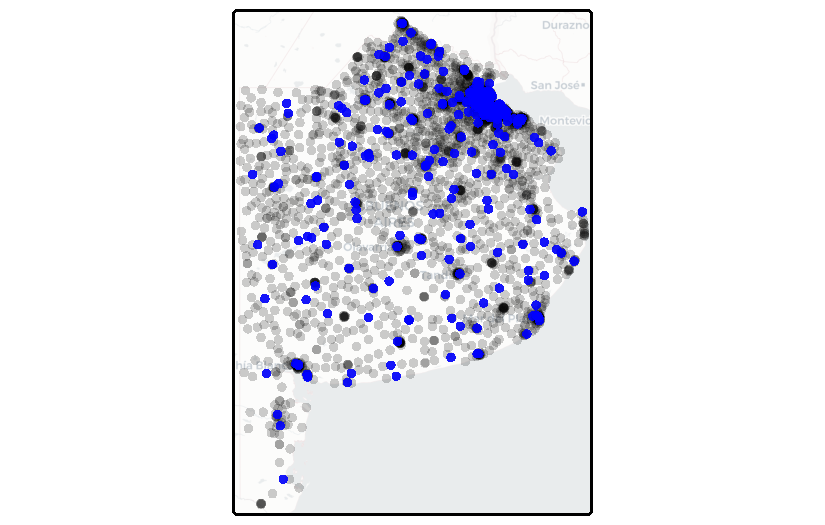
\includegraphics[keepaspectratio]{cubo_files/figure-pdf/fig-mapa_bien_distribuida_pdf-1.pdf}}

}

\end{figure}%

\bookmarksetup{startatroot}

\chapter{Calibración}\label{sec-calibracion}

La estrategia de la calibración está compuesta por un conjunto de
prácticas que aspiran a lograr objetivos similares al proceso del
balanceo del cubo pero con métodos cualitativamente diferentes. La
principal diferencia radica en que la calibración se realiza
\emph{ex-post} la ejecución de la muestra (o sea, en el momento de la
estimación) y no \emph{ex-ante} (o sea, en el momento del diseño)
(Deville y Tillé 2004, pág. 907). Esto es una diferencia fundamental que
emparenta a la calibración con el enfoque del ``\emph{Model Assisted}''
y la aleja del ``\emph{Design Based}''\footnote{En cambio el balanceo,
  si bien en su origen tiene una fuerte vinculación con el enfoque del
  ``Model Assisted'', no se encuentra tan alejado del ``design based''
  dado que el algoritmo del cubo selecciona muestras balanceadas dentro
  del conjunto de muestras aleatorias (Tillé 2010, pág. 39).}. En
efecto, tanto el balanceo como la calibración pueden considerarse
prácticas relativamente generales que, en su interior, incluyen otras
prácticas más específicas. Esto es lo que habilita a afirmar que, por
ejemplo, la estratificación es un caso particular del balanceo así como
la post-estratificación es un caso particular de la calibración (Tillé
2011, pág. 223).

Otra diferencia entre el balanceo y la calibración es que para realizar
la calibración en algunas situaciones (esto depende de la técnica
específica seleccionada) solo es necesario los totales de la población y
no, como en el balanceo, los valores de cada unidad que compone esa
población.

Las características anteriores hacen que el proceso de calibración sea
muy útil en momentos en donde existe conocimientos sobre algunos totales
de la población y no se haya podido controlar mucho el proceso de diseño
de la muestra (p.e. diseños no probabilistas) o diseños probabilistas
pero con una alta tasa de no respuesta. Estas características hacen al
proceso de calibración algo muy deseado para muchas investigaciones
contemporáneas en donde pueda admitirse que se conocen algunos
parámetros poblacionales y, por ejemplo, se ha realizado una muestra que
se difundió de manera virtual a través de un link que circuló por
diferentes redes sociales. Esto deja en pie la discusión sobre que ``tan
buenos'' podrán ser los resultados de esa investigación, pero no parece
haber muchas dudas que la investigación del ejemplo anterior será mejor
si se le realiza un proceso de calibración mientras que será peor si no
se realiza ese proceso.\footnote{Este tipo de discusiones ha enfrentado
  (y por ahora continúa enfrentando) a los representantes de los
  enfoques de la ``\emph{design based sample}'' y del ``\emph{model
  assisted}''. Los primeros suelen dudar de los beneficios de aplicar la
  calibración sobre diseños no probabilísticos aunque no suelen tener
  objeciones cuando la calibración se realiza sobre diseños
  probabilísticos (Elliott y Valliant 2017). En el fondo lo que está en
  juego son los grados de garantía que ofrece cada técnica acerca de la
  representatividad y esto no solo incluya la discusión sobre las
  heterogeneidades observables (algo mantenido por ambos enfoques) sino
  también sobre las heterogeneidades no observables (algo históricamente
  mantenido por el enfoque de la ``\emph{design}'').}

En cuanto a su pertinencia, siempre que haya disponibilidad de tiempo (y
el saber necesario para realizarlo) es aconsejable realizar una
calibración. Esto es cierto al menos porque el balanceo tiene el
problema del redondeo (las muestras son muestras de números enteros) y
la calibración no, ya que puede construirse calibradores con números
racionales. Por esta misma razón, aun cuando se haya realizado una
muestra con un diseño por balanceo, es recomendable calibrar con los
totales de las variables que se usaron en el proceso de balanceo.

Detalladas algunas diferencias entre la calibración y el balanceo ahora
se pasa a diferenciar la calibración (de una muestra) de la imputación
(de variables específicas).

\begin{itemize}
\item
  En cuanto a su producto, la calibración produce como resultado un
  calibrador (o un nuevo ponderador en la situación que el diseño de la
  muestra ya cuente con un ponderador) que es único para cada caso
  seleccionado en la muestra. En cambio la imputación, al menos como acá
  se la está entendiendo, es un proceso que tiene como objetivo estimar
  el valor faltante de una variable de los casos que respondieron de
  forma incompleta la muestra. En este sentido, un caso efectivamente
  seleccionado en la muestra puede tener más un valor imputado (p.e.
  para la variable ingresos y para la variable autopercepción de género)
  y, en cambio, otro caso puede que no tenga ninguno (p.e. si ese caso
  tuvo respuestas en todas las variables). En otros contextos se suele
  diferenciar a ambos procesos afirmando que la calibración ayuda a
  mitigar el problema del \emph{unit-not-response} y la imputación ayuda
  a mitigar el problema del \emph{ítem-not-response} {[}Lumley (2010),
  pág. 136{]}(Lundström y Särndal 2009, pág. 9).
\item
  En cuanto a los insumos, la calibración necesita los totales
  poblacionales y, en cambio, la imputación necesita los valores de las
  otras variables que el caso a imputar ha respondido así como los
  valores de las covariables y la variable a imputar de los otros casos.
\item
  En cuanto al momento de la investigación, siempre que se usen ambos
  procesos, usualmente primero se imputa los casos particulares de las
  variables que se considera pertinente y luego se calibra la muestra
  incluyendo los valores de los casos imputados. Este orden es
  particularmente importante si se confía en el proceso de la imputación
  y la/s variable/s imputadas son parte del proceso de calibración como
  covariables.
\end{itemize}

\noindent Por último, a veces se suele asimilar como sinónimos en
término calibración con el término post-estratificación. Más arriba ya
se había comentado que el segundo puede considerarse como un caso
particular (aunque quizás el más difundido) del primero en donde solo se
utilizan variables categóricas (estratos) para el proceso de la
calibración. Lo mismo puede afirmarse del método menos difundido del
``raking'' que permite la calibración de múltiples variables categóricas
sin la necesidad de realizar cruces entre ellas con el riesgo de no
tener casos en la muestra de algunas de las celdas de los múltiples
cruces (Lumley 2010, pág. 139). Por esta razón, aquí usaremos
directamente el método de la calibración por ser el más general, ya que
permite la inclusión tanto de variables categóricas como continuas y no
presenta los riesgos de la post-calibración en cuanto a la posible
ausencia de casos frutos de los cruces de las variables categóricas.

A continuación vamos a trabajar con 2 ejemplos alternativos. Uno, en
donde la calibración se realiza sobre la muestra aleatoria simple y otra
que se realiza sobre la muestra balanceada y bien distribuida. En
función de lo visto anteriormente (Sección~\ref{sec-azar_simple},
Sección~\ref{sec-cubo} y Sección~\ref{sec-bien_distribuido}) ya sabemos
que ambas calibraciones van a partir desde un punto de inicio diferente.
Veremos que tanta distancia entre sí y con respecto a los parámetros
poblaciones van a tener los respectivos puntos de llegada (esto es, las
estimaciones de ambas muestras) luego de realizar la calibración. En
otras palabras, la muestra balanceada y bien distribuida ya se
encontraba (en general) bastante cerca de los parámetros poblacionales
por lo que, a priori, cuenta con alguna ventaja desde su puesto de
largada.

\section{Calibración muestra azar
simple}\label{calibraciuxf3n-muestra-azar-simple}

Comenzaremos haciendo la calibración sobre nuestra muestra realizada por
azar simple y su resultado lo comparemos con la respectiva muestra de
azar simple (sin calibrar) y con los respectivos parámetros
poblacionales. Vamos a ver que, en comparación con otras técnicas, la
mayor flexibilidad de la calibración se paga con una mayor
especificación de los parámetros de sus funciones\footnote{En otras
  palabras, si ya se sabe de antemano que se va a realizar una
  post-estratificación es más simple utilizar una función específica
  para post-estratificar (p.e. la función ``poststratify'' de la
  librería survey o ``poststrata'' de la librería sampling).}.

Para eso vamos a recuperar el objeto con el cual le informábamos a R que
habíamos realizado una muestra aleatoria simple
(Sección~\ref{sec-azar_simple}). Ese va a ser nuestro primer insumo al
cual le vamos a realizar la calibración y para eso es importante el
proceso de la selección y armado de las covariables. Esta parte es
similar en espíritu a lo realizado en el proceso de balanceo, pero la
parte operativa tiene pequeñas diferencias como se observa en el
siguiente código.

\begin{verbatim}
Sample:  [1] "(Intercept)"          "matricula"            "ambitoRural Disperso"
 [4] "ambitoRural Agrupado" "region02"             "region03"            
 [7] "region04"             "region05"             "region06"            
[10] "region07"             "region08"             "region09"            
[13] "region10"             "region11"             "region12"            
[16] "region13"             "region14"             "region15"            
[19] "region16"             "region17"             "region18"            
[22] "region19"             "region20"             "region21"            
[25] "region22"             "region23"             "region24"            
[28] "region25"            
Popltn:  [1] ""  ""  "n" "n" "n" "n" "n" "n" "n" "n" "n" "n" "n" "n" "n" "n" "n" "n" "n"
[20] "n" "n" "n" "n" "n" "n" "n" "n" "n"
\end{verbatim}

\begin{table}

\caption{\label{tbl-azar_simple_calibrado}Calibración muestra azar
simple}

\centering{

\fontsize{12.0pt}{14.4pt}\selectfont
\begin{tabular*}{\linewidth}{@{\extracolsep{\fill}}lccccc}
\toprule
 & \multicolumn{2}{c}{AS Calibrado} & \multicolumn{2}{c}{AS sin calibrar} & Poblacion \\ 
\cmidrule(lr){2-3} \cmidrule(lr){4-5} \cmidrule(lr){6-6}
\textbf{Característica} & \textbf{N = 4.168}\textsuperscript{\textit{1}} & \textbf{95\% CI} & \textbf{N = 4.168}\textsuperscript{\textit{1}} & \textbf{95\% CI} & \textbf{N = 4.168}\textsuperscript{\textit{2}} \\ 
\midrule\addlinespace[2.5pt]
matricula & 267 (0) & 267, 267 & 276,6 (2,9) & 271, 282 & 267,9 \\ 
secciones & 11 (0) & 11, 11 & 11,6 (0,1) & 11, 12 & 11,2 \\ 
sondeo\_primero & 57 (0) & 56, 57 & 56,2 (0,2) & 56, 57 & 57,3 \\ 
    Desconocido & 568 &  & 472 &  & 560 \\ 
sondeo\_segundo & 70 (0) & 69, 70 & 69,8 (0,2) & 69, 70 & 69,5 \\ 
    Desconocido & 647 &  & 556 &  & 570 \\ 
region &  &  &  &  &  \\ 
    01 & 4,5\% (n=7) & 4,5\%, 4,5\% & 2,3\% (n=7) & 2,0\%, 2,7\% & 4,5\% (189) \\ 
    02 & 5,4\% (n=19) & 5,4\%, 5,4\% & 6,3\% (n=19) & 5,8\%, 6,9\% & 5,4\% (223) \\ 
    03 & 5,0\% (n=16) & 5,0\%, 5,0\% & 5,3\% (n=16) & 4,9\%, 5,8\% & 5,0\% (210) \\ 
    04 & 5,1\% (n=21) & 5,1\%, 5,1\% & 7,0\% (n=21) & 6,5\%, 7,6\% & 5,1\% (213) \\ 
    05 & 4,7\% (n=8) & 4,7\%, 4,7\% & 2,7\% (n=8) & 2,3\%, 3,0\% & 4,7\% (194) \\ 
    06 & 3,6\% (n=11) & 3,6\%, 3,6\% & 3,7\% (n=11) & 3,3\%, 4,1\% & 3,6\% (148) \\ 
    07 & 3,3\% (n=11) & 3,3\%, 3,3\% & 3,7\% (n=11) & 3,3\%, 4,1\% & 3,3\% (138) \\ 
    08 & 3,6\% (n=16) & 3,6\%, 3,6\% & 5,3\% (n=16) & 4,9\%, 5,8\% & 3,6\% (149) \\ 
    09 & 4,9\% (n=20) & 4,9\%, 4,9\% & 6,7\% (n=20) & 6,1\%, 7,2\% & 4,9\% (205) \\ 
    10 & 5,4\% (n=20) & 5,4\%, 5,4\% & 6,7\% (n=20) & 6,1\%, 7,2\% & 5,4\% (224) \\ 
    11 & 4,0\% (n=13) & 4,0\%, 4,0\% & 4,3\% (n=13) & 3,9\%, 4,8\% & 4,0\% (166) \\ 
    12 & 3,7\% (n=7) & 3,7\%, 3,7\% & 2,3\% (n=7) & 2,0\%, 2,7\% & 3,7\% (155) \\ 
    13 & 3,1\% (n=8) & 3,1\%, 3,1\% & 2,7\% (n=8) & 2,3\%, 3,0\% & 3,1\% (131) \\ 
    14 & 4,1\% (n=12) & 4,1\%, 4,1\% & 4,0\% (n=12) & 3,6\%, 4,4\% & 4,1\% (169) \\ 
    15 & 4,2\% (n=10) & 4,2\%, 4,2\% & 3,3\% (n=10) & 3,0\%, 3,7\% & 4,2\% (174) \\ 
    16 & 3,0\% (n=6) & 3,0\%, 3,0\% & 2,0\% (n=6) & 1,7\%, 2,3\% & 3,0\% (125) \\ 
    17 & 3,2\% (n=10) & 3,2\%, 3,2\% & 3,3\% (n=10) & 3,0\%, 3,7\% & 3,2\% (133) \\ 
    18 & 3,8\% (n=9) & 3,8\%, 3,8\% & 3,0\% (n=9) & 2,7\%, 3,4\% & 3,8\% (160) \\ 
    19 & 2,8\% (n=8) & 2,8\%, 2,8\% & 2,7\% (n=8) & 2,3\%, 3,0\% & 2,8\% (118) \\ 
    20 & 3,8\% (n=11) & 3,8\%, 3,8\% & 3,7\% (n=11) & 3,3\%, 4,1\% & 3,8\% (159) \\ 
    21 & 2,8\% (n=6) & 2,8\%, 2,8\% & 2,0\% (n=6) & 1,7\%, 2,3\% & 2,8\% (117) \\ 
    22 & 3,7\% (n=12) & 3,7\%, 3,7\% & 4,0\% (n=12) & 3,6\%, 4,4\% & 3,7\% (153) \\ 
    23 & 3,7\% (n=14) & 3,7\%, 3,7\% & 4,7\% (n=14) & 4,2\%, 5,1\% & 3,7\% (153) \\ 
    24 & 4,7\% (n=9) & 4,7\%, 4,7\% & 3,0\% (n=9) & 2,7\%, 3,4\% & 4,7\% (196) \\ 
    25 & 4,0\% (n=16) & 4,0\%, 4,0\% & 5,3\% (n=16) & 4,9\%, 5,8\% & 4,0\% (166) \\ 
ambito &  &  &  &  &  \\ 
    Urbano & 65\% (n=201) & 65\%, 65\% & 67,0\% (n=201) & 66\%, 68\% & 65,4\% (2.727) \\ 
    Rural Disperso & 26\% (n=61) & 26\%, 26\% & 20,3\% (n=61) & 19\%, 21\% & 25,7\% (1.073) \\ 
    Rural Agrupado & 8,8\% (n=38) & 8,8\%, 8,8\% & 12,7\% (n=38) & 12\%, 13\% & 8,8\% (368) \\ 
    Desconocido &  &  &  &  & 9 \\ 
    Desconocido &  &  &  &  & 9 \\ 
\bottomrule
\end{tabular*}
\begin{minipage}{\linewidth}
\textsuperscript{\textit{1}}Media (SE); \% (n=n (unweighted))\\
\textsuperscript{\textit{2}}Media; \% (n)\\
Abreviacion: CI = Intervalo de confianza\\
\end{minipage}

}

\end{table}%

Como puede observarse en Tabla~\ref{tbl-azar_simple_calibrado} la
calibración ha mejorado sensiblemente la muestra de azar simple en casi
todas las variables, aún en aquellas que no se usaron activamente en la
matriz de calibración. En efecto, en la mayoría de las variables los
valores de la muestra calibrada se acercan mucho a los parámetros
poblacionales.

Un paso adicional que se puede realizar si luego se quiere trabajar en
una planilla de cálculo o, más en general, por fuera de R, es agregar
los respectivos ponderadores del proceso de calibración al objeto para
así tenerlos como una variable más. En este sentido, la base de datos
con los casos seleccionados de la muestras ahora pasaría a tener 2
variables especiales que servirían para el proceso de expansión de la
muestra a la población. Uno, un ponderador que ya existía luego de haber
realizado el azar simple (y que era igual para todos los casos) y otro
recientemente agregado, el calibrador, que es específico para cada caso.

\begin{table}

\caption{\label{tbl-base_muestra_AS_cal}Ponderadores y calibradores.
Base muestra azar simple.}

\centering{

\fontsize{12.0pt}{14.4pt}\selectfont
\begin{tabular*}{\linewidth}{@{\extracolsep{\fill}}rrcrrrr}
\toprule
matricula & secciones & ambito & sondeo\_primero & sondeo\_segundo & pond\_weight & cal\_weight \\ 
\midrule\addlinespace[2.5pt]
100 & 6 & Urbano & 42.46154 & 52.88889 & 13.89333 & 12.51390 \\ 
122 & 6 & Urbano & 57.11538 & 50.27273 & 13.89333 & 14.50510 \\ 
78 & 6 & Urbano & 79.93750 & 75.41667 & 13.89333 & 23.16509 \\ 
\bottomrule
\end{tabular*}

}

\end{table}%

\section{Calibración muestra bien
distribuida}\label{sec-cal_bien_distribuida}

En el caso de la calibración de la muestra bien distribuida el proceso
de calibración es similar con la diferencia que cambia el insumo al cual
se le realiza la calibración. Aquí el código es un poco más simple
porque se reutiliza la matriz de covariables construida para la
calibración de la muestra de azar simple.

\begin{verbatim}
Sample:  [1] "(Intercept)"          "matricula"            "ambitoRural Disperso"
 [4] "ambitoRural Agrupado" "region02"             "region03"            
 [7] "region04"             "region05"             "region06"            
[10] "region07"             "region08"             "region09"            
[13] "region10"             "region11"             "region12"            
[16] "region13"             "region14"             "region15"            
[19] "region16"             "region17"             "region18"            
[22] "region19"             "region20"             "region21"            
[25] "region22"             "region23"             "region24"            
[28] "region25"            
Popltn:  [1] ""  ""  "n" "n" "n" "n" "n" "n" "n" "n" "n" "n" "n" "n" "n" "n" "n" "n" "n"
[20] "n" "n" "n" "n" "n" "n" "n" "n" "n"
\end{verbatim}

\begin{table}

\caption{\label{tbl-bien_distribuida_cal}Calibración muestra bien
distribuida}

\centering{

\fontsize{12.0pt}{14.4pt}\selectfont
\begin{tabular*}{\linewidth}{@{\extracolsep{\fill}}lcccc}
\toprule
 & \multicolumn{2}{c}{BD calibrado} & BD sin calibrar & Poblacion \\ 
\cmidrule(lr){2-3} \cmidrule(lr){4-4} \cmidrule(lr){5-5}
\textbf{Característica} & \textbf{N = 4.168}\textsuperscript{\textit{1}} & \textbf{95\% CI} & \textbf{N = 4.156}\textsuperscript{\textit{2}} & \textbf{N = 4.168}\textsuperscript{\textit{3}} \\ 
\midrule\addlinespace[2.5pt]
matricula & 267 (0) & 267, 267 & 268,0 (2,8) & 267,9 \\ 
secciones & 11 (0) & 11, 11 & 11,1 (0,1) & 11,2 \\ 
sondeo\_primero & 58 (0) & 58, 58 & 58,0 (0,2) & 57,3 \\ 
    Desconocido & 478 &  &  & 560 \\ 
sondeo\_segundo & 69 (0) & 68, 69 & 68,5 (0,2) & 69,5 \\ 
    Desconocido & 543 &  &  & 570 \\ 
region &  &  &  &  \\ 
    01 & 4,5\% (n=13) & 4,5\%, 4,5\% & 4,3\% (n=13) & 4,5\% (189) \\ 
    02 & 5,4\% (n=17) & 5,4\%, 5,4\% & 5,7\% (n=17) & 5,4\% (223) \\ 
    03 & 5,0\% (n=15) & 5,0\%, 5,0\% & 5,0\% (n=15) & 5,0\% (210) \\ 
    04 & 5,1\% (n=15) & 5,1\%, 5,1\% & 5,0\% (n=15) & 5,1\% (213) \\ 
    05 & 4,7\% (n=13) & 4,7\%, 4,7\% & 4,3\% (n=13) & 4,7\% (194) \\ 
    06 & 3,6\% (n=11) & 3,6\%, 3,6\% & 3,7\% (n=11) & 3,6\% (148) \\ 
    07 & 3,3\% (n=10) & 3,3\%, 3,3\% & 3,3\% (n=10) & 3,3\% (138) \\ 
    08 & 3,6\% (n=11) & 3,6\%, 3,6\% & 3,7\% (n=11) & 3,6\% (149) \\ 
    09 & 4,9\% (n=16) & 4,9\%, 4,9\% & 5,3\% (n=16) & 4,9\% (205) \\ 
    10 & 5,4\% (n=16) & 5,4\%, 5,4\% & 5,3\% (n=16) & 5,4\% (224) \\ 
    11 & 4,0\% (n=11) & 4,0\%, 4,0\% & 3,7\% (n=11) & 4,0\% (166) \\ 
    12 & 3,7\% (n=12) & 3,7\%, 3,7\% & 4,0\% (n=12) & 3,7\% (155) \\ 
    13 & 3,1\% (n=8) & 3,1\%, 3,1\% & 2,7\% (n=8) & 3,1\% (131) \\ 
    14 & 4,1\% (n=11) & 4,1\%, 4,1\% & 3,7\% (n=11) & 4,1\% (169) \\ 
    15 & 4,2\% (n=15) & 4,2\%, 4,2\% & 5,0\% (n=15) & 4,2\% (174) \\ 
    16 & 3,0\% (n=7) & 3,0\%, 3,0\% & 2,3\% (n=7) & 3,0\% (125) \\ 
    17 & 3,2\% (n=11) & 3,2\%, 3,2\% & 3,7\% (n=11) & 3,2\% (133) \\ 
    18 & 3,8\% (n=11) & 3,8\%, 3,8\% & 3,7\% (n=11) & 3,8\% (160) \\ 
    19 & 2,8\% (n=9) & 2,8\%, 2,8\% & 3,0\% (n=9) & 2,8\% (118) \\ 
    20 & 3,8\% (n=10) & 3,8\%, 3,8\% & 3,3\% (n=10) & 3,8\% (159) \\ 
    21 & 2,8\% (n=10) & 2,8\%, 2,8\% & 3,3\% (n=10) & 2,8\% (117) \\ 
    22 & 3,7\% (n=12) & 3,7\%, 3,7\% & 4,0\% (n=12) & 3,7\% (153) \\ 
    23 & 3,7\% (n=12) & 3,7\%, 3,7\% & 4,0\% (n=12) & 3,7\% (153) \\ 
    24 & 4,7\% (n=14) & 4,7\%, 4,7\% & 4,7\% (n=14) & 4,7\% (196) \\ 
    25 & 4,0\% (n=10) & 4,0\%, 4,0\% & 3,3\% (n=10) & 4,0\% (166) \\ 
ambito &  &  &  &  \\ 
    Urbano & 65\% (n=195) & 65\%, 65\% & 65,0\% (n=195) & 65,4\% (2.727) \\ 
    Rural Disperso & 26\% (n=80) & 26\%, 26\% & 26,7\% (n=80) & 25,7\% (1.073) \\ 
    Rural Agrupado & 8,8\% (n=25) & 8,8\%, 8,8\% & 8,3\% (n=25) & 8,8\% (368) \\ 
    Desconocido &  &  &  & 9 \\ 
    Desconocido &  &  &  & 9 \\ 
\bottomrule
\end{tabular*}
\begin{minipage}{\linewidth}
\textsuperscript{\textit{1}}Media (SE); \% (n=n (unweighted))\\
\textsuperscript{\textit{2}}Media (DE); \% (n sin ponderar)\\
\textsuperscript{\textit{3}}Media; \% (n)\\
Abreviacion: CI = Intervalo de confianza\\
\end{minipage}

}

\end{table}%

Al igual que con la calibración de la base de la muestra de azar simple,
aquí vamos a extraer los calibradores para luego agregarlos a la base de
datos.

Es interesante destacar, como se observa en la
Tabla~\ref{tbl-base_muestra_BD_cal} (y a diferencia de lo visto en la
Tabla~\ref{tbl-azar_simple_calibrado}) que acá no sólo los calibradores
son diferentes entre sí sino que también lo eran ponderadores de la
muestra bien distribuida.

\begin{table}

\caption{\label{tbl-base_muestra_BD_cal}Ponderadores y calibradores.
Base muestra bien distribuida.}

\centering{

\fontsize{12.0pt}{14.4pt}\selectfont
\begin{tabular*}{\linewidth}{@{\extracolsep{\fill}}rrcrrrr}
\toprule
matricula & secciones & ambito & sondeo\_primero & sondeo\_segundo & pond\_weight & cal\_weight \\ 
\midrule\addlinespace[2.5pt]
533 & 24 & Urbano & 58.11111 & 70.60484 & 13.85333 & 14.46208 \\ 
668 & 24 & Urbano & 38.02857 & 73.39394 & 13.85333 & 14.32084 \\ 
340 & 14 & Urbano & 60.08219 & 85.81707 & 13.85333 & 14.66400 \\ 
\bottomrule
\end{tabular*}

}

\end{table}%

\section{Comparación calibración muestra balanceada y azar
simple}\label{comparaciuxf3n-calibraciuxf3n-muestra-balanceada-y-azar-simple}

Finalmente vamos a realizar una comparación entre los resultados de los
procesos de calibración antes realizados y los respectivos parámetros
poblacionales. Esto es lo que precisamente se observa en la
Tabla~\ref{tbl-comp_calibraciones}.

\begin{table}

\caption{\label{tbl-comp_calibraciones}Comparación entre calibración de
las muestras bien distribuidas, de azar simple y los respectivos
parámetros poblacionales}

\centering{

\fontsize{12.0pt}{14.4pt}\selectfont
\begin{tabular*}{\linewidth}{@{\extracolsep{\fill}}lccccc}
\toprule
 & \multicolumn{2}{c}{BD calibrado} & \multicolumn{2}{c}{AS calibrado} & Poblacion \\ 
\cmidrule(lr){2-3} \cmidrule(lr){4-5} \cmidrule(lr){6-6}
\textbf{Característica} & \textbf{N = 4.168}\textsuperscript{\textit{1}} & \textbf{95\% CI} & \textbf{N = 4.168}\textsuperscript{\textit{1}} & \textbf{95\% CI} & \textbf{N = 4.168}\textsuperscript{\textit{2}} \\ 
\midrule\addlinespace[2.5pt]
matricula & 267 (0) & 267, 267 & 267 (0) & 267, 267 & 267,9 \\ 
secciones & 11 (0) & 11, 11 & 11 (0) & 11, 11 & 11,2 \\ 
sondeo\_primero & 58 (0) & 58, 58 & 57 (0) & 56, 57 & 57,3 \\ 
    Desconocido & 478 &  & 568 &  & 560 \\ 
sondeo\_segundo & 69 (0) & 68, 69 & 70 (0) & 69, 70 & 69,5 \\ 
    Desconocido & 543 &  & 647 &  & 570 \\ 
region &  &  &  &  &  \\ 
    01 & 4,5\% (n=13) & 4,5\%, 4,5\% & 4,5\% (n=7) & 4,5\%, 4,5\% & 4,5\% (189) \\ 
    02 & 5,4\% (n=17) & 5,4\%, 5,4\% & 5,4\% (n=19) & 5,4\%, 5,4\% & 5,4\% (223) \\ 
    03 & 5,0\% (n=15) & 5,0\%, 5,0\% & 5,0\% (n=16) & 5,0\%, 5,0\% & 5,0\% (210) \\ 
    04 & 5,1\% (n=15) & 5,1\%, 5,1\% & 5,1\% (n=21) & 5,1\%, 5,1\% & 5,1\% (213) \\ 
    05 & 4,7\% (n=13) & 4,7\%, 4,7\% & 4,7\% (n=8) & 4,7\%, 4,7\% & 4,7\% (194) \\ 
    06 & 3,6\% (n=11) & 3,6\%, 3,6\% & 3,6\% (n=11) & 3,6\%, 3,6\% & 3,6\% (148) \\ 
    07 & 3,3\% (n=10) & 3,3\%, 3,3\% & 3,3\% (n=11) & 3,3\%, 3,3\% & 3,3\% (138) \\ 
    08 & 3,6\% (n=11) & 3,6\%, 3,6\% & 3,6\% (n=16) & 3,6\%, 3,6\% & 3,6\% (149) \\ 
    09 & 4,9\% (n=16) & 4,9\%, 4,9\% & 4,9\% (n=20) & 4,9\%, 4,9\% & 4,9\% (205) \\ 
    10 & 5,4\% (n=16) & 5,4\%, 5,4\% & 5,4\% (n=20) & 5,4\%, 5,4\% & 5,4\% (224) \\ 
    11 & 4,0\% (n=11) & 4,0\%, 4,0\% & 4,0\% (n=13) & 4,0\%, 4,0\% & 4,0\% (166) \\ 
    12 & 3,7\% (n=12) & 3,7\%, 3,7\% & 3,7\% (n=7) & 3,7\%, 3,7\% & 3,7\% (155) \\ 
    13 & 3,1\% (n=8) & 3,1\%, 3,1\% & 3,1\% (n=8) & 3,1\%, 3,1\% & 3,1\% (131) \\ 
    14 & 4,1\% (n=11) & 4,1\%, 4,1\% & 4,1\% (n=12) & 4,1\%, 4,1\% & 4,1\% (169) \\ 
    15 & 4,2\% (n=15) & 4,2\%, 4,2\% & 4,2\% (n=10) & 4,2\%, 4,2\% & 4,2\% (174) \\ 
    16 & 3,0\% (n=7) & 3,0\%, 3,0\% & 3,0\% (n=6) & 3,0\%, 3,0\% & 3,0\% (125) \\ 
    17 & 3,2\% (n=11) & 3,2\%, 3,2\% & 3,2\% (n=10) & 3,2\%, 3,2\% & 3,2\% (133) \\ 
    18 & 3,8\% (n=11) & 3,8\%, 3,8\% & 3,8\% (n=9) & 3,8\%, 3,8\% & 3,8\% (160) \\ 
    19 & 2,8\% (n=9) & 2,8\%, 2,8\% & 2,8\% (n=8) & 2,8\%, 2,8\% & 2,8\% (118) \\ 
    20 & 3,8\% (n=10) & 3,8\%, 3,8\% & 3,8\% (n=11) & 3,8\%, 3,8\% & 3,8\% (159) \\ 
    21 & 2,8\% (n=10) & 2,8\%, 2,8\% & 2,8\% (n=6) & 2,8\%, 2,8\% & 2,8\% (117) \\ 
    22 & 3,7\% (n=12) & 3,7\%, 3,7\% & 3,7\% (n=12) & 3,7\%, 3,7\% & 3,7\% (153) \\ 
    23 & 3,7\% (n=12) & 3,7\%, 3,7\% & 3,7\% (n=14) & 3,7\%, 3,7\% & 3,7\% (153) \\ 
    24 & 4,7\% (n=14) & 4,7\%, 4,7\% & 4,7\% (n=9) & 4,7\%, 4,7\% & 4,7\% (196) \\ 
    25 & 4,0\% (n=10) & 4,0\%, 4,0\% & 4,0\% (n=16) & 4,0\%, 4,0\% & 4,0\% (166) \\ 
ambito &  &  &  &  &  \\ 
    Urbano & 65\% (n=195) & 65\%, 65\% & 65\% (n=201) & 65\%, 65\% & 65,4\% (2.727) \\ 
    Rural Disperso & 26\% (n=80) & 26\%, 26\% & 26\% (n=61) & 26\%, 26\% & 25,7\% (1.073) \\ 
    Rural Agrupado & 8,8\% (n=25) & 8,8\%, 8,8\% & 8,8\% (n=38) & 8,8\%, 8,8\% & 8,8\% (368) \\ 
    Desconocido &  &  &  &  & 9 \\ 
    Desconocido &  &  &  &  & 9 \\ 
\bottomrule
\end{tabular*}
\begin{minipage}{\linewidth}
\textsuperscript{\textit{1}}Media (SE); \% (n=n (unweighted))\\
\textsuperscript{\textit{2}}Media; \% (n)\\
Abreviacion: CI = Intervalo de confianza\\
\end{minipage}

}

\end{table}%

En la Tabla~\ref{tbl-comp_calibraciones} puede observarse como ambas
estrategias de calibración parecen igual de eficaces ya que ambas
arrojan resultados muy similares entre sí y, a su vez, muy similares con
los parámetros poblacionales. En este contexto se recuerda que, si bien
los valores finales son muy similares, la mejora realizada en el proceso
de calibración es mayor sobre el diseño de azar simple ya que esa
muestra no era tan precisa como la muestra bien distribuida y, por lo
tanto, existía la oportunidad de mejorar bastante.

\bookmarksetup{startatroot}

\chapter{Muestra PEB 2025}\label{muestra-peb-2025}

\noindent Las pruebas PEB (Pruebas Escolares Bonaerenses) son un
programa orientado a mejorar la enseñanza y el aprendizaje de Matemática
y Prácticas del Lenguaje en el nivel Primario, tanto en el sector
estatal como en el privado, que se puso en marcha en 2022 en la
Provincia de Buenos Aires ({Subsecretaría} 2025, pág. 5).

Desde el punto de vista metodológico que tiene que ver con cuestiones
muestrales es pertinente destacar que estas pruebas aspiran a ser
realizadas al total de los estudiantes aunque luego se registran sus
resultados a través de dos componentes diferentes. Un primer componente
censal aunque con datos agregados y un segundo componente muestral con
datos nominales. Lo que se detalla a continuación es el proceso de
selección muestral de este segundo componente nominal. Primero lo
haremos haciendo referencia a la muestra diseñada en 2023 y luego para
la de 2025.

\section{Muestra 2023}\label{muestra-2023}

Para tener como referencia vamos a intentar representar el método de
selección de la muestra que se utiliza desde 2023. Primero la vamos a
intentar describir y luego clasificar.

\subsection{Desripción}\label{desripciuxf3n}

Un resumen descriptivo de la misma es la siguiente afirmación:

``En paralelo, se relevaron resultados por estudiante en una muestra
probabilística de 680 escuelas. Para cada institución, se solicitó
información sobre las respuestas a las actividades de 5 estudiantes
seleccionados al azar por las y los docentes de cada sección''
({Subsecretaría} 2024, pág. 18).

Más en detalle también se afirma ``La construcción de la muestra siguió
un diseño probabilístico, con selección sistemática de las unidades de
muestreo. Previo a la selección, en el marco muestral (nómina de
establecimientos de nivel primario) se agruparon los establecimientos en
estratos constituidos por el cruce de las variables ``dependencia de los
establecimientos educativos'' (provincial y resto-incluyendo en este
último grupo a los establecimientos privados, municipales y nacionales),
``porcentaje de estudiantes con AUH'', ``presencia o no de jornada
completa'' y ``ámbito''. Luego, se ordenaron los establecimientos por
estrato, y se realizó una selección sistemática siguiendo la fracción de
muestreo correspondiente'' ({Subsecretaría} 2024, pág. 18).

La descripción anterior alcanzaría para una descricpión de la selección
de establecimientos. Pero todavía falta el paso que describe la
selección de los estudiantes:

``Para cada sección de los años de estudio evaluados, se solicitó la
selección de las/los primeros o últimos estudiantes de la lista (por
orden alfabético) que hayan realizado la prueba. En secciones pequeñas
(de hasta 10 estudiantes), se requirió la carga de información de todas
y todos los estudiantes'' ({Subsecretaría} 2024, pág. 18).

\begin{tcolorbox}[enhanced jigsaw, leftrule=.75mm, title=\textcolor{quarto-callout-caution-color}{\faFire}\hspace{0.5em}{Precaución}, colframe=quarto-callout-caution-color-frame, coltitle=black, breakable, opacityback=0, bottomtitle=1mm, opacitybacktitle=0.6, rightrule=.15mm, titlerule=0mm, toprule=.15mm, colbacktitle=quarto-callout-caution-color!10!white, left=2mm, toptitle=1mm, bottomrule=.15mm, arc=.35mm, colback=white]

No hace falta aclarar que intentar reconstruir una muestra a partir de
descripciones en prosa suele ser una actividad arriesgada. Esto se debe
a que puede haber confusiones entre los objetivos de la muestra, las
acciones que se hicieron en el momento del diseño, las que efectivamente
se hicieron en campo y, algo no menos importante, los términos que se
usan para describir todo lo anterior.

Hay veces que, aunque parezca paradógico, para alguien que tiene que
clasificar a una muestra, es preferible que le digan paso a paso que
hicieron en un lenguaje cercano al sentido común sin usar términos
propios de la jerga del muestreo. La razón es que en muestreo hay
términos que tienen un significado particular que no es el mismo que
tienen en otras disciplinas no tan lejanas. Por ejemplo, la palabra
``estratificación'' tanto en ciencias sociales con en el lenguaje común,
suele tener una connotación ordinal, pero en muestreo tiene una
connotación muy particular y no necesariamente ordinal. Del mismo modo,
alguien con experiencia en análisis de datos entiende por ``análisis de
clústers (o conglomerados)'' algo muy diferente a lo que un muestrista
entiende cuando afirma que se realizó un ``diseño muestral por
conglomerados''.

Lo anterior se complica porque es usual que en los diseños muestrales de
las ciencias sociales se hagan diseños polietápicos lo que hace que, por
ejemplo, circulen afirmaciones como ``muestreo estratificado por
conglomerados''. En este caso es posible suponer más de una manera de
entender esta afirmación y, \emph{a posteriori}, más de una manera de
haber diseñado o ejecutado esa muestra. Por ejemplo, ¿Se ejecutó primero
en campo la parte de los conglomerados y luego se seleccionó por
estratos? ¿O se hizo al revés? ¿El orden escrito se refiere a la
``ejecución'' de los pasos o refiere que momento se ``diseñó'' cada
parte del diseño?

\end{tcolorbox}

\subsection{Clasificación}\label{clasificaciuxf3n}

En función de la bibliografía/léxico usado en las secciones anteriores
se podría realizar los siguientes comentarios sobre las afirmaciones
anteriores:

Antes que nada se observa una particularidad importante. En las PEB
efectivamente se va a (casi) todas las unidades de la población de
estudiantes. La muestra es solo para ver a cuáles de ellos se
``registra'' de forma individual. Esto es algo particular porque muchas
de las técnicas de muestreo están pensadas para justamente evitar ir a
todas las unidades de la población o, en su defecto, para a que a una
determinada subpoblación (muestra) se le pueda hacer más preguntas,
mediciones, ensayos, etc. que hacen más extensa y profunda y, por lo
general, más onerosa la investigación. En lo que acá respecta, lo
oneroso no parece la prueba en sí, sino su posterior carga nominal. Esto
hace (re)pensar cuál es la población de la muestra:

¿Es la población de estudiantes de todo el nivel primario?

¿Es la población de estudiantes de algunos años específicos de nivel
primario (p.e. 3 y 6) a los cuales se les piensa realizar las PEB?

¿Es la población de estudiantes de algunos años específicos de nivel
primario (p.e. 3 y 6) a los que efectivamente se les realizó las PEB?

Cabe destacar que en una muestra típica solo se podría decidir entre las
primeras dos poblaciones porque, como se comentó arriba, muchas veces
uno de los objetivos de la muestra es evitar ``ir'' o ``medir'' a cada
componente de la población. Sin embargo, en la PEB es posible también
decidir que la tercera población sea la más idónea. En efecto, más allá
de los posibles problemas de conseguir datos de esa población es claro
que no tiene mucho sentido seleccionar estudiantes o secciones que no
pertenecen a los establecimientos del ``censo'' previo.

Dejando estas cuestiones referidas sobre qué población se debería hacer
la muestra, el diseño muestral anterior se podría \textbf{clasificar}
del siguiente modo:

\begin{itemize}
\item
  Un diseño \textbf{polietápico}. En una primera etapa se seleccionan a
  los establecimientos y luego, en una segunda etapa, se seleccionan a
  los estudiantes de ese establecimiento a través de sus respectivas
  secciones. Se suele afirmar que los establecimientos son la unidad de
  selección primaria y los estudiantes son la unidad de selección
  secundaria y final. Es importante destacar que los establecimientos
  cumplen la función de ser un \textbf{conglomerado} en este diseño. En
  otras palabras, cada establecimiento es como un racimo
  (\emph{cluster}) en donde se agrupan secciones y estudiantes. Por
  cuestiones logísticas es útil seleccionar primero a los
  establecimientos y luego a los estudiantes que están en su interior.
  En esta descripción no decimos nada sobre las secciones porque en las
  descripciones de arriba parecería que ellas no se ``seleccionan''
  aunque más adelante diremos algo sobre esto.
\item
  En la primera etapa se hace un diseño muestral \textbf{estratificado}
  de establecimientos con asignación proporcional mediante un método de
  selección sistemático. Este diseño primero crea una serie de
  categorías discretas en las que se presume que la varianza de la/s
  variables a estimar son algo menor a la varianza promedio de toda la
  población. Esto permite una ganancia estadística que se puede usar
  tanto para aumentar la precisión de la estimación o para reducir la
  cantidad de casos de la muestra. Cuanto se logre esto último es una
  cuestión que depende de la asociación de las variables seleccionadas
  para construir los estratos con las variables a estimar. Lo que
  también (parcialmente) asegura este diseño es que se incluyan en la
  muestra casos de estratos chicos en tamaño que, mediante un diseño por
  azar simple, podrían quedar subrepresentados en la muestra.
\item
  Decimos que la \textbf{estratificación es de una asignación
  proporcional} porque la cantidad de casos a seleccionar para cada
  estrato estará en línea con los tamaños de estratos (no con los
  tamaños de los establecimientos). Esta muestra, al menos en este paso,
  intenta replicar la distribución porcentual de los estratos.
\item
  Dentro de cada estrato la selección es \textbf{sistemática}, y por lo
  tanto, probabilística.
\item
  En la segunda etapa se aplica una regla que apunta a resolver dos
  cuestiones diferentes. A ``cuantos'' y ``a quienes'' se le van a
  cargar los datos nominales. Respecto al ``cuantos'' parece que se
  resuelve con la regla de cargar todos los casos para las secciones de
  hasta 10 estudiantes y 5 para el resto. Aunque quizá pase más
  desapercibido, en esta seguda etapa las secciones cumplen la función
  de estrato, por lo que la segunda etapa se podría decir que se trata
  de una selección de estudiantes \textbf{estratificada} por las
  secciones. En cambio, el ``a quienes'' se resuelve mediante una regla
  que selecciona a los ``primeros o últimos estudiantes de la lista (por
  orden alfabético)''. Esta regla tiene el beneficio de ser simple
  (siendo esto un punto a favor) aunque, en principio, es \textbf{no
  probabilística} en el sentido que no se trata de selección por azar
  simple ni sistemática, etc. Su carácter no probabilísitica, no asegura
  que sea sesgada.
\end{itemize}

\noindent Si la \textbf{clasificación} anterior es correcta se podrían
hacer también los siguientes comentarios sobre esa muestra:

La afirmación ``Para cada institución, se solicitó información sobre las
respuestas a las actividades de 5 estudiantes seleccionados al azar por
las y los docentes de cada sección'' no parece coincidir con lo
realizado. Lo que la muestra selecciona al azar son ``establecimientos''
pero no ``estudiantes''.

La regla sobre la discrecionalidad para que el docente elija los 5
primeros o los 5 últimos induce una dosis de arbitrariedad. La
traducción de sí esto en un sesgo (o no) es una cuestión que, de forma
aproximada, se puede resolver de forma empírica\footnote{Cuanto (o no)
  esta regla no probabilística es un sesgo en la muestra es una cuestión
  empírica. Una manera de generar un testeo podría ser la comparación de
  las medias porcentuales de la poseción de AUH, a nivel de sección y
  establecimiento, de los primeros 5 estudiantes con la media del
  respectivo grupo conformado por la sección y el establecimiento. Esto
  se puede hacer partiendo de una base nominal de estudiante y ordenando
  los apellidos por orden alfábetico para cada sección y
  establecimiento. En el primer caso, se calcula la media de los 5
  primeros de cada grupo y en la segunda se incluyen a todos los
  estudiantes de cada grupo. Al realizar el cálculo a nivel de cada
  sección no solo se puede testear si ambas medias coinciden, sino que
  también se puede calcular su respectivo desvío.}. Por otro lado, si se
asume que cada docente eligirá siempre al ``mejor'' grupo (comparando a
los 5 primeros versus los 5 últimos) esto no generará un mayor problema
en las comparaciónes entre establecimientos, secciones, etc. pero,
posiblemente, sesge todos los resultados nominales de las pruebas hacia
``arriba''. En principio, esto se podría testear empíricamente
comparando las medias de las notas muestrales de cada
sección/establecimiento con las medias de las respectivas notas censales
de las mismas secciones/establecimientos que entraron en la muestra.

En este diseño, al menos en su primera etapa, los estudiantes de los
establecimientos más grandes tienen menores chances de salir en la
muestra. Si esto no se corrige mediante ponderadores (\emph{ex-ante}) o
calibradores (\emph{ex-post}) explícitos esto podría generar un sesgo en
los análisis de los resultados. En otras palabras, si cada
establecimiento dentro de un estrato tuvo la misma probabilidad de ser
elegido de forma independientemente de su matrícula, entonces para esa
primera etapa \textbf{la probabilidad final de selección para un
estudiante no es constante}.

Algo de esto se corrige en la segunda etapa. Acá influye que la regla de
cargar los datos sea por \textbf{sección} y no por
\textbf{establecimiento}. Esta regla es la que legitima entender a la
muestra anterior como una muestra polietápica en donde en la segunda
etapa se usa un diseño estratificado por sección. De esta manera, a
pesar de no ser la típica consecuencia buscada de la estratificación,
aquellos establecimientos con mayor cantidad de secciones (y en general
con mayor matrícula) pueden tener una mayor chances de incluir a sus
estudiantes en la muestra. En efecto, en la
Figura~\ref{fig-matricula_seccion} se observa una relación estrecha
entre el tamaño de la matrícula y la cantidad de secciones del
establecimiento.

\begin{figure}

\caption{\label{fig-matricula_seccion}Relación entre el tamaño de la
matrícula y la cantidad de secciones de los establecimientos}

\centering{

\pandocbounded{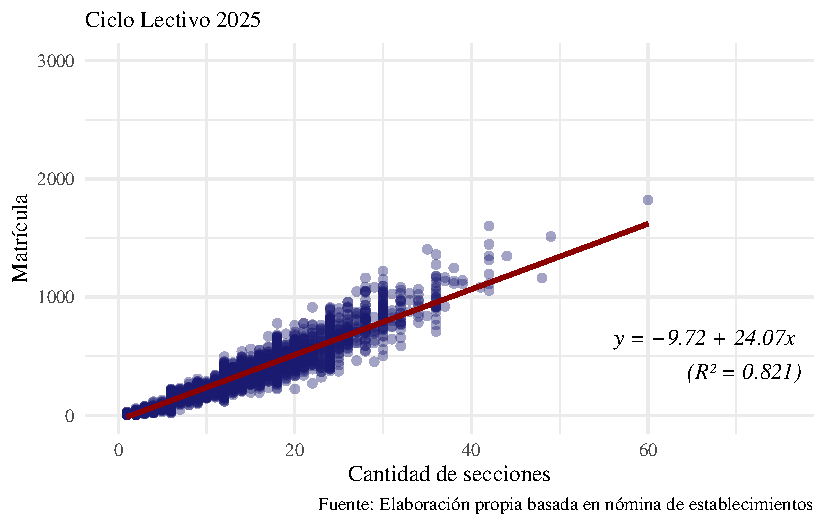
\includegraphics[keepaspectratio]{muestra_2025_files/figure-pdf/fig-matricula_seccion-1.pdf}}

}

\end{figure}%

Sin embargo, hacer un ``censo'' para las secciones pequeñas hace que se
aumente la chance de seleccionar estudiantes de secciones pequeñas que,
en general, pertenecen a establecimientos con una menor matrícula. A
continuación se muestra en la Tabla~\ref{tbl-matricula_size_seccion}
como las secciones de hasta 10 estudiantes suelen pertenecen a
establecimientos con una media y una mediana de la matrícula muy por
debajo de la que poseen las secciones más grandes.

\begin{table}

\caption{\label{tbl-matricula_size_seccion}Comparación de la media y
mediana de los establecimientos en función del tamaño de la sección (+-
10 estudiantes)}

\centering{

\fontsize{12.0pt}{14.4pt}\selectfont
\begin{tabular*}{\linewidth}{@{\extracolsep{\fill}}lcc}
\toprule
\textbf{Variable de Matrícula} & \textbf{Chicas}  N = 7.026\textsuperscript{\textit{1}} & \textbf{No chica}  N = 65.866\textsuperscript{\textit{1}} \\ 
\midrule\addlinespace[2.5pt]
{\bfseries Matrícula Inicial 2025} & 61,9 
16,0 & 461,6 
430,0 \\ 
    Desconocido & 4 & 0 \\ 
\bottomrule
\end{tabular*}
\begin{minipage}{\linewidth}
\textsuperscript{\textit{1}}Media
Mediana\\
\end{minipage}

}

\end{table}%

En cualquier caso, las reglas identificadas de la selección de los
estudiantes parece tener efectos contrapuestos y es algo difícil de
estimar el impacto de cada uno por separado. En particular es difícil de
construir ponderadores que anticipen (\emph{ex-ante}) el sesgo de estas
decisiones. Claro que siempre se podrá recurrir al recurso de los
calibradores (\emph{ex-post}) para usarlos al momento del análisis,
aunque parece una estrategia algo arriesgada.

Una opción que se puede tener cuenta en estos casos es la inclusión del
tamaño de la matrícula en la probabilidad de seleccionar al
establecimiento en la primera etapa. Esta estrategia puede tener más de
un beneficio. Uno de ellos es que permite una regla simple para la
segunda etapa. En efecto, se podría registrar una misma cantidad de
estudiantes por establecimiento de forma independiente a la cantidad de
secciones. Esto tiene el beneficio adicional que, siguiendo ese diseño,
la muestra se vuelve autoponderada lo que facilita los análisis
posteriores. Claro está que serán necesario la construcción de
calibradores que corrijan la no-respuesta, pero esto es un escenario
cualitativamente diferente al descripto en el párrafo anterior. En este
contexto, si la muestra no tiene, \emph{a posteriori}, problemas de
no-respuesta, no sería necesario la construcción de calibradores. Sin
entrar en detalles (porque en parte se entremezclan un lenguaje de
intenciones u objetivos con un lenguaje de métodos) se podría decir que
se podrían aprovechar algunas de las características que ofrece el
método conocido como muestreo proporcional al tamaño
(Sección~\ref{sec-pps}).

Por último algunos comentarios van en línea sobre el espectro de
inferencias posibles con la muestra 2023. En la biblografía sobre
muestreo se suele hacer una distinción clásica entre los
\textbf{estratos} y los \textbf{dominios} de estimación
(Sección~\ref{sec-estratificado}). Los primeros se suelen usar en el
diseño (\emph{ex-ante}) con la presunción de que en la población existen
``clases'' discretas que son parecidas en su interior y diferentes entre
sí. Si esto es así, su inclusión en el diseño trae mejoras en la
precisión en la estimación. En cambio, los dominios tienen que ver con
los objetivos o intenciones posteriores del investigador para con la
muestra. Por ejemplo, aun el contexto en que se tenga la hipótesis que
los establecimientos y los estudiantes rurales poseen fuertes
particularidades en contrapoisición a los urbanos. Un escenario es la
inclusión de ``ambito'' como variable para la estratificación y otro
escenario es que se quieran realizar inferencias para cada ámbito. En
este último caso se dice que los diferentes ámbitos son dominios de
estimación de la muestra.

Cuando los estratos con los cuales se diseñan las muestras tienen una
cantidad de casos similares la distinción con los dominios se vuelve
algo ociosa. En cambio, cuando los estratos tienen diferentes números de
casos (p.e. Urbano vs.~Rural Agrupado) y luego se desea realizar
estimaciones para todos los estratos, es importante la utilidad de la
distinción. La razón es que un muestreo estratificado proporcional
ayudará poco para tener buenas estimaciones de los dominos pequeños
(p.e. Rural Agrupado). En esos casos puede ser preferible un muestreo
estratificado con asignación no proporcional óptima (Neyman 1934).

\subsection{Evaluación actual de la muestra usada en
2024}\label{evaluaciuxf3n-actual-de-la-muestra-usada-en-2024}

Desde el momento en que se diseñó la muestra (2023), la población de
estudiantes y establecimientos fue cambiando. En especial, es notorio el
aumento de establecimientos con jornada completa en los últimos años.
Estos cambios poblacionales pueden sugerir dudas acerca de la adecuación
de una muestra que fue diseñada para representar a una población con
otras características. A pesar de estos supuestos razonables, la muestra
actual no parece ---al menos en lo que respecta a los
establecimientos--- haber quedado desfasada para captar el incremento de
la jornada completa. Más en particular, se observa una pequeña
sobrerepresentación de los establecimientos con jornada completa en esta
primera etapa de la muestra. Esto puede deberse a que la expansión de la
jornada completa se dío principalmente en establecimientos con matrícula
no muy grandes que es justamente el tipo de establecimeintos en donde la
muestra anterior parecía tener más casos. A continuación, en la
Tabla~\ref{tbl-poblacion_muestra_2024}, se comparan parámetros
poblacionales de los establecimientos con las respectivas estimaciones
de la muestra.

\begin{table}

\caption{\label{tbl-poblacion_muestra_2024}Comparación parámetros
poblacionales de establecimientos vs muestra 2024}

\centering{

\fontsize{12.0pt}{14.4pt}\selectfont
\begin{tabular*}{\linewidth}{@{\extracolsep{\fill}}lcc}
\toprule
 & \textbf{Población Total (N = 5884)} & \textbf{Muestra 2024(n = 669)} \\ 
\cmidrule(lr){2-2} \cmidrule(lr){3-3}
\textbf{Variable} & \textbf{N = 5.884}\textsuperscript{\textit{1}} & \textbf{N = 669}\textsuperscript{\textit{1}} \\ 
\midrule\addlinespace[2.5pt]
jornada\_completa &  &  \\ 
    NO & 4.757 (81\%) & 493 (74\%) \\ 
    SI & 1.127 (19\%) & 176 (26\%) \\ 
sector &  &  \\ 
    Estatal & 4.189 (71\%) & 487 (73\%) \\ 
    Privado & 1.695 (29\%) & 182 (27\%) \\ 
ambito &  &  \\ 
    Rural Agrupado & 372 (6,3\%) & 77 (12\%) \\ 
    Rural Disperso & 1.064 (18\%) & 133 (20\%) \\ 
    Urbano & 4.448 (76\%) & 459 (69\%) \\ 
matricula\_inicial\_2025 & 256 (82 – 429) & 234 (75 – 413) \\ 
    Desconocido & 10 &  \\ 
latitud & -34,77 (-35,82 – -34,59) & -34,77 (-36,19 – -34,57) \\ 
longitud & -58,69 (-59,78 – -58,40) & -58,74 (-59,98 – -58,43) \\ 
Region &  &  \\ 
    01 & 307 (5,2\%) & 29 (4,3\%) \\ 
    02 & 385 (6,5\%) & 39 (5,8\%) \\ 
    03 & 335 (5,7\%) & 35 (5,2\%) \\ 
    04 & 335 (5,7\%) & 30 (4,5\%) \\ 
    05 & 304 (5,2\%) & 26 (3,9\%) \\ 
    06 & 329 (5,6\%) & 35 (5,2\%) \\ 
    07 & 231 (3,9\%) & 29 (4,3\%) \\ 
    08 & 256 (4,4\%) & 24 (3,6\%) \\ 
    09 & 373 (6,3\%) & 40 (6,0\%) \\ 
    10 & 279 (4,7\%) & 40 (6,0\%) \\ 
    11 & 300 (5,1\%) & 32 (4,8\%) \\ 
    12 & 182 (3,1\%) & 27 (4,0\%) \\ 
    13 & 148 (2,5\%) & 24 (3,6\%) \\ 
    14 & 188 (3,2\%) & 20 (3,0\%) \\ 
    15 & 184 (3,1\%) & 19 (2,8\%) \\ 
    16 & 134 (2,3\%) & 19 (2,8\%) \\ 
    17 & 146 (2,5\%) & 18 (2,7\%) \\ 
    18 & 184 (3,1\%) & 18 (2,7\%) \\ 
    19 & 214 (3,6\%) & 35 (5,2\%) \\ 
    20 & 192 (3,3\%) & 24 (3,6\%) \\ 
    21 & 128 (2,2\%) & 14 (2,1\%) \\ 
    22 & 184 (3,1\%) & 29 (4,3\%) \\ 
    23 & 167 (2,8\%) & 20 (3,0\%) \\ 
    24 & 207 (3,5\%) & 21 (3,1\%) \\ 
    25 & 187 (3,2\%) & 21 (3,1\%) \\ 
    Desconocido & 5 & 1 \\ 
nombreDistrito &  &  \\ 
    25 de Mayo & 47 (0,8\%) & 5 (0,7\%) \\ 
    9 de Julio & 36 (0,6\%) & 6 (0,9\%) \\ 
    Adolfo Alsina & 23 (0,4\%) & 3 (0,4\%) \\ 
    Adolfo Gonzales Chaves & 15 (0,3\%) & 2 (0,3\%) \\ 
    Alberti & 12 (0,2\%) & 1 (0,1\%) \\ 
    Almirante Brown & 137 (2,3\%) & 10 (1,5\%) \\ 
    Arrecifes & 20 (0,3\%) & 5 (0,7\%) \\ 
    Avellaneda & 91 (1,5\%) & 4 (0,6\%) \\ 
    Ayacucho & 36 (0,6\%) & 4 (0,6\%) \\ 
    Azul & 54 (0,9\%) & 4 (0,6\%) \\ 
    Bahía Blanca & 95 (1,6\%) & 9 (1,3\%) \\ 
    Balcarce & 38 (0,6\%) & 3 (0,4\%) \\ 
    Baradero & 27 (0,5\%) & 5 (0,7\%) \\ 
    Benito Juárez & 13 (0,2\%) & 2 (0,3\%) \\ 
    Berazategui & 93 (1,6\%) & 8 (1,2\%) \\ 
    Berisso & 28 (0,5\%) & 2 (0,3\%) \\ 
    Bolívar & 37 (0,6\%) & 5 (0,7\%) \\ 
    Bragado & 22 (0,4\%) & 1 (0,1\%) \\ 
    Brandsen & 22 (0,4\%) & 5 (0,7\%) \\ 
    Campana & 43 (0,7\%) & 4 (0,6\%) \\ 
    Cañuelas & 39 (0,7\%) & 6 (0,9\%) \\ 
    Capitán Sarmiento & 12 (0,2\%) & 1 (0,1\%) \\ 
    Carlos Casares & 23 (0,4\%) & 1 (0,1\%) \\ 
    Carlos Tejedor & 19 (0,3\%) & 2 (0,3\%) \\ 
    Carmen de Areco & 19 (0,3\%) & 2 (0,3\%) \\ 
    Castelli & 18 (0,3\%) &  \\ 
    Chacabuco & 37 (0,6\%) & 4 (0,6\%) \\ 
    Chascomús & 37 (0,6\%) & 7 (1,0\%) \\ 
    Chivilcoy & 48 (0,8\%) & 3 (0,4\%) \\ 
    Colón & 15 (0,3\%) & 4 (0,6\%) \\ 
    Coronel de Marina L. Rosales & 26 (0,4\%) & 4 (0,6\%) \\ 
    Coronel Dorrego & 20 (0,3\%) & 1 (0,1\%) \\ 
    Coronel Pringles & 24 (0,4\%) &  \\ 
    Coronel Suárez & 35 (0,6\%) & 2 (0,3\%) \\ 
    Daireaux & 21 (0,4\%) & 2 (0,3\%) \\ 
    Dolores & 21 (0,4\%) & 2 (0,3\%) \\ 
    Ensenada & 18 (0,3\%) & 1 (0,1\%) \\ 
    Escobar & 79 (1,3\%) & 6 (0,9\%) \\ 
    Esteban Echeverría & 71 (1,2\%) & 8 (1,2\%) \\ 
    Exaltación de la Cruz & 21 (0,4\%) & 4 (0,6\%) \\ 
    Ezeiza & 46 (0,8\%) & 6 (0,9\%) \\ 
    Florencio Varela & 98 (1,7\%) & 6 (0,9\%) \\ 
    Florentino Ameghino & 9 (0,2\%) & 4 (0,6\%) \\ 
    General Alvarado & 21 (0,4\%) & 4 (0,6\%) \\ 
    General Alvear & 25 (0,4\%) &  \\ 
    General Arenales & 10 (0,2\%) & 1 (0,1\%) \\ 
    General Belgrano & 16 (0,3\%) & 2 (0,3\%) \\ 
    General Guido & 14 (0,2\%) & 1 (0,1\%) \\ 
    General Juan Madariaga & 23 (0,4\%) & 2 (0,3\%) \\ 
    General La Madrid & 16 (0,3\%) & 3 (0,4\%) \\ 
    General Las Heras & 16 (0,3\%) & 2 (0,3\%) \\ 
    General Lavalle & 8 (0,1\%) & 2 (0,3\%) \\ 
    General Paz & 25 (0,4\%) & 2 (0,3\%) \\ 
    General Pinto & 13 (0,2\%) &  \\ 
    General Pueyrredón & 167 (2,8\%) & 29 (4,3\%) \\ 
    General Rodríguez & 34 (0,6\%) & 5 (0,7\%) \\ 
    General San Martín & 98 (1,7\%) & 13 (1,9\%) \\ 
    General Viamonte & 18 (0,3\%) & 1 (0,1\%) \\ 
    General Villegas & 30 (0,5\%) & 4 (0,6\%) \\ 
    Guaminí & 18 (0,3\%) & 2 (0,3\%) \\ 
    Hipólito Yrigoyen & 9 (0,2\%) & 1 (0,1\%) \\ 
    Hurlingham & 46 (0,8\%) & 4 (0,6\%) \\ 
    Ituzaingó & 45 (0,8\%) & 5 (0,7\%) \\ 
    José C. Paz & 63 (1,1\%) & 7 (1,0\%) \\ 
    Junín & 45 (0,8\%) & 8 (1,2\%) \\ 
    La Costa & 25 (0,4\%) & 1 (0,1\%) \\ 
    La Matanza & 335 (5,7\%) & 35 (5,2\%) \\ 
    La Plata & 201 (3,4\%) & 18 (2,7\%) \\ 
    Lanús & 115 (2,0\%) & 13 (1,9\%) \\ 
    Laprida & 15 (0,3\%) & 4 (0,6\%) \\ 
    Las Flores & 39 (0,7\%) & 3 (0,4\%) \\ 
    Leandro N. Alem & 15 (0,3\%) &  \\ 
    Lezama & 12 (0,2\%) & 1 (0,1\%) \\ 
    Lincoln & 41 (0,7\%) & 2 (0,3\%) \\ 
    Lobería & 32 (0,5\%) & 4 (0,6\%) \\ 
    Lobos & 35 (0,6\%) & 5 (0,7\%) \\ 
    Lomas de Zamora & 179 (3,0\%) & 22 (3,3\%) \\ 
    Luján & 49 (0,8\%) & 7 (1,0\%) \\ 
    Magdalena & 23 (0,4\%) & 3 (0,4\%) \\ 
    Maipú & 12 (0,2\%) & 2 (0,3\%) \\ 
    Malvinas Argentinas & 81 (1,4\%) & 9 (1,3\%) \\ 
    Mar Chiquita & 26 (0,4\%) & 2 (0,3\%) \\ 
    Marcos Paz & 24 (0,4\%) & 4 (0,6\%) \\ 
    Mercedes & 44 (0,7\%) & 5 (0,7\%) \\ 
    Merlo & 120 (2,0\%) & 11 (1,6\%) \\ 
    Monte & 18 (0,3\%) & 3 (0,4\%) \\ 
    Monte Hermoso & 3 (<0,1\%) & 1 (0,1\%) \\ 
    Moreno & 138 (2,3\%) & 13 (1,9\%) \\ 
    Morón & 91 (1,5\%) & 8 (1,2\%) \\ 
    Navarro & 30 (0,5\%) & 4 (0,6\%) \\ 
    Necochea & 50 (0,9\%) & 8 (1,2\%) \\ 
    Olavarría & 74 (1,3\%) & 10 (1,5\%) \\ 
    Patagones & 28 (0,5\%) & 9 (1,3\%) \\ 
    Pehuajó & 34 (0,6\%) & 6 (0,9\%) \\ 
    Pellegrini & 6 (0,1\%) & 1 (0,1\%) \\ 
    Pergamino & 56 (1,0\%) & 8 (1,2\%) \\ 
    Pila & 15 (0,3\%) & 1 (0,1\%) \\ 
    Pilar & 112 (1,9\%) & 10 (1,5\%) \\ 
    Pinamar & 10 (0,2\%) &  \\ 
    Presidente Perón & 19 (0,3\%) & 2 (0,3\%) \\ 
    Puan & 18 (0,3\%) & 3 (0,4\%) \\ 
    Punta Indio & 15 (0,3\%) &  \\ 
    Quilmes & 144 (2,4\%) & 16 (2,4\%) \\ 
    Ramallo & 24 (0,4\%) & 3 (0,4\%) \\ 
    Rauch & 23 (0,4\%) & 2 (0,3\%) \\ 
    Rivadavia & 20 (0,3\%) & 3 (0,4\%) \\ 
    Rojas & 20 (0,3\%) &  \\ 
    Roque Pérez & 25 (0,4\%) & 5 (0,7\%) \\ 
    Saavedra & 18 (0,3\%) & 1 (0,1\%) \\ 
    Saladillo & 36 (0,6\%) & 3 (0,4\%) \\ 
    Salliqueló & 5 (<0,1\%) & 1 (0,1\%) \\ 
    Salto & 20 (0,3\%) & 3 (0,4\%) \\ 
    San Andrés de Giles & 29 (0,5\%) & 6 (0,9\%) \\ 
    San Antonio de Areco & 18 (0,3\%) & 7 (1,0\%) \\ 
    San Cayetano & 10 (0,2\%) & 1 (0,1\%) \\ 
    San Fernando & 55 (0,9\%) & 4 (0,6\%) \\ 
    San Isidro & 89 (1,5\%) & 10 (1,5\%) \\ 
    San Miguel & 91 (1,5\%) & 11 (1,6\%) \\ 
    San Nicolás & 57 (1,0\%) & 9 (1,3\%) \\ 
    San Pedro & 42 (0,7\%) & 4 (0,6\%) \\ 
    San Vicente & 31 (0,5\%) &  \\ 
    Suipacha & 14 (0,2\%) & 1 (0,1\%) \\ 
    Tandil & 62 (1,1\%) & 8 (1,2\%) \\ 
    Tapalqué & 22 (0,4\%) & 2 (0,3\%) \\ 
    Tigre & 111 (1,9\%) & 11 (1,6\%) \\ 
    Tordillo & 5 (<0,1\%) & 3 (0,4\%) \\ 
    Tornquist & 18 (0,3\%) & 4 (0,6\%) \\ 
    Trenque Lauquen & 47 (0,8\%) & 7 (1,0\%) \\ 
    Tres Arroyos & 41 (0,7\%) & 5 (0,7\%) \\ 
    Tres de Febrero & 87 (1,5\%) & 12 (1,8\%) \\ 
    Tres Lomas & 7 (0,1\%) & 1 (0,1\%) \\ 
    Vicente López & 74 (1,3\%) & 10 (1,5\%) \\ 
    Villa Gesell & 12 (0,2\%) & 1 (0,1\%) \\ 
    Villarino & 32 (0,5\%) & 6 (0,9\%) \\ 
    Zárate & 45 (0,8\%) & 8 (1,2\%) \\ 
    Desconocido & 5 & 1 \\ 
Nivel\_Modalidad\_Res &  &  \\ 
    2.Primaria & 5.879 (100\%) & 668 (100\%) \\ 
    Desconocido & 5 & 1 \\ 
Matrícula Inicial 2025 & 256 (82 – 430) & 235 (75 – 414) \\ 
    Desconocido & 15 & 1 \\ 
Secciones Inicial 2025 & 12 (6 – 18) & 12 (6 – 18) \\ 
    Desconocido & 15 & 1 \\ 
sin AUH & 153 (44 – 276) & 144 (44 – 261) \\ 
    Desconocido & 42 & 4 \\ 
sin cruce & 0,00 (0,00 – 1,00) & 0,00 (0,00 – 1,00) \\ 
    Desconocido & 42 & 4 \\ 
auh\_pct & 32 (13 – 50) & 32 (14 – 50) \\ 
    Desconocido & 48 & 4 \\ 
\bottomrule
\end{tabular*}
\begin{minipage}{\linewidth}
\textsuperscript{\textit{1}}n (\%); Mediana (Q1 -- Q3)\\
\end{minipage}

}

\end{table}%

\section{Muestra 2025}\label{muestra-2025}

Teniendo en mente las características destacadas de la muestra anterior,
ahora vamos a pasar a describir los objetivos de la muestra de 2025. Más
allá de la/s técnica/s incluida/s para llegar esos objetivos se espera:

\begin{itemize}
\item
  Incluir los mismos criterios (actualizados a valores de 2025) que
  anteriormente se incluyeron en la construcción de los estratos para la
  construcción de una muestra balanceada. Esto son:

  a) Sector (Estatal/Privado)

  b) Porcentaje de estudiantes con AUH

  c) Presencia de jornada completa

  d) Ámbito

  La idea de estos es que la muestra (de estudiantes y no de
  establecimientos) se acerque a los valores de tendencia central de
  esas variables.
\item
  Dado que algunas variables numéricas se encuentran disponibles como
  marco muestral para cada estabecimeinto también se va a exigir una
  convergencia con la distribución (esto es, no solo con sus valores de
  tendencia central) de las siguientes variables:

  a) Latitud

  b) Longitud

  c) Porcentaje de AUH

  Además, se espera complementar lo anterior con las siguientes
  probabilidades de inclusión:
\item
  Otorgarle una mayor probabilidad de entrar a la primera etapa a los
  establecimientos que entraron en la muestra anterior. La idea es hacer
  un diseño compatible con una muestra tipo panel que se renueve
  (aproximadamente) por cuartos en cada edición. De esta manera, ningun
  establecimiento estaría más de 4 años seguidos y, de manera
  complementaria, el cuarto que se renueva permitiría ajustar la muestra
  a los cambios poblacionales sucedidos en el último año.
\item
  Otorgarle una probabilidad de entrar en la primera etapa a los
  establecimientos en función del tamaño de la matrícula.
\end{itemize}

\noindent Esto último quizá merezca algo más de justificación porque
puede parecer contraintuitivo. En efecto, que en la primera etapa los
establecimientos sean seleccionados en función del tamaño de la
matrícula permite que, para la segunda etapa de la muestra, se pueda
tener una regla simple como la asignación de un número fijo de
estudiantes para cada establecimiento. Esto, además, permite (en
ausencia de problemas de no-respuesta) hacer análisis con una muestra
autoponderada. Más concretamente se aspira a registrar 10 estudiantes de
cada establecimiento.

En los establecimientos en donde haya más de una sección, se puede
sortear entre las secciones disponibles y quedarse, en principio, con
una de ellas. Previamente se puede generar un número para cada
caso/establecimiento seleccionado que ordene a los establecimientos en
función de algún criterio (p.e. matrícula). Algunos establecimientos
tendran un número par y otros tendrán uno impar. En este sentido, una
vez sorteada la sección, se usa el valor del número anterior para
indicar el modo de selección de los 10 estudaintes. Si ese
establecimiento posee un número par, se elige a los primeros 10
estudiantes. Si ese establecimeinto posee un número impar, se elige los
últimos 10 estudiantes. Si la sección seleccionada se agota sin llegar a
los 10 casos se pasa a una sección siguiente siguiendo el mismo criterio
de selección de los estudiantes que en la sección anterior.

De este modo se tiene una regla no arbitraria (en el sentido que no
decide el docente o el establecimiento qué caso cargar), la misma parece
ser probabilística y, de manera derivada, permite trabajar (en ausencia
de problemas de no-respuesta) con los datos sin ponderar.

\begin{verbatim}
[1] 676
\end{verbatim}

\begin{verbatim}
[1] 675
\end{verbatim}

\section{Resultados muestra 2025}\label{resultados-muestra-2025}

Teniendo presente las restricciones anteriores se realizó una muestra
con los siguientes resultados a nivel de establecimientos. Se recuerda
que la muestra aspira a ser una muestra de estudiantes más que de
establecimientos por lo que algunas desviaciones en esta etapa son más
esperables que otras. En particular, es esperable que la media de la
matrícula de los establecimientos seleccionados sea mayor a la media de
la matrícula de la población de establecimientos. Algunos de los
resultados, principalmente en cuanto a valores de tendencia central, se
pueden ver en la Tabla~\ref{tbl-poblacion_muestra_2025}.

\begin{table}

\caption{\label{tbl-poblacion_muestra_2025}Comparación parámetros
poblacionales de establecimientos vs muestra 2025}

\centering{

\fontsize{12.0pt}{14.4pt}\selectfont
\begin{tabular*}{\linewidth}{@{\extracolsep{\fill}}lcc}
\toprule
 & \textbf{Población Total (N = 5836)} & \textbf{Muestra 2025(n = 675)} \\ 
\cmidrule(lr){2-2} \cmidrule(lr){3-3}
\textbf{Variable} & \textbf{N = 5.836}\textsuperscript{\textit{1}} & \textbf{N = 675}\textsuperscript{\textit{1}} \\ 
\midrule\addlinespace[2.5pt]
sector &  &  \\ 
    Estatal & 4.157 (71\%) & 438 (65\%) \\ 
    Privado & 1.679 (29\%) & 237 (35\%) \\ 
ambito &  &  \\ 
    Rural Agrupado & 371 (6,4\%) & 23 (3,4\%) \\ 
    Rural Disperso & 1.039 (18\%) & 20 (3,0\%) \\ 
    Urbano & 4.426 (76\%) & 632 (94\%) \\ 
matricula\_inicial\_2025 & 257 (85 – 430) & 390 (268 – 553) \\ 
latitud & -34,77 (-35,81 – -34,59) & -34,72 (-34,92 – -34,56) \\ 
longitud & -58,69 (-59,78 – -58,40) & -58,61 (-58,82 – -58,38) \\ 
auh\_pct & 32 (13 – 50) & 37 (16 – 53) \\ 
muestra\_2024 &  &  \\ 
    SI & 665 (100\%) & 433 (100\%) \\ 
    Desconocido & 5.171 & 242 \\ 
\bottomrule
\end{tabular*}
\begin{minipage}{\linewidth}
\textsuperscript{\textit{1}}n (\%); Mediana (Q1 -- Q3)\\
\end{minipage}

}

\end{table}%

\section{Chequeos de distribución a nivel de
establecimientos}\label{chequeos-de-distribuciuxf3n-a-nivel-de-establecimientos}

Dado que la muestra no es solo balanceada en sus medidas de tendencia
central, sino también en la distribución de otras covariables ahora
veremos justamente como la distribución de la muestra difiere, en las
variables latitud, longitud (\textbf{?@fig-mapa\_muestra\_2025}) y
porcentaje de AUH (Figura~\ref{fig-densidad_auh}), de la distribución de
las mismas a nivel del marco muestral.

\begin{figure}

\caption{\label{fig-mapa_calor_poblacion_muestra}Mapa de calor sobre la
distribución de los casos. Población y muestra 2025.}

\centering{

\pandocbounded{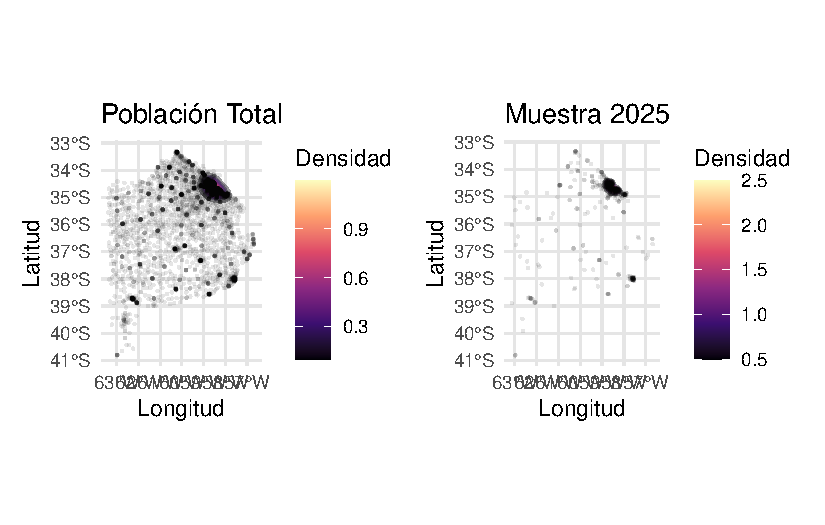
\includegraphics[keepaspectratio]{muestra_2025_files/figure-pdf/fig-mapa_calor_poblacion_muestra-1.pdf}}

}

\end{figure}%

\begin{figure}

\caption{\label{fig-densidad_auh}}

\centering{

\pandocbounded{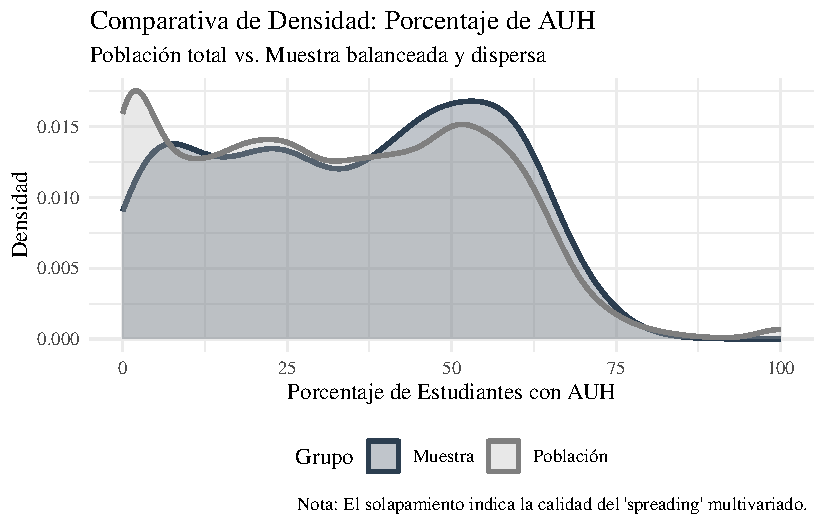
\includegraphics[keepaspectratio]{muestra_2025_files/figure-pdf/fig-densidad_auh-1.pdf}}

}

\end{figure}%

\section{Simulación a nivel de
estudiantes}\label{simulaciuxf3n-a-nivel-de-estudiantes}

Dado que en el actual diseño se emplea una muestra en donde la
probabilidad de inclusión deviene en parte del tamaño del
establecimiento es esperable, como se anticipó más arriba, encontrar
diferencias entre las tendencias centrales de algunas variables
consideradas importantes entre la muestra de establecimientos y la
población de los mismos. Por esta razón, partiendo del marco muestral de
los establecimientos vamos a crear una población sintética de
estudiantes en función de la matrícula de cada uno de ellos. Luego vamos
a comparar esa población con otra población de estudiantes asumiendo que
se seleccionan ``x'' (10 en este caso) estudiantes por cada
establecimiento seleccionado.

\begin{table}

\caption{\label{tbl-poblacion_estudiantes_vs_muestra_estudiantes}Comparación
entre poblaciónes sintéticas de estudiantes}

\centering{

\fontsize{12.0pt}{14.4pt}\selectfont
\begin{tabular*}{\linewidth}{@{\extracolsep{\fill}}lcc}
\toprule
\textbf{Variable} & \textbf{Muestra de Estudiantes (k=10)}  N = 6.750\textsuperscript{\textit{1}} & \textbf{Población de Estudiantes}  N = 1.666.253\textsuperscript{\textit{1}} \\ 
\midrule\addlinespace[2.5pt]
sector &  &  \\ 
    Estatal & 4.380 (65\%) & 1.081.271 (65\%) \\ 
    Privado & 2.370 (35\%) & 584.982 (35\%) \\ 
ambito &  &  \\ 
    Rural Agrupado & 230 (3,4\%) & 22.877 (1,4\%) \\ 
    Rural Disperso & 200 (3,0\%) & 21.001 (1,3\%) \\ 
    Urbano & 6.320 (94\%) & 1.622.375 (97\%) \\ 
matricula\_inicial\_2025 & 390 (268 – 553) & 452 (313 – 624) \\ 
jornada\_completa &  &  \\ 
    NO & 5.720 (85\%) & 1.485.455 (89\%) \\ 
    SI & 1.030 (15\%) & 180.798 (11\%) \\ 
latitud & -34,72 (-34,92 – -34,56) & -34,72 (-34,88 – -34,57) \\ 
longitud & -58,61 (-58,82 – -58,38) & -58,59 (-58,79 – -58,36) \\ 
auh\_pct & 37 (16 – 53) & 38 (18 – 54) \\ 
muestra\_2024 &  &  \\ 
    SI & 4.330 (100\%) & 182.586 (100\%) \\ 
    Desconocido & 2.420 & 1.483.667 \\ 
\bottomrule
\end{tabular*}
\begin{minipage}{\linewidth}
\textsuperscript{\textit{1}}n (\%); Mediana (Q1 -- Q3)\\
\end{minipage}

}

\end{table}%

\begin{figure}

\caption{\label{fig-poblacion_estudiantes_vs_muestra_estudiantes}}

\centering{

\pandocbounded{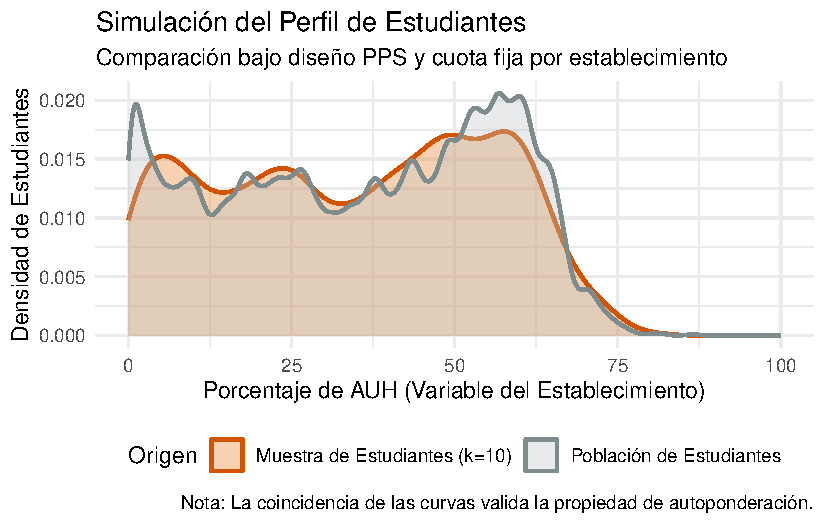
\includegraphics[keepaspectratio]{muestra_2025_files/figure-pdf/fig-poblacion_estudiantes_vs_muestra_estudiantes-1.pdf}}

}

\end{figure}%

Cabe destacar que si se realiza algún test estadístico entre ambas
distribuciones (p.e. Kolmogorov-Smirnov) se observa un aceptable ajuste
entre ambas distribuciones lo que sugiere que la muestra logra
``copiar'' aceptablemente la distribución (y no solo la tendencia
central) poblacional de la variable posesión de AUH.

\bookmarksetup{startatroot}

\chapter{Referencias
Bibliográficas}\label{referencias-bibliogruxe1ficas}

\protect\phantomsection\label{refs}
\begin{CSLReferences}{1}{1}
\bibitem[\citeproctext]{ref-baker2013}
Baker, Reg, Michael Brick, Nancy Bates, et~al. 2013. \emph{Report of the
AAPOR task force on non-probability sampling}.

\bibitem[\citeproctext]{ref-brus2022}
Brus, Dick. 2022. \emph{Spatial sampling with R}. Chapman \& Hall /CRC.

\bibitem[\citeproctext]{ref-bunge1974a}
Bunge, M. 1974. \emph{Semantics}. Dordrecht. Reidel.

\bibitem[\citeproctext]{ref-campbell1963}
Campbell, Donald, y Julian Stanley. 1963. \emph{Experimental and
quasi-experimental designs for research}. Houghton Mifflin Company.

\bibitem[\citeproctext]{ref-deville2004}
Deville, Jean, y Yves Tillé. 2004. {«Efficient balanced sampling: The
cube method»}. \emph{Biometrika} 91 (4): 893-912.

\bibitem[\citeproctext]{ref-elliott2017}
Elliott, Michael, y Richard Valliant. 2017. {«Inference for
nonprobability samples»}. \emph{Statistical Science} 32 (2): 249-64.

\bibitem[\citeproctext]{ref-everitt2011}
Everitt, Brian, Sabine Landau, Morven Leese, y Daniel Stahl. 2011.
\emph{Cluster Analysis}. 5 Edition. Wiley.

\bibitem[\citeproctext]{ref-fienberg1988}
Fienberg, Stephen, y Judith Tanur. 1988. {«From the inside out and the
outside in: Combining experimental and sampling structures»}. \emph{The
Canadian Journal of Statistics} 16 (2): 135-51.

\bibitem[\citeproctext]{ref-gigerenzer1997}
Gigerenzer, Gerd, Zeno Swijtink, Theodore Porter, John Beatty, y Lorenz
Krüger. 1997. \emph{The empire of chance}. Cambridge University Press.

\bibitem[\citeproctext]{ref-hacking2004}
Hacking, Ian. (1990) 2004. \emph{The taming of chance}. Cambridge
University Press.

\bibitem[\citeproctext]{ref-hacking2006}
Hacking, Ian. 2006. \emph{The emergence of probability: A philosophical
study of early ideas about probability, induction and statistical
inference}. Cambridge University Press.

\bibitem[\citeproctext]{ref-hedlin2015}
Hedlin, Dan. 2015. \emph{Why are design in survey sampling ad design of
randomised experiments separate areas of statistical science?}

\bibitem[\citeproctext]{ref-kish1980}
Kish, Leslie. 1980. {«Design and estimations for domains»}. \emph{The
Statistician} 29 (4): 209-22.

\bibitem[\citeproctext]{ref-kish1987}
Kish, Leslie. 1987. \emph{Statistical design for research}. John Wiley.

\bibitem[\citeproctext]{ref-klima2022}
Klima, Gyula. 2022. \emph{The medieval problem of universals}. Spring
2022. Editado por Edward Zalta. Stanford University.

\bibitem[\citeproctext]{ref-lumley2010}
Lumley, Thomas. 2010. \emph{Complex surveys. A guide to analysis using
R}. John Wiley \& Sons.

\bibitem[\citeproctext]{ref-lundstruxf6m2009}
Lundström, Sixten, y Carl Erik Särndal. 2009. \emph{Calibration of
weights in surveys with nonresponse and frame imperfections}. (Bilbao),
enero 26.

\bibitem[\citeproctext]{ref-morgan2015}
Morgan, Stephen, y Christopher Winship. 2015. \emph{Counterfactuals and
Causal Inference}. Second Edition. Cambridge University Press.

\bibitem[\citeproctext]{ref-neyman1934}
Neyman, Jerzy. 1934. {«On the Two Different Aspects of the
Representative Method: The Method of Stratified Sampling and the Method
of Purposive Selection»}. \emph{Journal of the Royal Statistical
Society} 97 (4): 558-625.

\bibitem[\citeproctext]{ref-pearl2018a}
Pearl, J. 2018. \emph{The Book of Why}. New York. Basic Books.

\bibitem[\citeproctext]{ref-platuxf3n2002}
Platón. 2002 {[}370AVC{]}. \emph{Phaedrus}. Oxford University Press.

\bibitem[\citeproctext]{ref-schneider2024}
Schneider, Ben. 2024. \emph{Simulation-based variance estimation for the
cube method}.
\url{https://www.practicalsignificance.com/posts/cube-method-simulating-joint-probs/}.

\bibitem[\citeproctext]{ref-small2019}
Small, Mario, y Laura Adler. 2019. {«The role os space in the formation
of social ties»}. \emph{Anual Review of Sociology} 45: 111-32.

\bibitem[\citeproctext]{ref-subsecretaruxeda2024}
{Subsecretaría, de planeamiento}. 2024. \emph{PRUEBAS ESCOLARES
BONAERENSES EN EL NIVEL PRIMARIO Resultados de Matemática y de Prácticas
del Lenguaje en 3°, 5° y 6°}.

\bibitem[\citeproctext]{ref-subsecretaruxeda2025}
{Subsecretaría, de planeamiento}. 2025. \emph{Qué son las pruebas
escolares bonaerenses? Evaluación formativa para la mejora de la
enseñanza y de los aprendizajes}. Subsecretaría de Planeamiento,
Dirección Provincial de Evaluación e Investigación.

\bibitem[\citeproctext]{ref-tilluxe92010}
Tillé, Yves. 2010. \emph{Balanced sampling by means of the cube method}.
(Euskal).

\bibitem[\citeproctext]{ref-tilluxe92011}
Tillé, Yves. 2011. {«Ten years of balanced sampling with the cube
method: An appraisal»}. \emph{Survey Methodology} 37 (2): 215-26.

\bibitem[\citeproctext]{ref-tilluxe92013}
Tillé, Yves, y Anton Grafström. 2013. {«Doubly balanced spatial sampling
with spreading and restitution of auxiliary totals»}.
\emph{Environmetrics} 24 (2): 120-31.

\bibitem[\citeproctext]{ref-tilluxe92023}
Tillé, Yves, y Alina Matei. 2023. \emph{Package {"}sampling{"}}.

\end{CSLReferences}




\end{document}
